% !TEX root = mythesis.tex

%==============================================================================
\chapter{Analysis}
\label{chap:multivariate_analysis}

This chapter describes the setup that will be used in the final fit to the data and the expected signal and background events described in chapter \ref{chap:data_MC}. 

Section \ref{sec:strategy} gives an overview of the fit used for extracting a cross-section measurement. Section \ref{sec:NN} presents the signal and background separation procedure, where an artificial neural network is used as multivariate classification technique.  Section \ref{sec: Profile_likehihood} gives a basic idea of binned profile likelihood fit which is used is used for signal extraction in this thesis. Section \ref{sec:systematics} explains in short about the systematic uncertainties that can modify the rate of the signal and background process. Section \ref{subsec:fittedregions} gives an overview of the fitted regions along with corresponding distributions. Finally, binning optimisation is presented in section \ref{subsec:binningoptimization}. 

%==============================================================================
\section{Cross-section measurement analysis strategy}
\label{sec:strategy}

The strategy of this analysis is to determine the signal strength $\mu_{tZq}$ (POI) of the tZq process, hence the total cross-section while including systematic uncertainties as nuisance parameter in the profile likelihood fit as described in section \ref{sec: Profile_likehihood}. Two different signal regions as defined in section \ref{sec:SR}, with different amount of signal and background contributions, are used to determine $\mu_{tZq}$. As defined in section \ref{sec:CR}, control regions are defined  to determine the normalization of the respective dominant background processes. Both the signal and three backgrounds, $t\Bar{t}$ + tW and Z+jets , \& $t\Bar{t}Z$ normalization factors are fitted as free parameters in all eight regions simultaneously. The contributions of all other backgrounds are set to their expected values and are allowed to vary within their systematic uncertainties, which are included as nuisance parameter in the fit. For the cross-section of tZq, where the Z boson decays into the charged leptons ($e^{+}e^{-}$, $\mu^{+}\mu^{-}$), $\sigma_{tl^{+}l^{-}q}$ = 102 fb is assumed to be the nominal value \cite{tZq2020} for the fit. which corresponds to the signal strength of $\mu = 1$.


\section{Multivariate analysis technique: Artificial Neural Network (NN)}
\label{sec:NN}
In order to separate the signal and background for the SM tZq processes, a cut-and-count analysis is difficult and will give bad sensitivity, due to the large number of background events and the big uncertainties associated to them. In high energy physics,  multivariate analysis techniques such artificial neural networks (NN's) have been used or proposed as good candidates for tasks of signal versus background classification.

\begin{figure}[h!] 
  \begin{subfigure}[b]{0.49\linewidth}
    \centering
    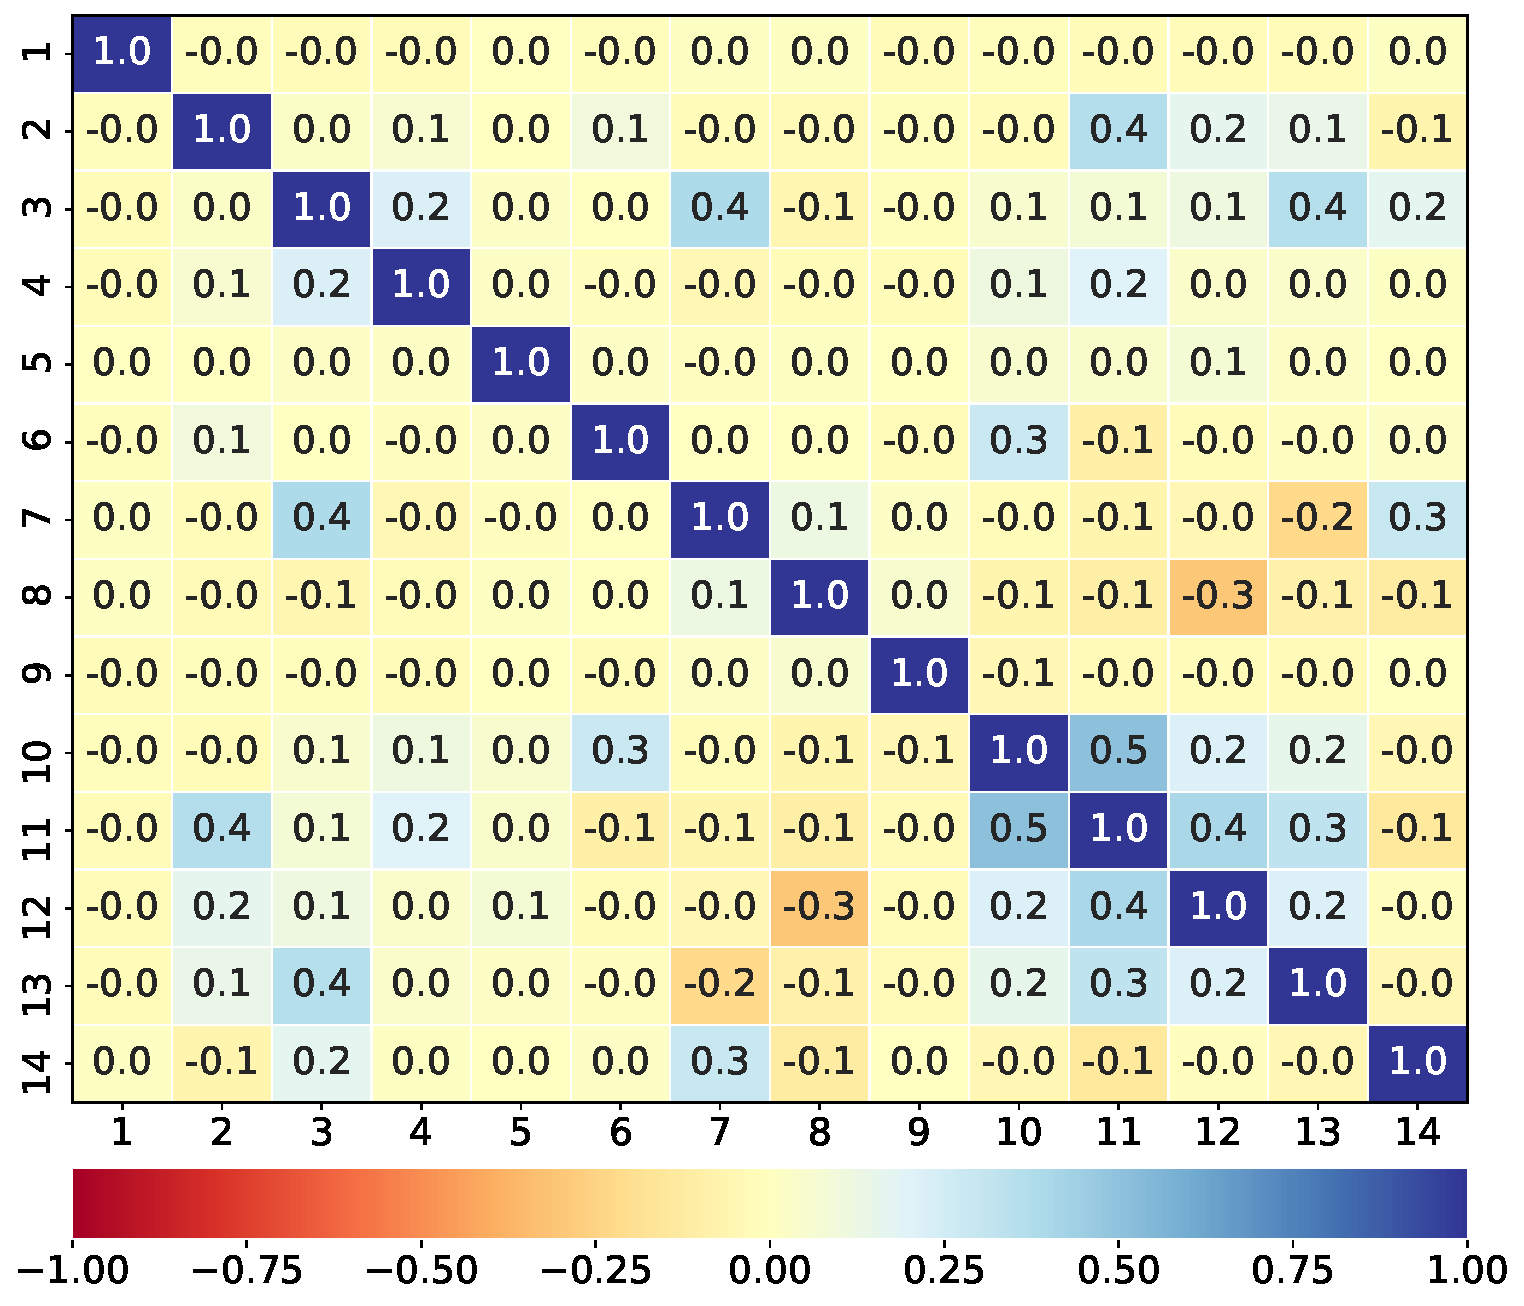
\includegraphics[width=\textwidth]{ubonn-thesis/Chapters/Chapters_06/Figure/Neural Network/SR_2j1b_correlation.pdf}
    \caption{}
    \end{subfigure}%% 
  \begin{subfigure}[b]{0.5\linewidth}
    \centering
    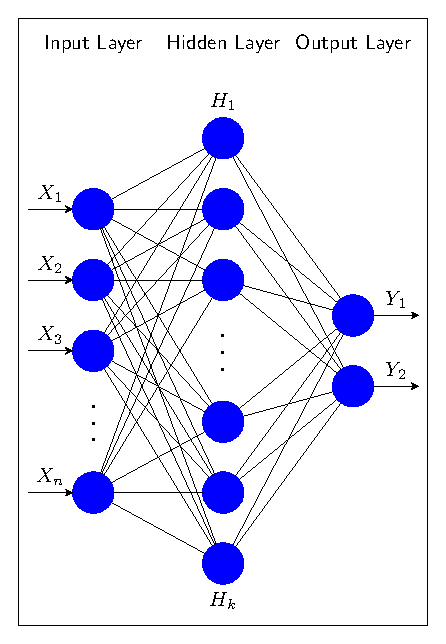
\includegraphics[width=0.6\linewidth]{ubonn-thesis/Chapters/Chapters_06/Figure/Neural Network/neural_network.pdf} 
    \caption{}
    \label{NN_config}
  \end{subfigure}
  \caption{ a) Correlation matrix between the input variables used for training in the SR 2j1b . b) Neural network configuration used for training. It is drawn using tikZ package in latex. Meaning of variables and numbers given in table \ref{tab:NN_input}}
  \label{fig:NN_configuration}
  \end{figure}


An artificial neural network (NN) is a simplified mathematical structure inspired from the real biological neural networks. It has similar basic concepts of a real biological neural network (neuron, connection strength, input linearity, output-linearity) but in a much more conservative level of complexity. The neuron is a mathematical entity which has a real value depending on the connection strengths (weights) and the values of the other neurons with which it is connected. The non-linear function that relates the output from the neuron with the weights and the inputs to the neuron is usually called \textit{activation function}. A neural network can be structured as layers. The input layer, from where the NN is fed with the input variables of the problem to be solved, followed by a number of layers called hidden layers, and finally the output layers.


An example of a multi-layer neural network is shown in figure \ref{NN_config}. Let us consider a multi-layer neural network having a layer of n input neurons $X_{i}$ (i=1,\dots,n), with an activation function $f_{X_{i}}$, a hidden layer of m neurons $H_{j}$ (j=1,\dots,m) with activation function $f_{H_{j}}$and an output layer of two neurons $Y_{p}$ (p=1,2) with activation function $f_{Y_{p}}$. The output node gives continuous output ($O_{NN}$) between 0 and 1, where the output tends to 0 for background, and +1 for signal. The neural network output is calculated as follows:

\begin{equation}
    \label{eqn:NNout}
     Y_{p} = f_{Y_{p}}(\zeta_{Y_{p}}) = f_{Y_{p}}\left( \sum_{j=1}^{m+1} w_{pj}f_{H_{j}}(\zeta_{H_{j}}) \right) = f_{Y_{p}}\left( \sum_{j=1}^{m+1} w_{pj}f_{H_{j}}\left( \sum_{i=1}^{n+1} v_{ji}f_{X_{i}}(X_{i}) \right) \right)
\end{equation}

where $w_{pj}$ are the weights between the input layer and the hidden layer, and $v_{ji}$ are the weights between the hidden layer and the output layer.

In this analysis a supervised neural network with three-layer feed-forward algorithm is implemented using Tensflow in Python \cite{tensorflow_developers_2021_5799851}.  Elu is used as activation function for both input and hidden layers whereas sigmoid for output layer. The response curve for various activation functions including elu and sigmoid can be seen in ref. \cite{nwankpa2018activation}.



\subsection{Input variables}
The input variables are chosen in an iterative process. First, many variables are used to train preliminary NN. The correlations between variables in MC events are determined. In the second step, the relevant variables with the biggest separation power are investigated by comparing the MC distributions. The signal event signature is simple as defined in section \ref{sec:SR}. Thus, the input variables are limited and can be categorized as: variables measured directly in the detector, others which are reconstructed from the measured quantities as described in section \ref{sec:event_reconstruction}. All possible variables such as momenta, relative angles, pseudo-rapidity, and particle masses are explored. The  variables used to train the NN in the SR 2j1b, SR 3j1b, CR 3j2b, and CR 4j2b are listed with their rank in table \ref{tab:NN_input}. The ranking of variables is done by comparing the statistics value obtained after training the NN with and without the variable. So, the training is repeated as many times as there are variables in list. The statistics is obtained by performing the t-test of the output of NN for the two cases. 

\begin{table}[h!]
\centering
\begin{adjustbox}{width=\textwidth}
\begin{tabular}{@{} *4l  @{}}
\toprule
Variable & \multicolumn{2}{c}{Rank} & Definition \\
 & SR 2j1b & SR 3j1b &  \\
 \midrule
 $m_{bj_{f}}$ & 1 & 1 & (Largest) invariant mass of the b-jet and the untagged jet(s) \\[0.2ex]
 $m_{t}$   &  2 &  2 & Reconstructed top-quark mass \\[0.2ex]
 $p_{T}(W)$     &  3 & 3 & $p_{T}$ of the reconstructed W boson \\[0.2ex]
 $p_{T}(Z)$    & 4 &  4 & $p_{T}$ of the reconstructed Z boson \\[0.2ex]
 $p_{T}(j_{f})$    & 5 & 5 & $p_{T}$ of the forward jet\\[0.2ex]
 $p_{T}(\ell_{W})$ & 6 & 7 & $p_{T}$ of the lepton from the W-boson decay\\[0.2ex]
 $m_{Z}$   & 7 & 8 & Mass of the reconstructed Z boson\\[0.2ex]
 $m_{T}(\ell,E_{T}^{miss})$ &  8 &  9 & Transverse mass of the W boson \\[0.2ex]
 $|\eta(\ell_{W})|$ &  9 & 10 & Absolute value of the $\eta$ of the lepton from the W boson decay\\[0.2ex]
 $|\eta(j_{f})|$  &  10 &  12 & Absolute value of the $\eta$ of the forward jet\\[0.2ex]
$\Delta R(j_{f},Z)$ & 11 &  14 &  $\Delta R$ between the forward jet and the reconstructed Z boson \\[0.2ex]
b-tagging score   &  12 & 15 & b-tagging score of the b-jet \\[0.2ex]
$|\eta(Z)|$  & 13 & 13 & Absolute value of the $\eta$ of the reconstructed Z boson \\[0.2ex]
$E_{T}^{miss}$ & 14 & 16 & Missing transverse momentum \\[0.2ex]
$p_{T}(j_{r})$  &{--}& 6  & $p_{T}$ of the radiation jet \\[0.2ex]
$|\eta(j_{r})|$     & {--} &  11 & Absolute value of the $\eta$ of the $j_{r}$ jet \\[0.2ex]
\bottomrule
\end{tabular}
\end{adjustbox}
\caption{Variables used as input to the neural network in SR 2j1b and SR 3j1b. The ranking of the variables in each of the SRs is given in the 2nd and 3rd columns, respectively.}
\label{tab:NN_input}
\end{table}  


\subsection{Data and MC comparison}

Since the neural network is trained with simulated events, it is important to check if the input variables
are modelled correctly. Data and MC distributions are compared in figures \ref{fig_signal1}, \ref{fig_signal2}, \ref{fig_signal3}, \ref{fig_signal4} and \ref{fig_signal5}. All MC distributions are normalised using their predicted cross-section values. Kolmogorov-Smirnov test (KS-test) and Chi-Square ($\chi^{2}$-test) are performed for each distributions. The p-value obtained during the test is shown along with the distributions. Technically, KS-test is used to decide if a sample comes from a population with a specific distribution. 

\begin{figure}[!h] 
  \begin{subfigure}[b]{0.33\linewidth}
    \centering
    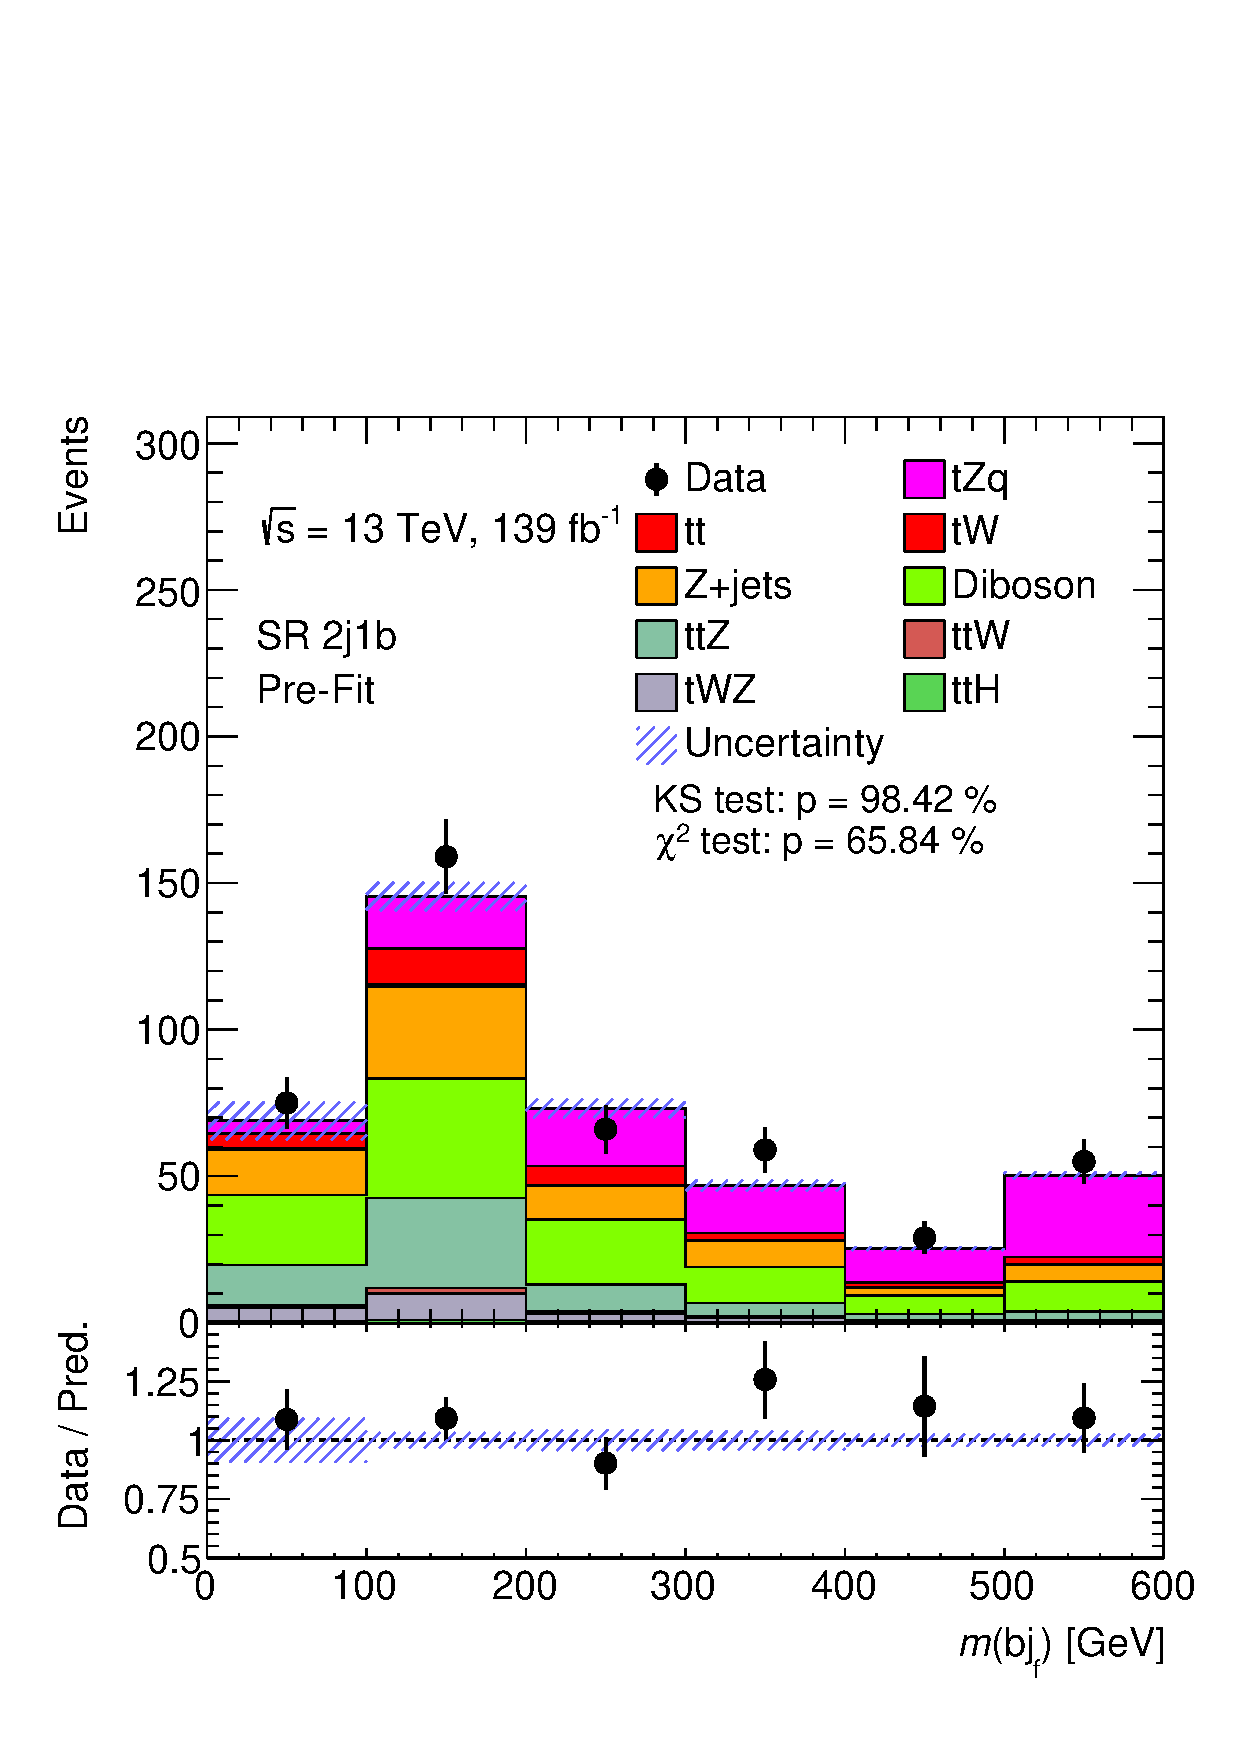
\includegraphics[width=\linewidth]{ubonn-thesis/Chapters/Chapters_06/Figure/Input_distribution/SR_2j1b_M_bj.pdf} 
  \end{subfigure}%% 
  \begin{subfigure}[b]{0.33\linewidth}
    \centering
    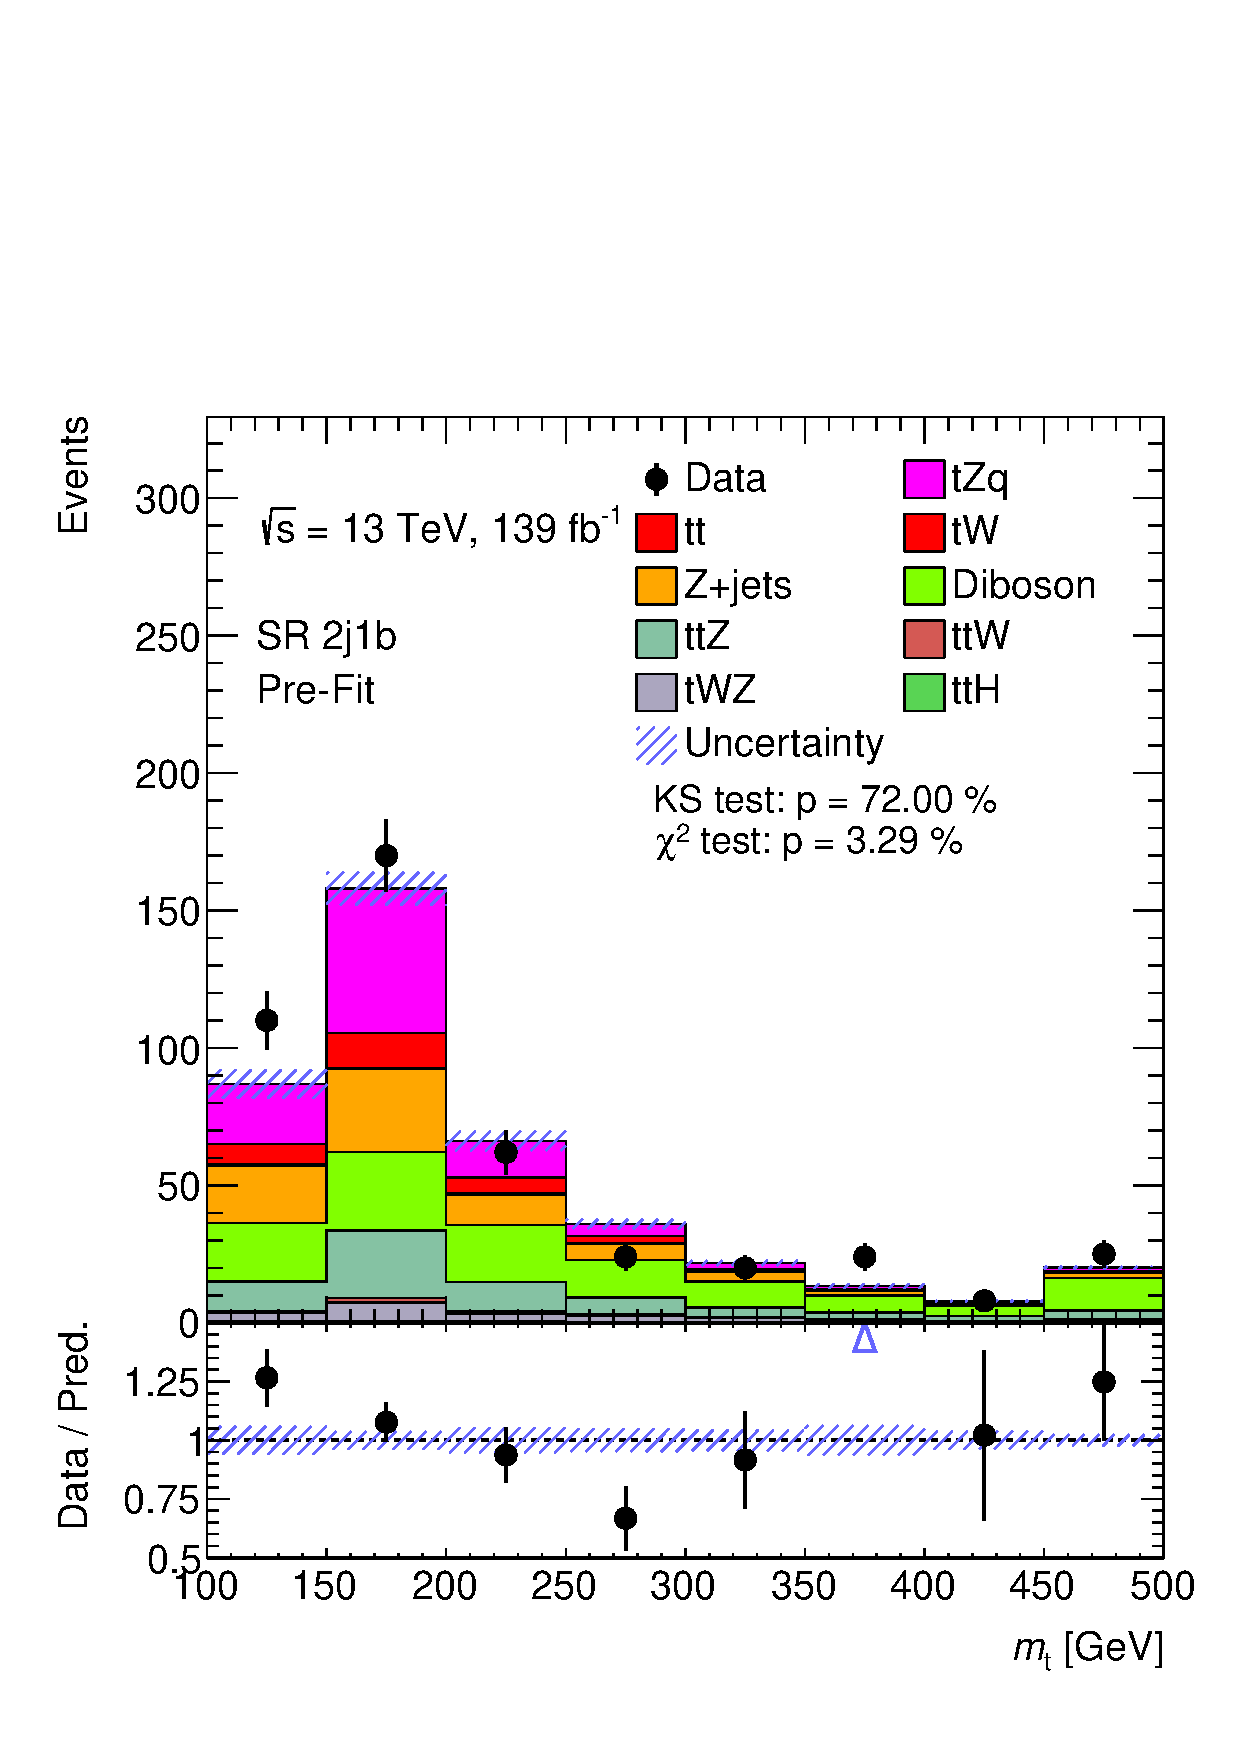
\includegraphics[width=\linewidth]{ubonn-thesis/Chapters/Chapters_06/Figure/Input_distribution/SR_2j1b_Top_mass.pdf} 
  \end{subfigure} 
  \begin{subfigure}[b]{0.33\linewidth}
    \centering
    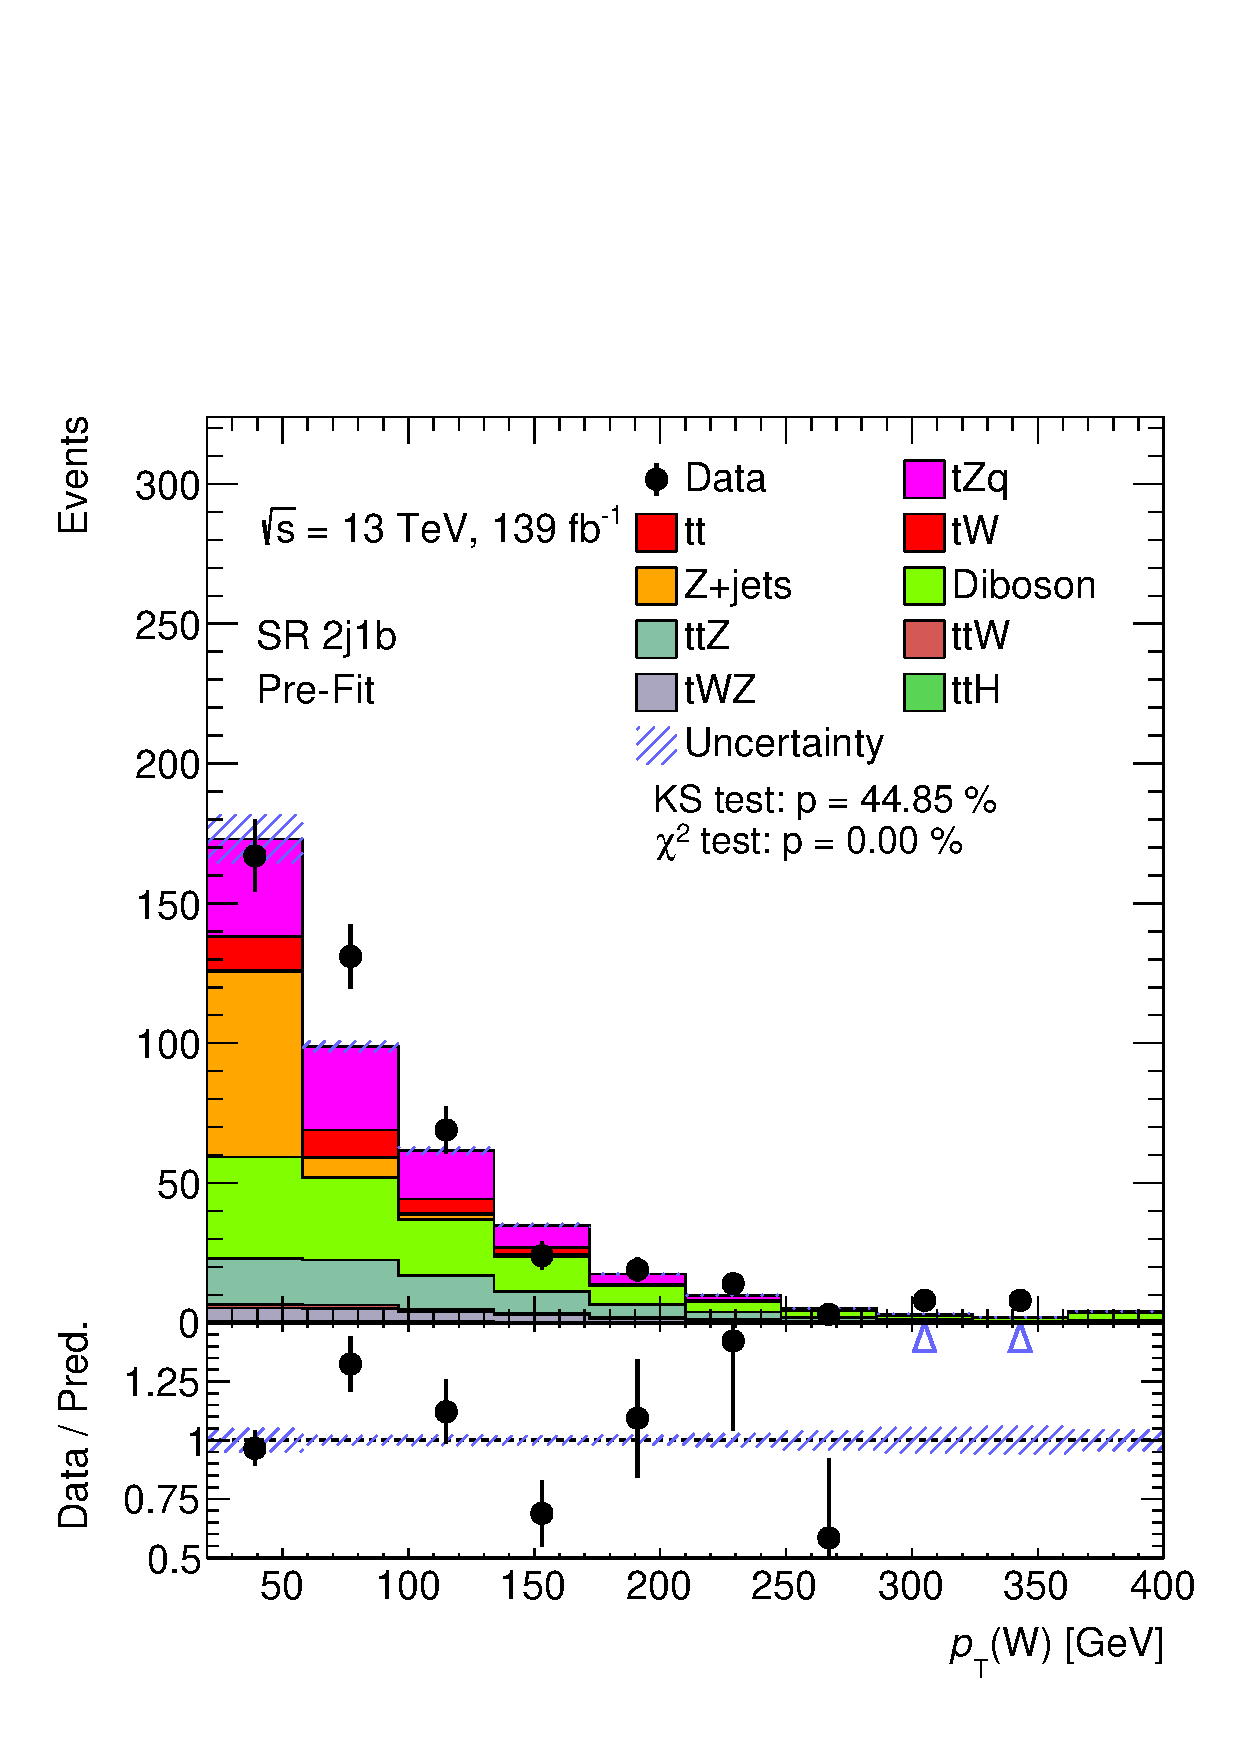
\includegraphics[width=\linewidth]{ubonn-thesis/Chapters/Chapters_06/Figure/Input_distribution/SR_2j1b_W_pt.pdf} 
  \end{subfigure}%%
  \newline
  \begin{subfigure}[b]{0.33\linewidth}
    \centering
    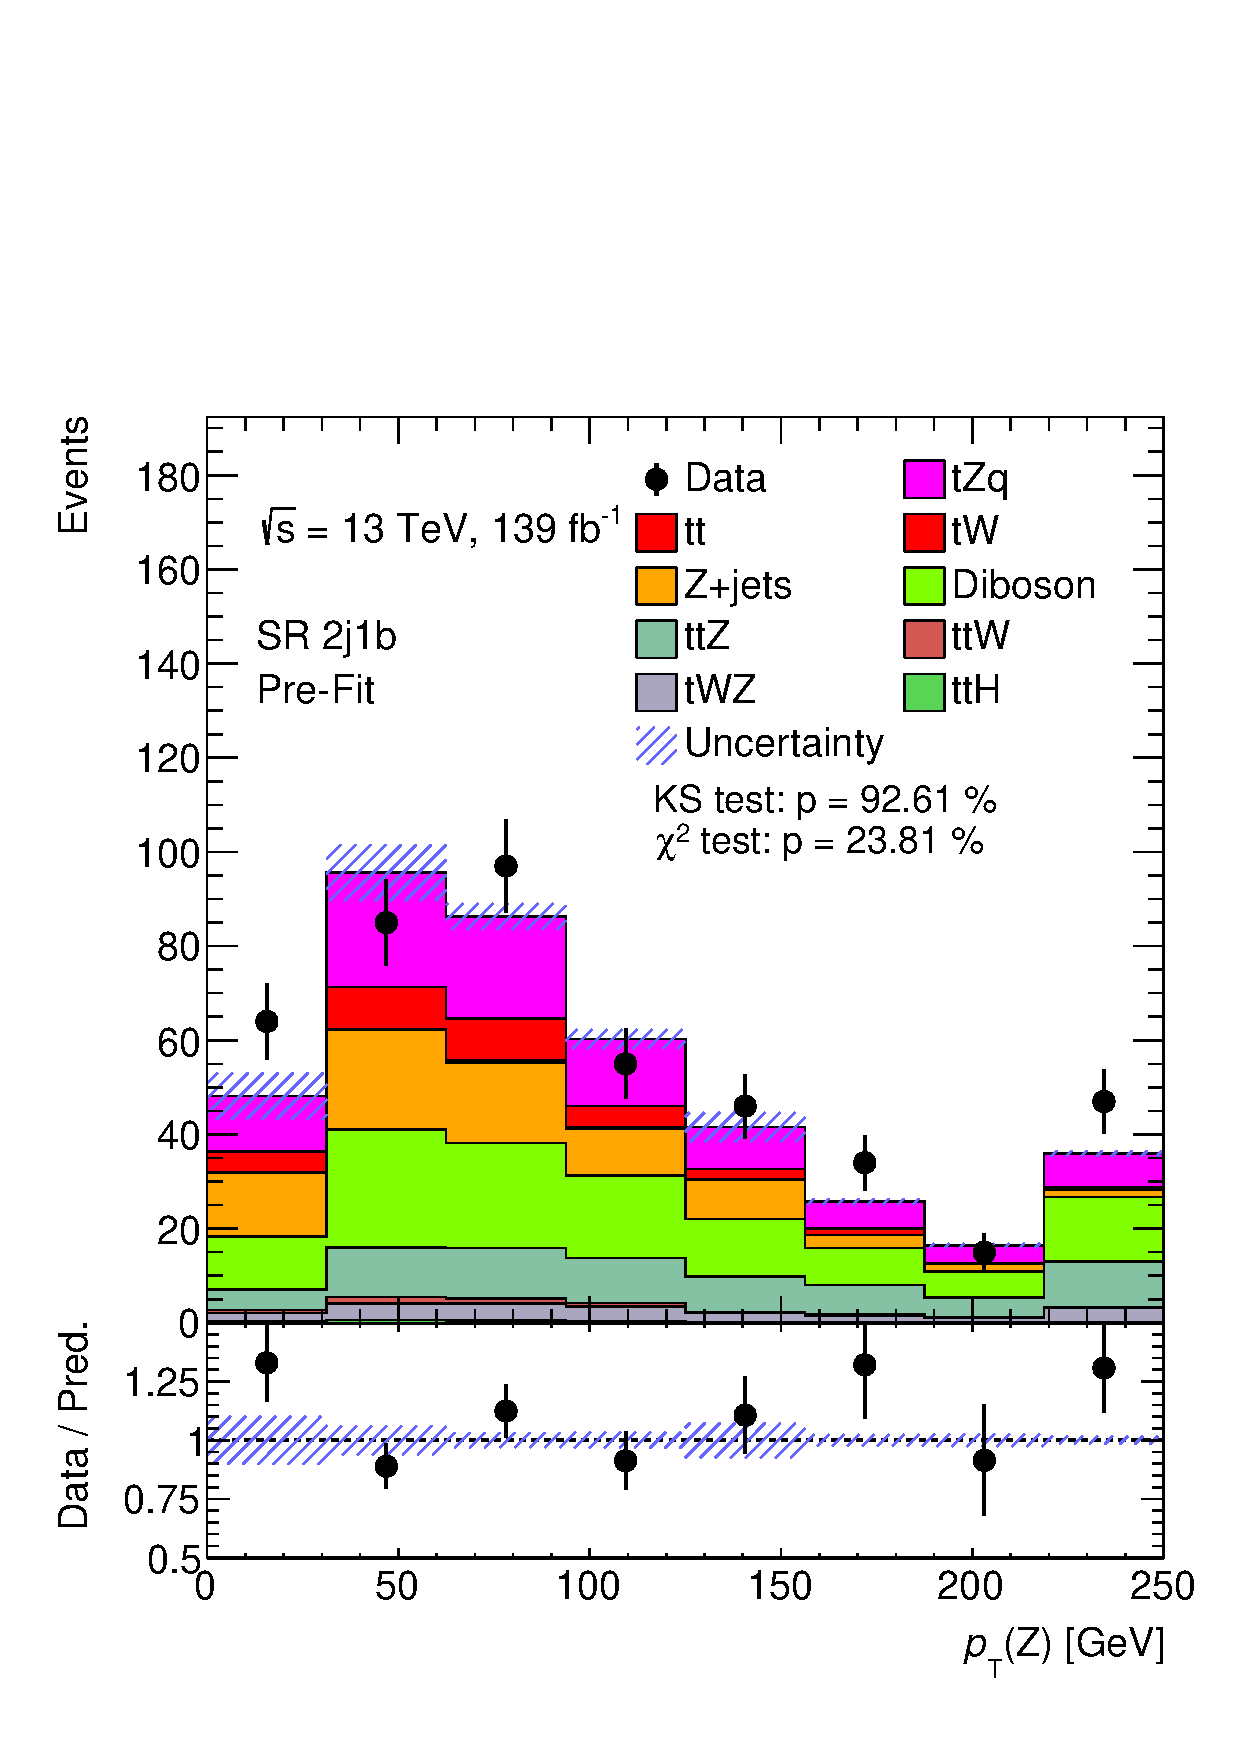
\includegraphics[width=\linewidth]{ubonn-thesis/Chapters/Chapters_06/Figure/Input_distribution/SR_2j1b_Z_pt.pdf} 
  \end{subfigure} 
  \begin{subfigure}[b]{0.33\linewidth}
    \centering
    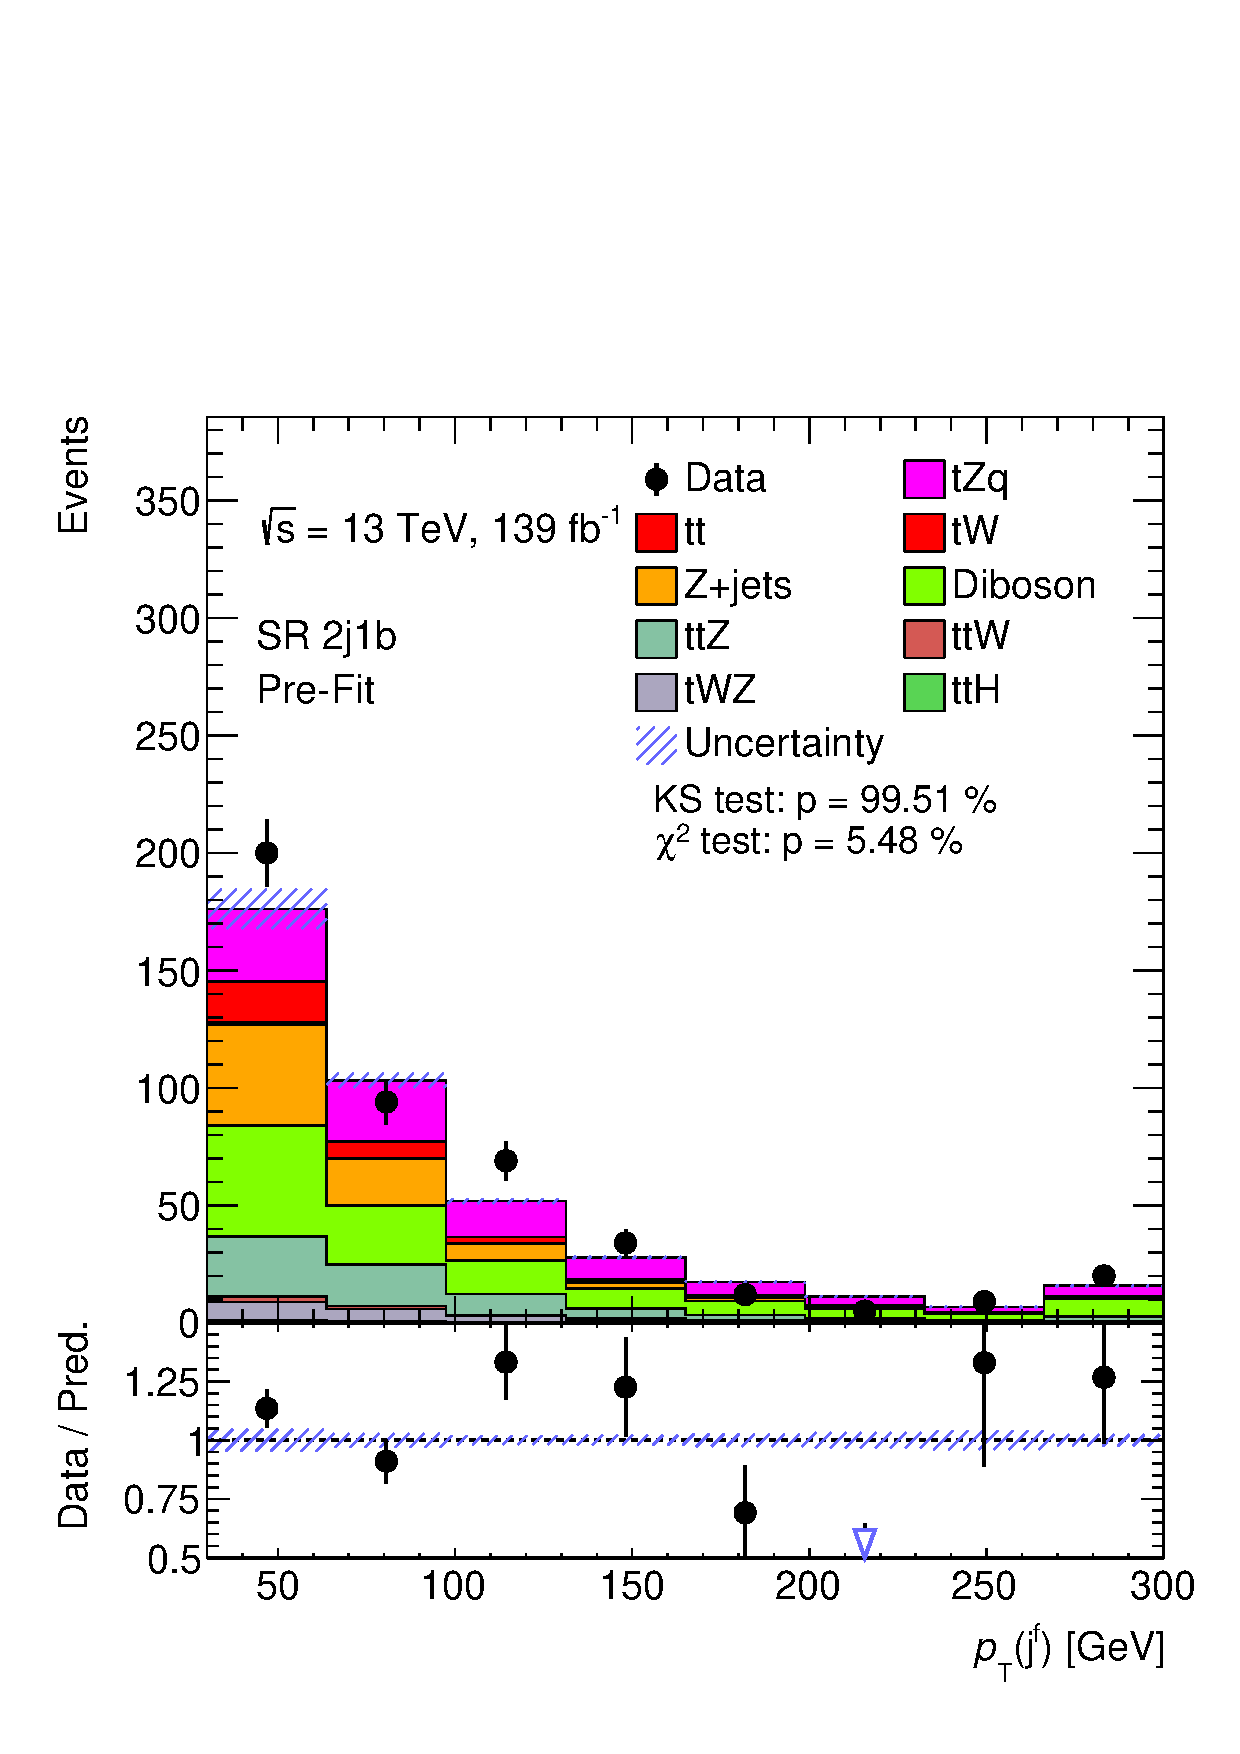
\includegraphics[width=\linewidth]{ubonn-thesis/Chapters/Chapters_06/Figure/Input_distribution/SR_2j1b_forwardjet_pt.pdf} 
  \end{subfigure}%% 
  \begin{subfigure}[b]{0.33\linewidth}
    \centering
    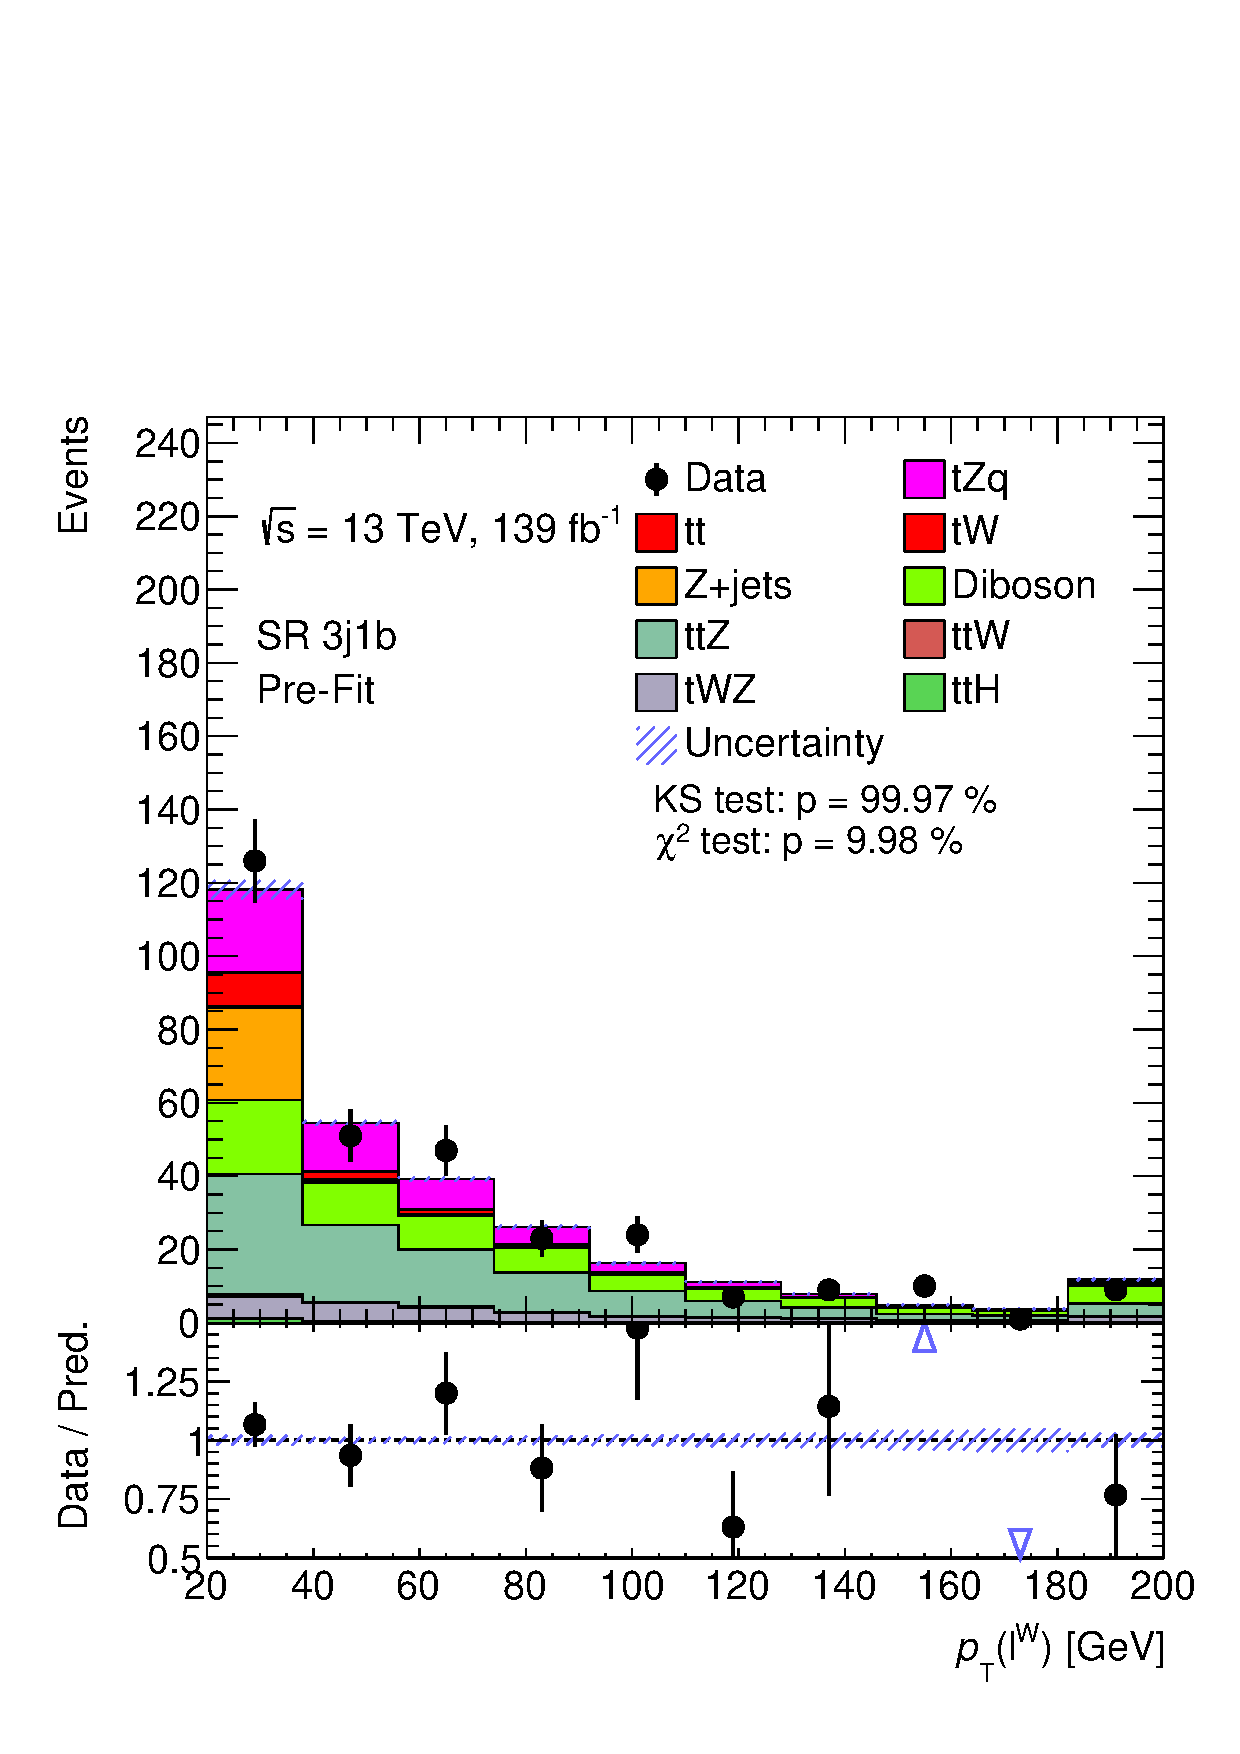
\includegraphics[width=\linewidth]{ubonn-thesis/Chapters/Chapters_06/Figure/Input_distribution/SR_3j1b_lepW_pt.pdf} 
  \end{subfigure} 
  \newline
  \begin{subfigure}[b]{0.33\linewidth}
    \centering
    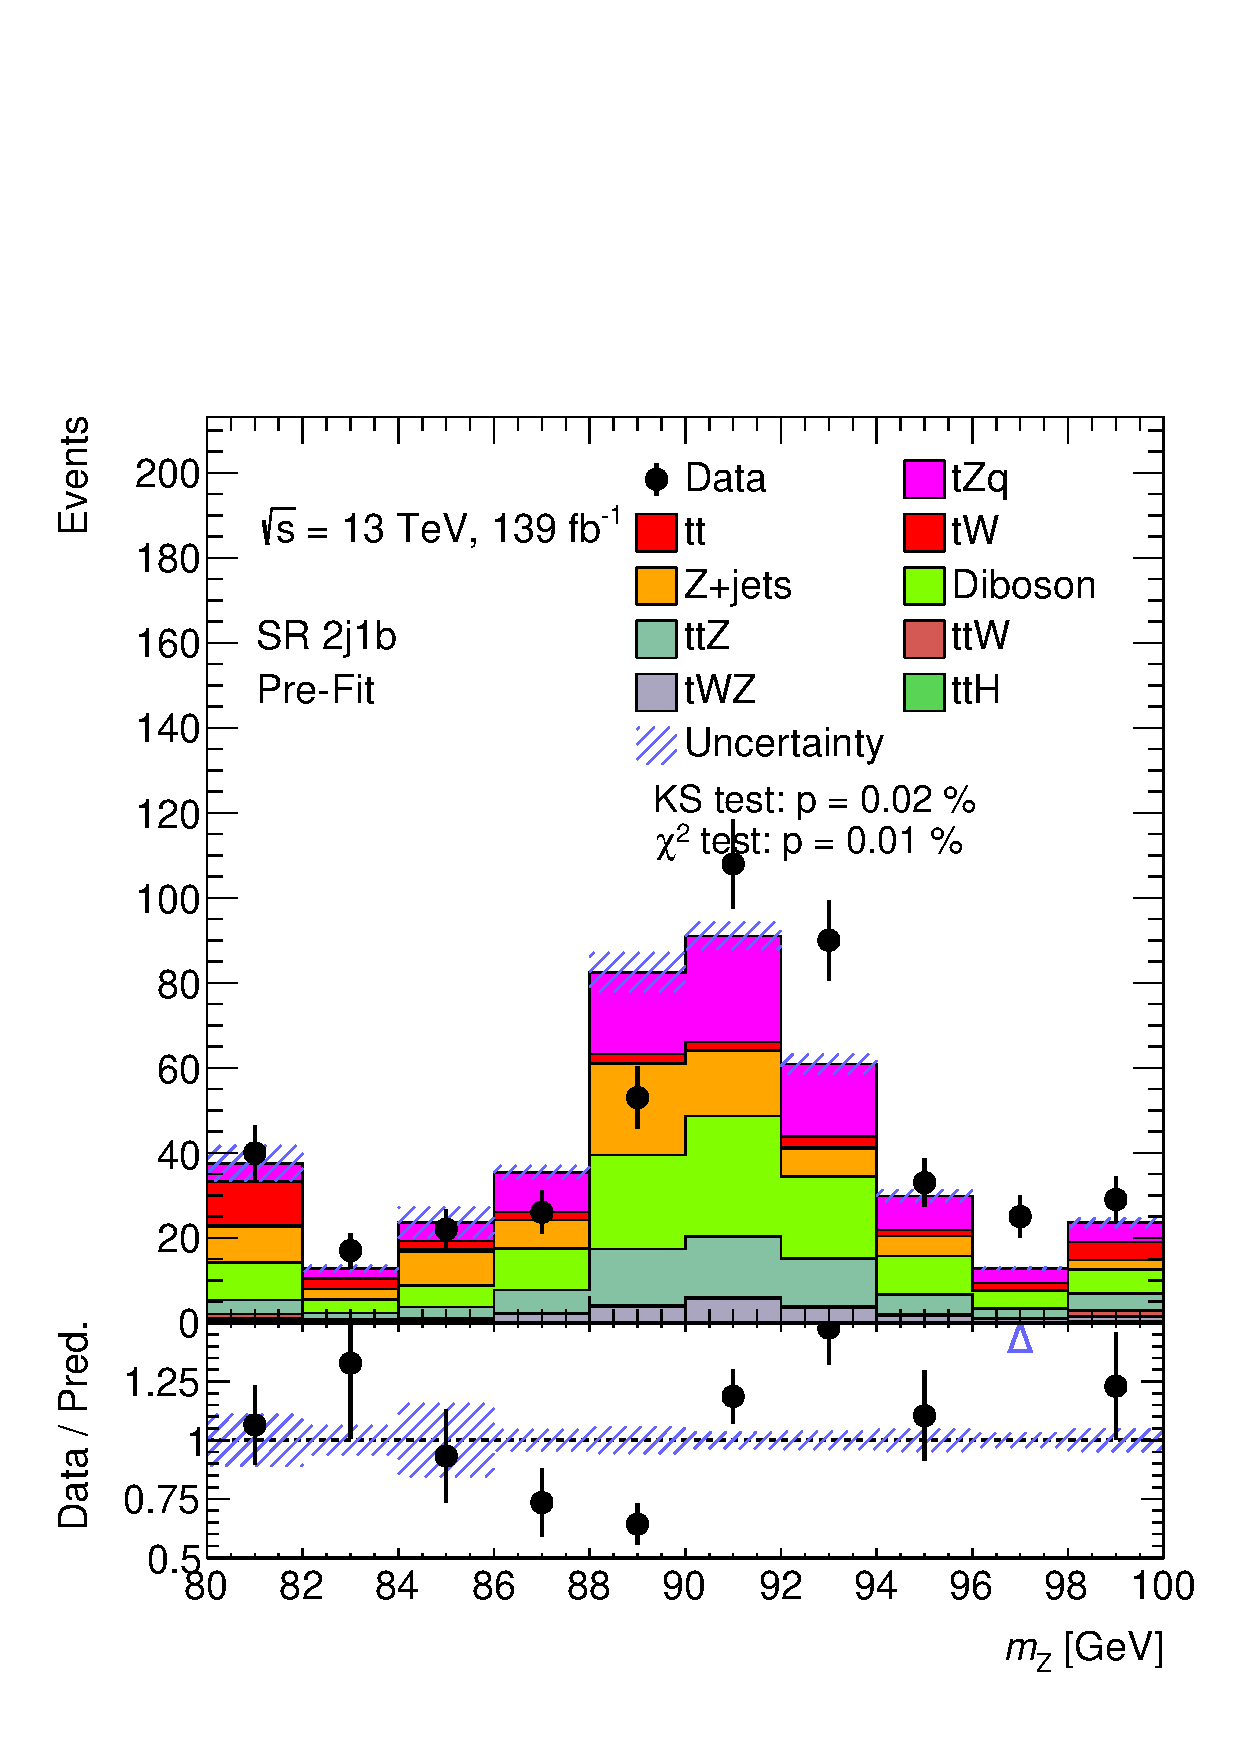
\includegraphics[width=\linewidth]{ubonn-thesis/Chapters/Chapters_06/Figure/Input_distribution/SR_2j1b_MZ.pdf} 
  \end{subfigure}%%
  \begin{subfigure}[b]{0.33\linewidth}
    \centering
    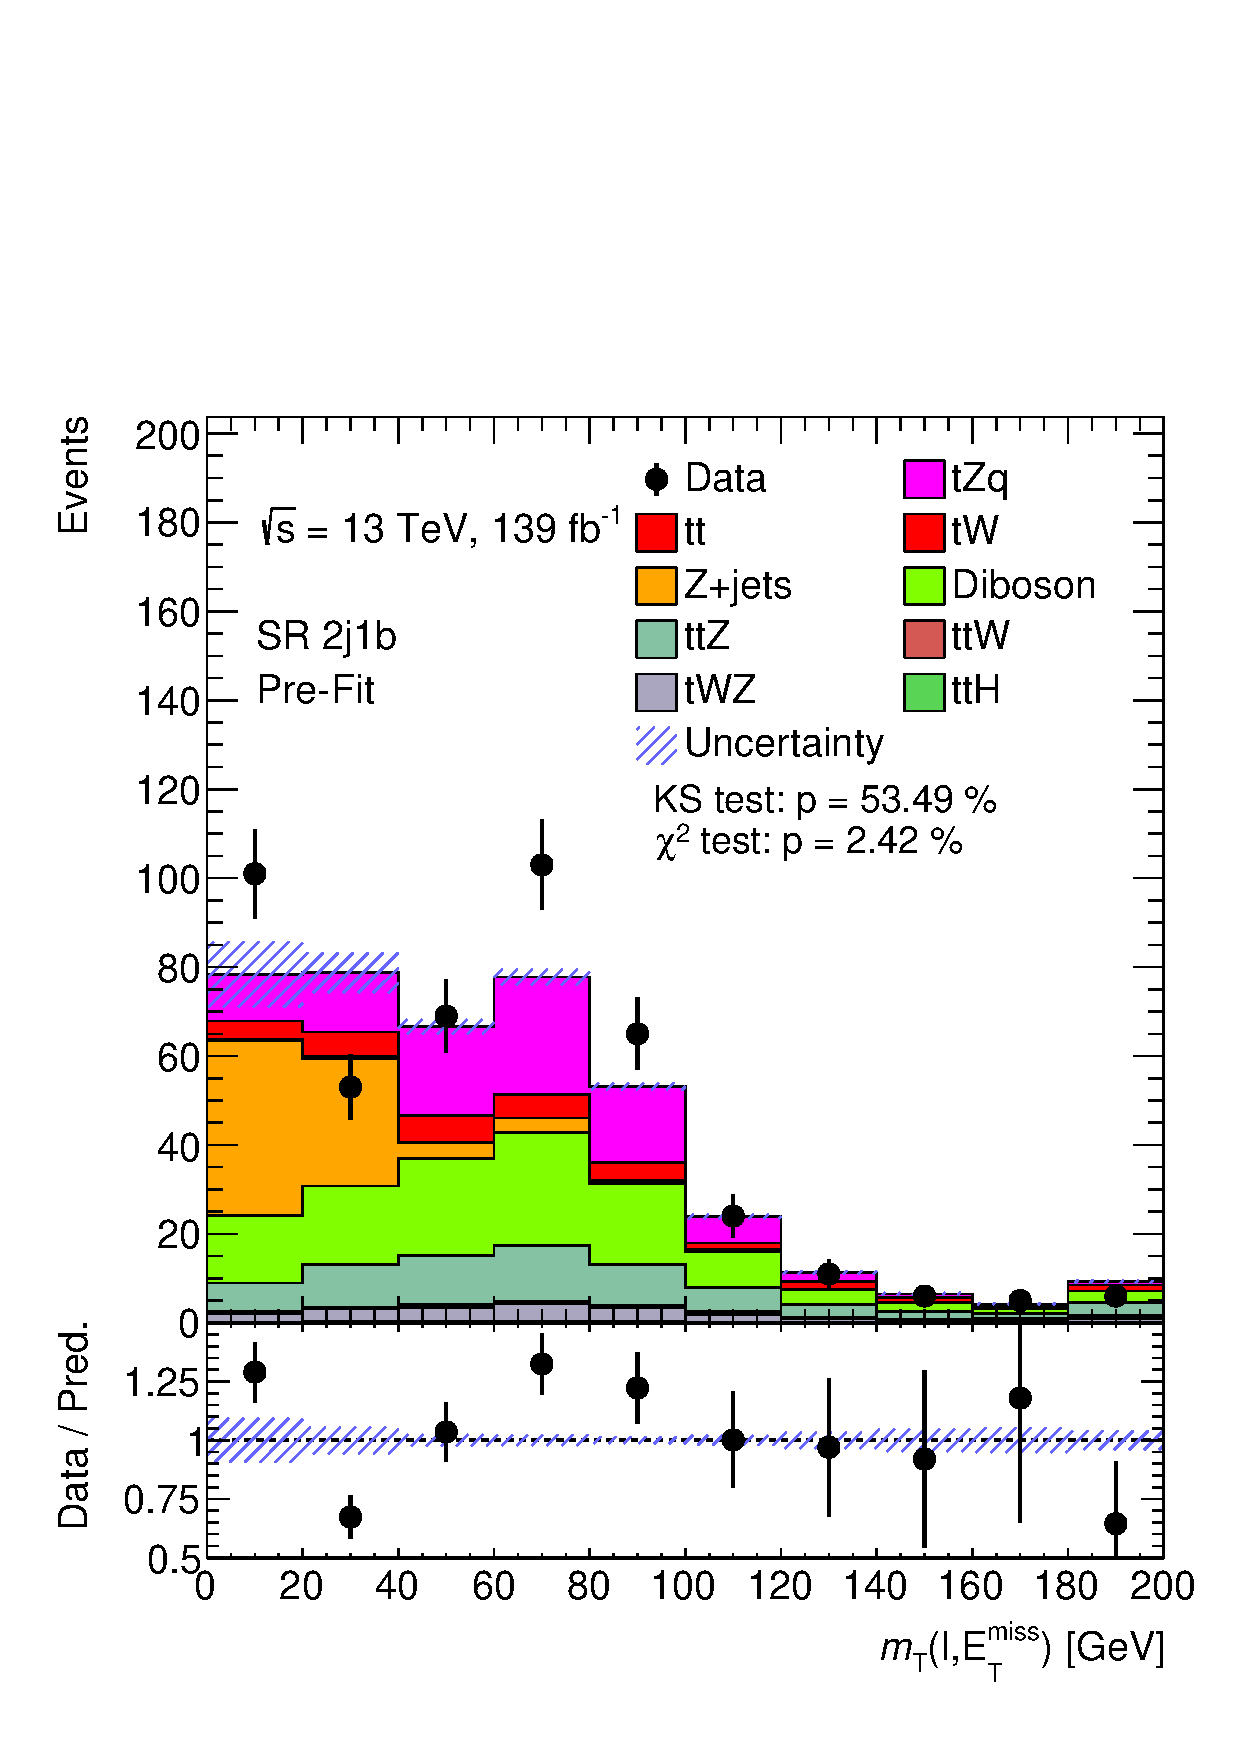
\includegraphics[width=\linewidth]{ubonn-thesis/Chapters/Chapters_06/Figure/Input_distribution/SR_2j1b_mtW.pdf} 
  \end{subfigure}
  \begin{subfigure}[b]{0.33\linewidth}
    \centering
    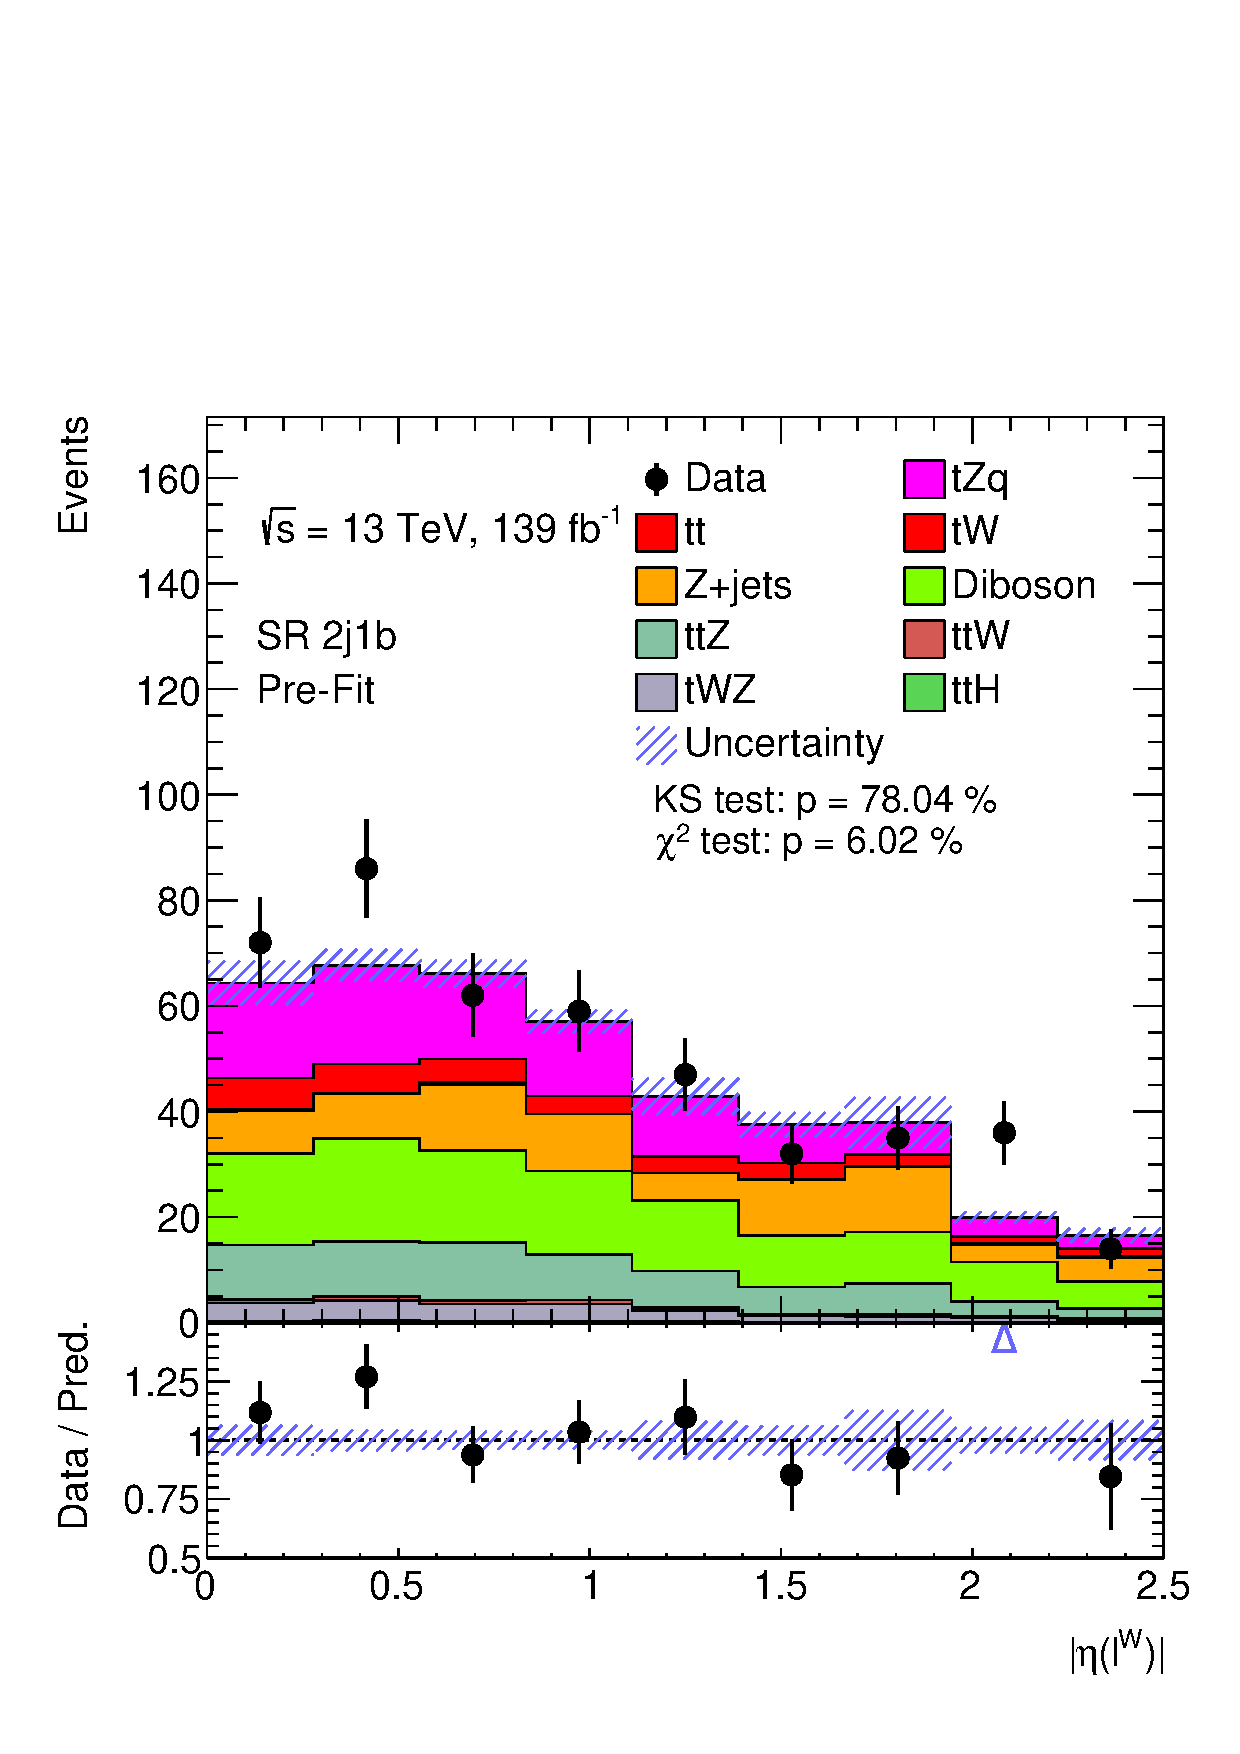
\includegraphics[width=\linewidth]{ubonn-thesis/Chapters/Chapters_06/Figure/Input_distribution/SR_2j1b_lepW_eta.pdf} 
  \end{subfigure} 
  
  \caption{ Stacked kinematic plots of neural-network training variables of the SR 2j1b, in order of significance. Both signal and backgrounds are normalised to the expected number of events before the fit. The uncertainty band includes statistical uncertainties for signal and backgrounds }
  \label{fig_signal1} 
  \end{figure}


\begin{figure}
    \begin{subfigure}[b]{0.32\linewidth}
    \centering
    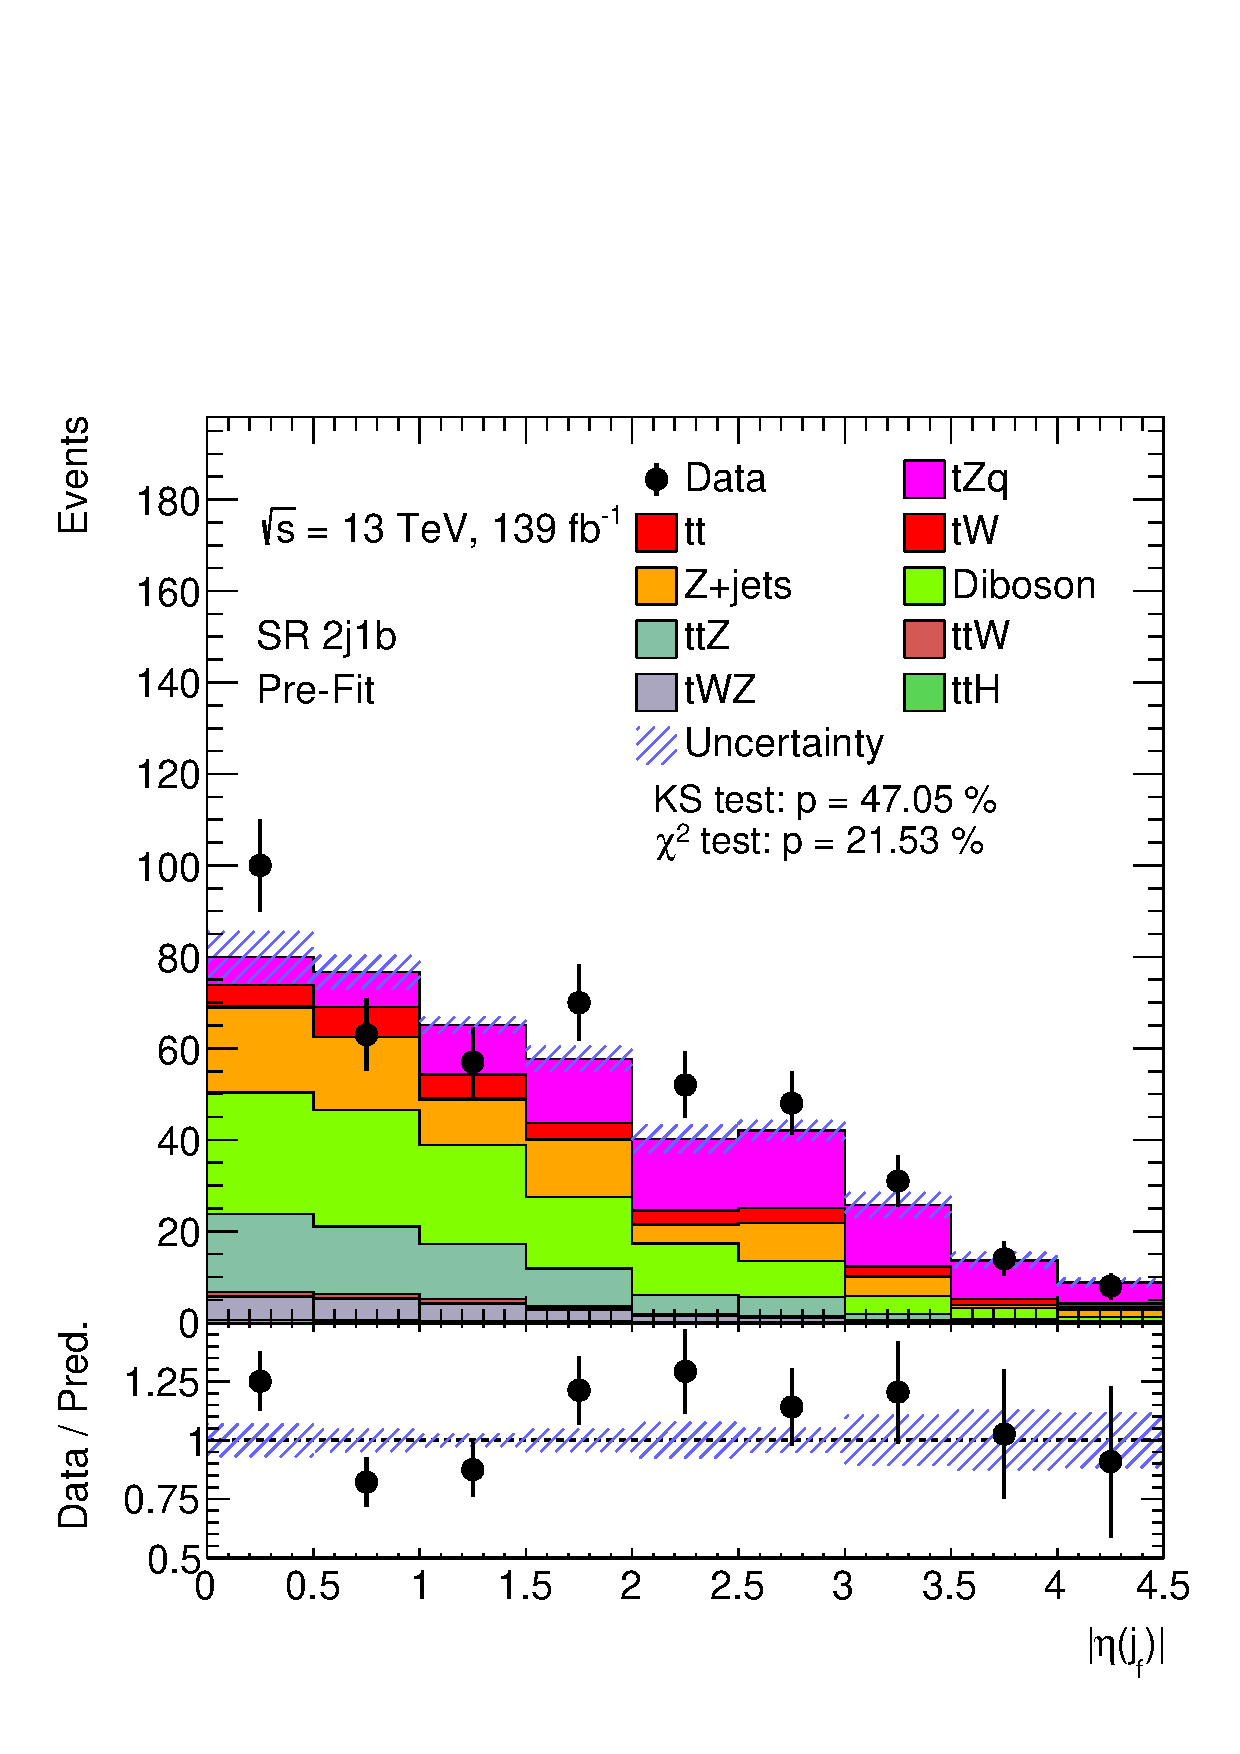
\includegraphics[width=\linewidth]{ubonn-thesis/Chapters/Chapters_06/Figure/Input_distribution/SR_2j1b_forwardjet_eta.pdf} 
  \end{subfigure}%%
  \begin{subfigure}[b]{0.32\linewidth}
    \centering
    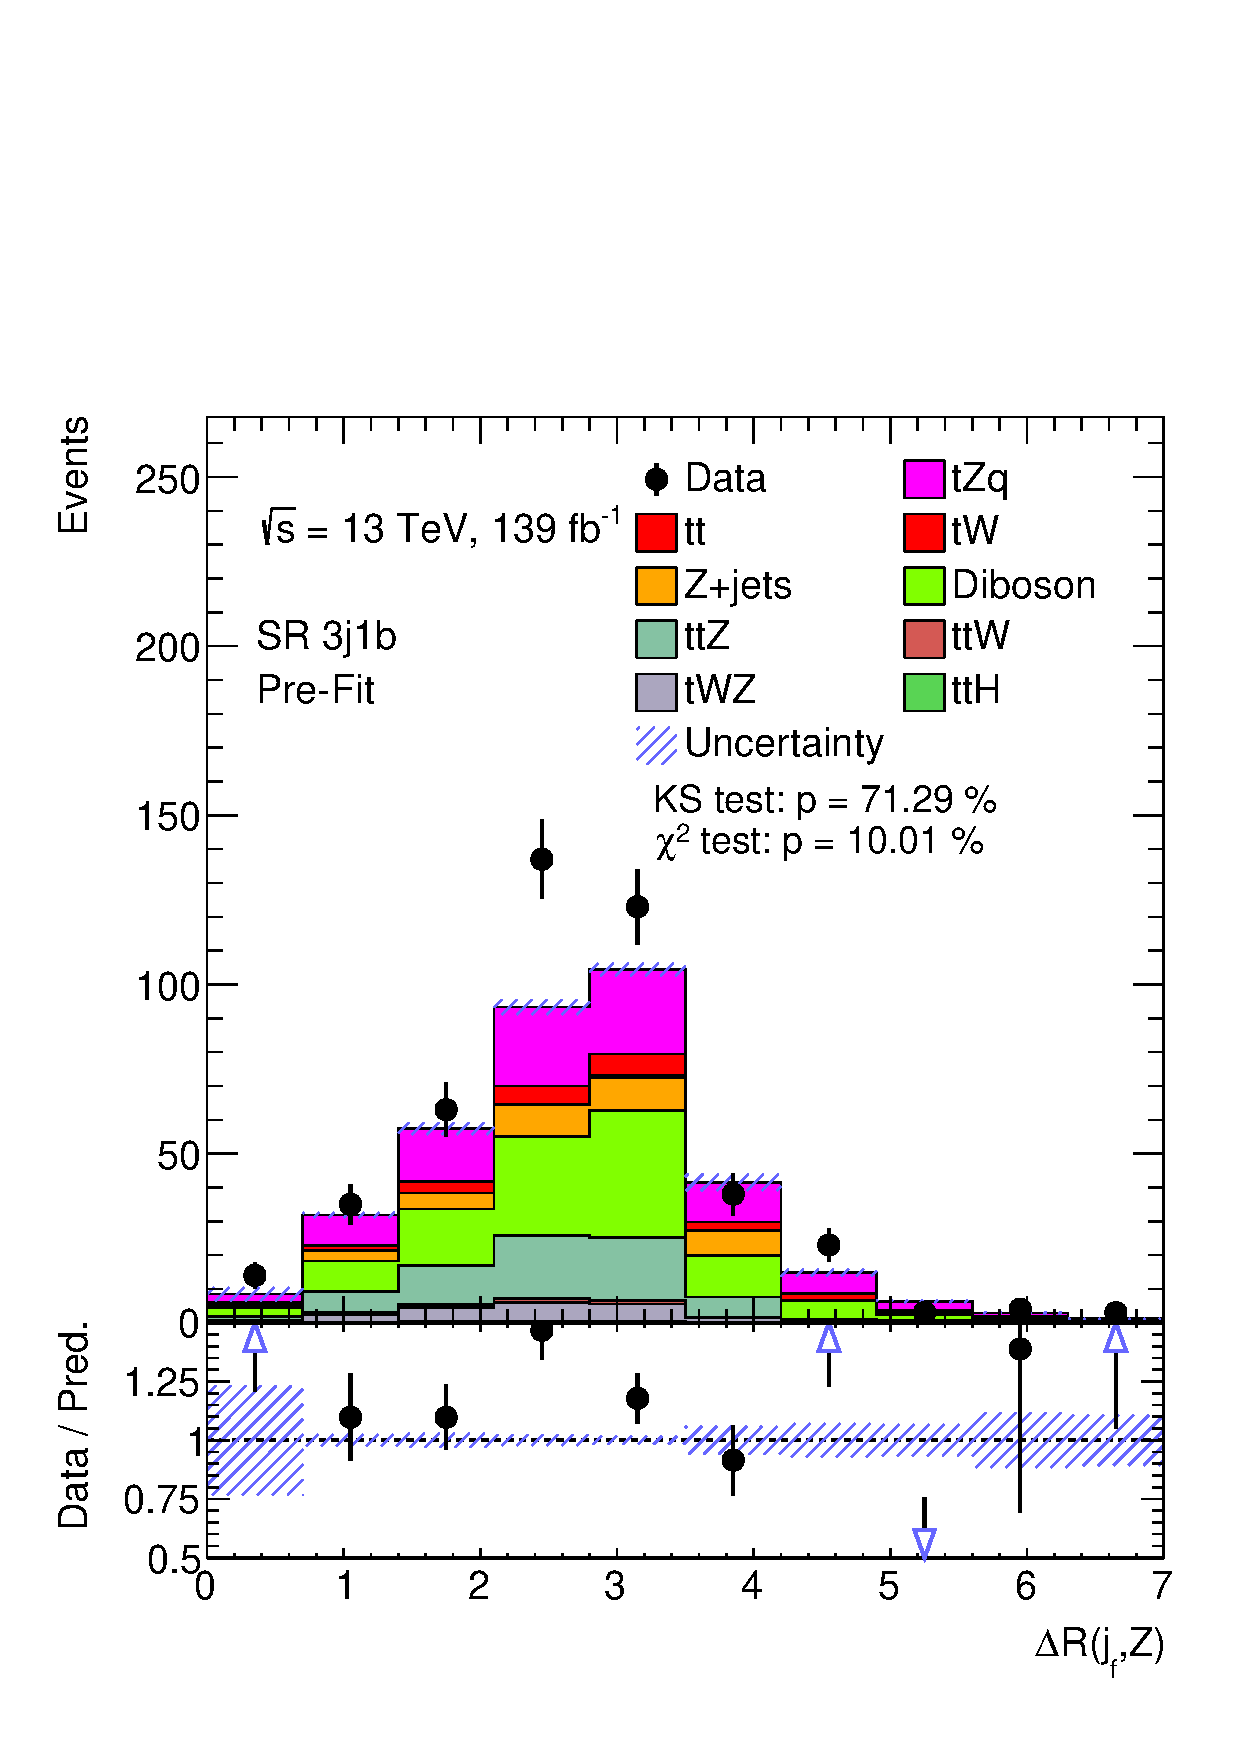
\includegraphics[width=\linewidth]{ubonn-thesis/Chapters/Chapters_06/Figure/Input_distribution/SR_2j1b_dR_jf_Z.pdf} 
  \end{subfigure}
  \begin{subfigure}[b]{0.32\linewidth}
    \centering
    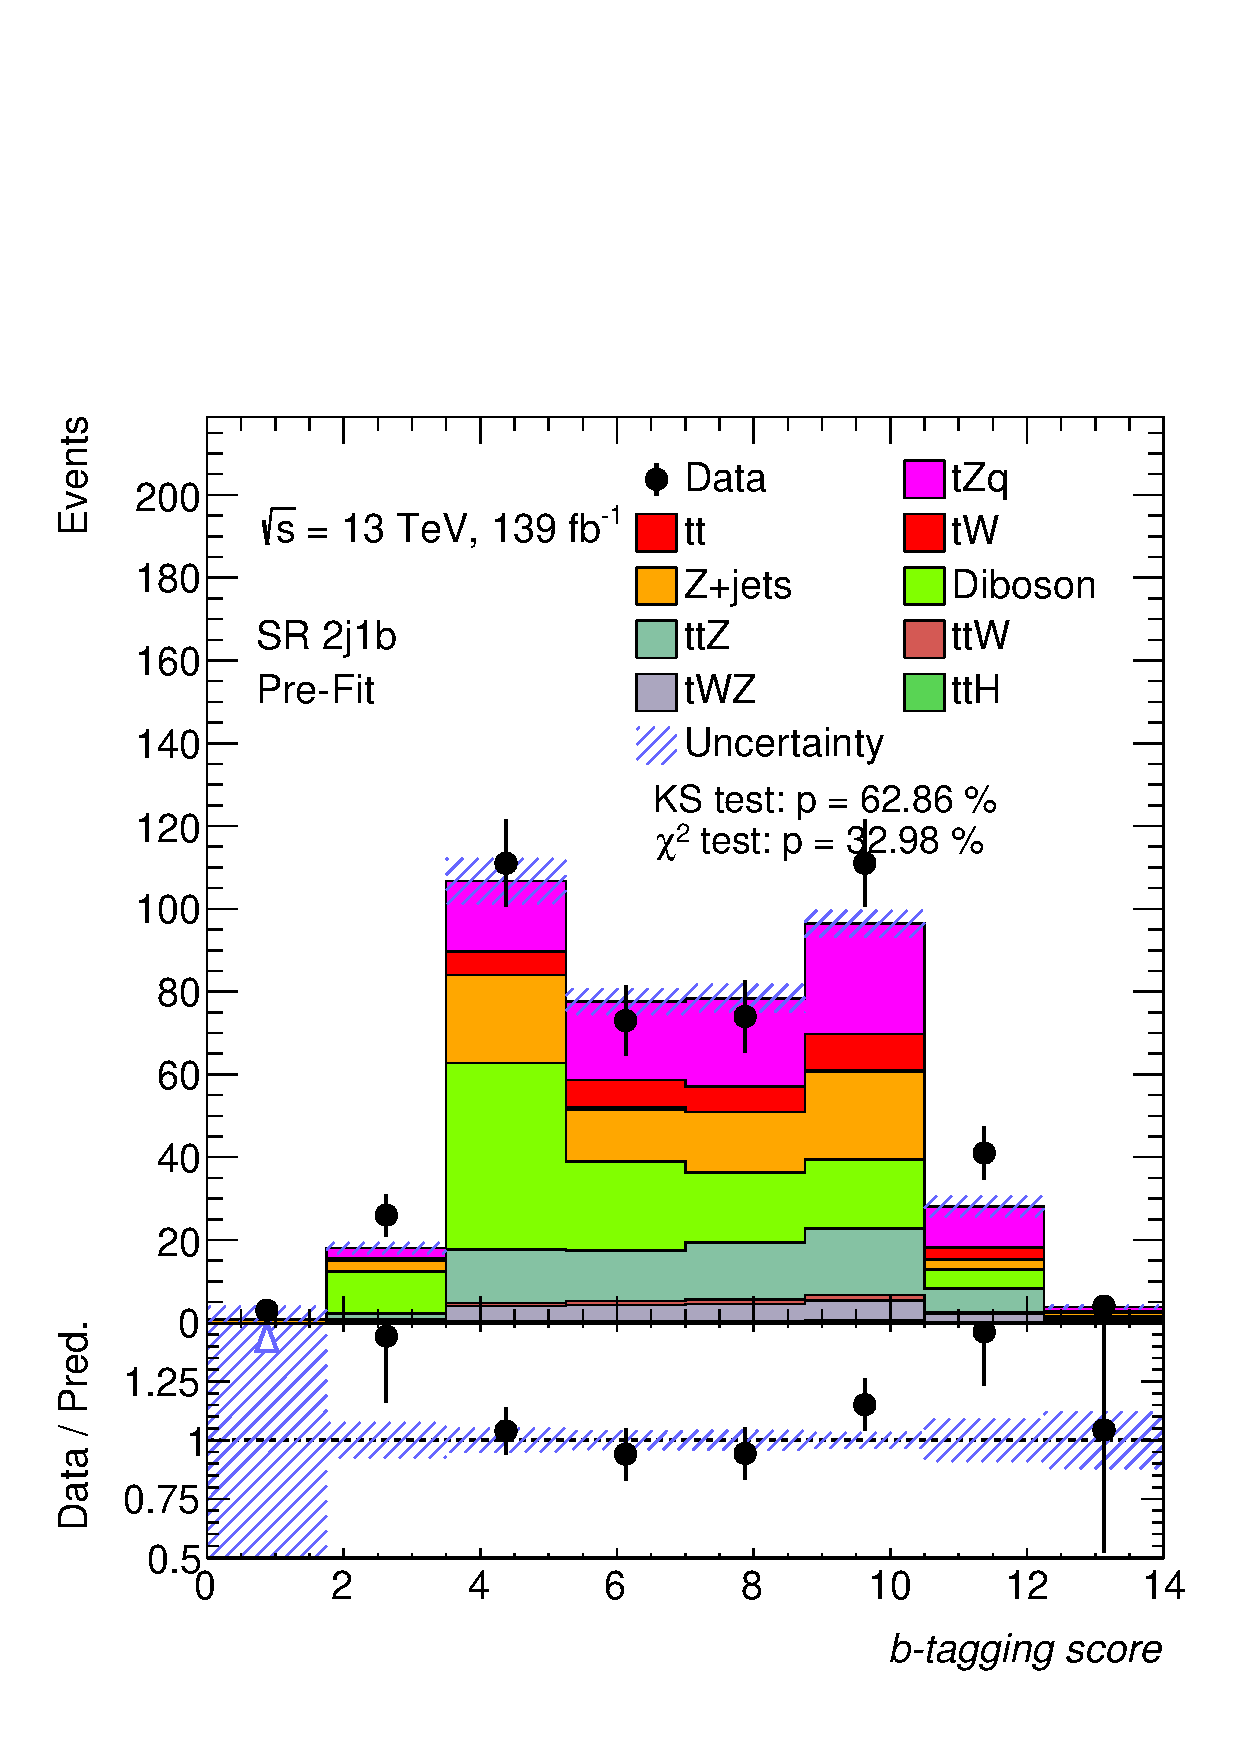
\includegraphics[width=\linewidth]{ubonn-thesis/Chapters/Chapters_06/Figure/Input_distribution/SR_2j1b_btag.pdf} 
  \end{subfigure} 
  \newline
  \centering
  \begin{subfigure}[b]{0.32\linewidth}
    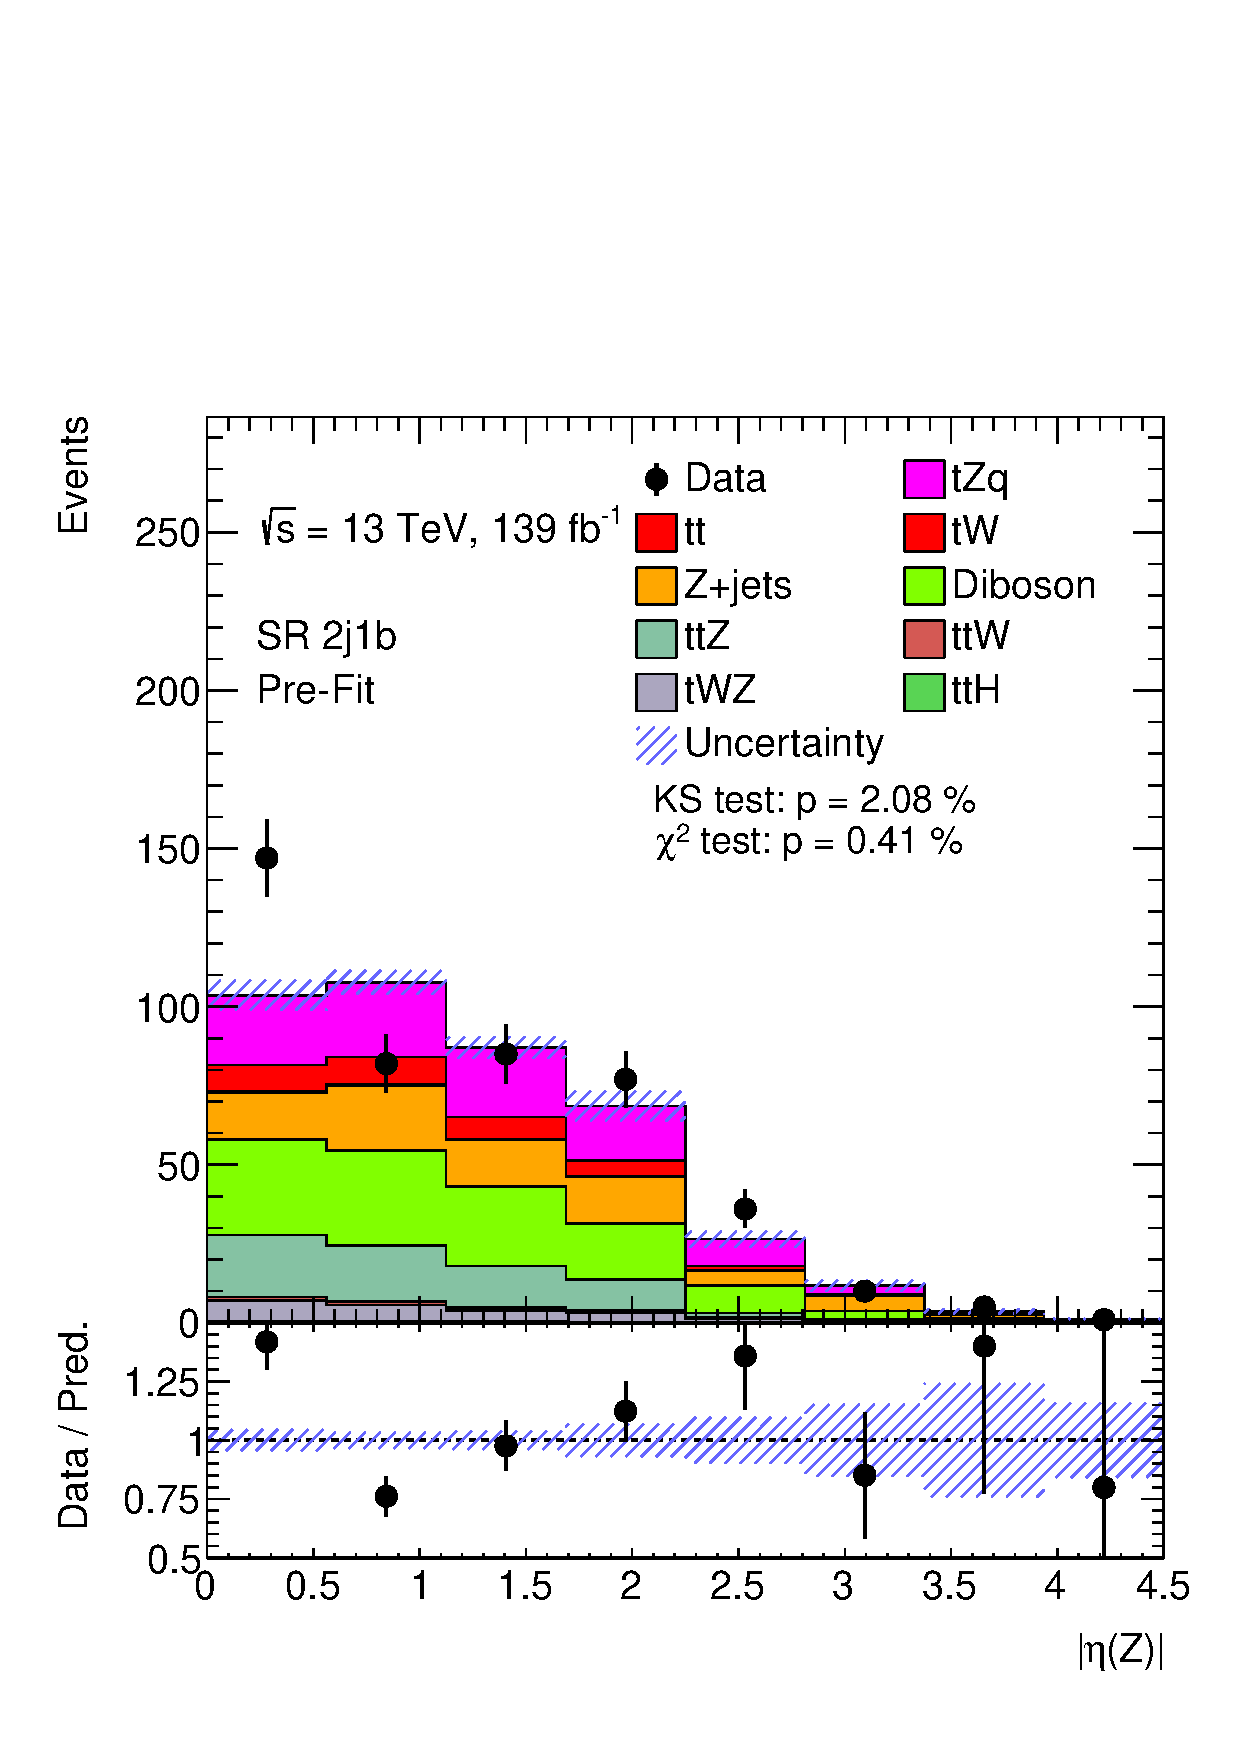
\includegraphics[width=\linewidth]{ubonn-thesis/Chapters/Chapters_06/Figure/Input_distribution/SR_2j1b_Z_eta.pdf} 
  \end{subfigure}%% 
  \hspace*{0.3cm}
  \centering
  \begin{subfigure}[b]{0.32\linewidth}
    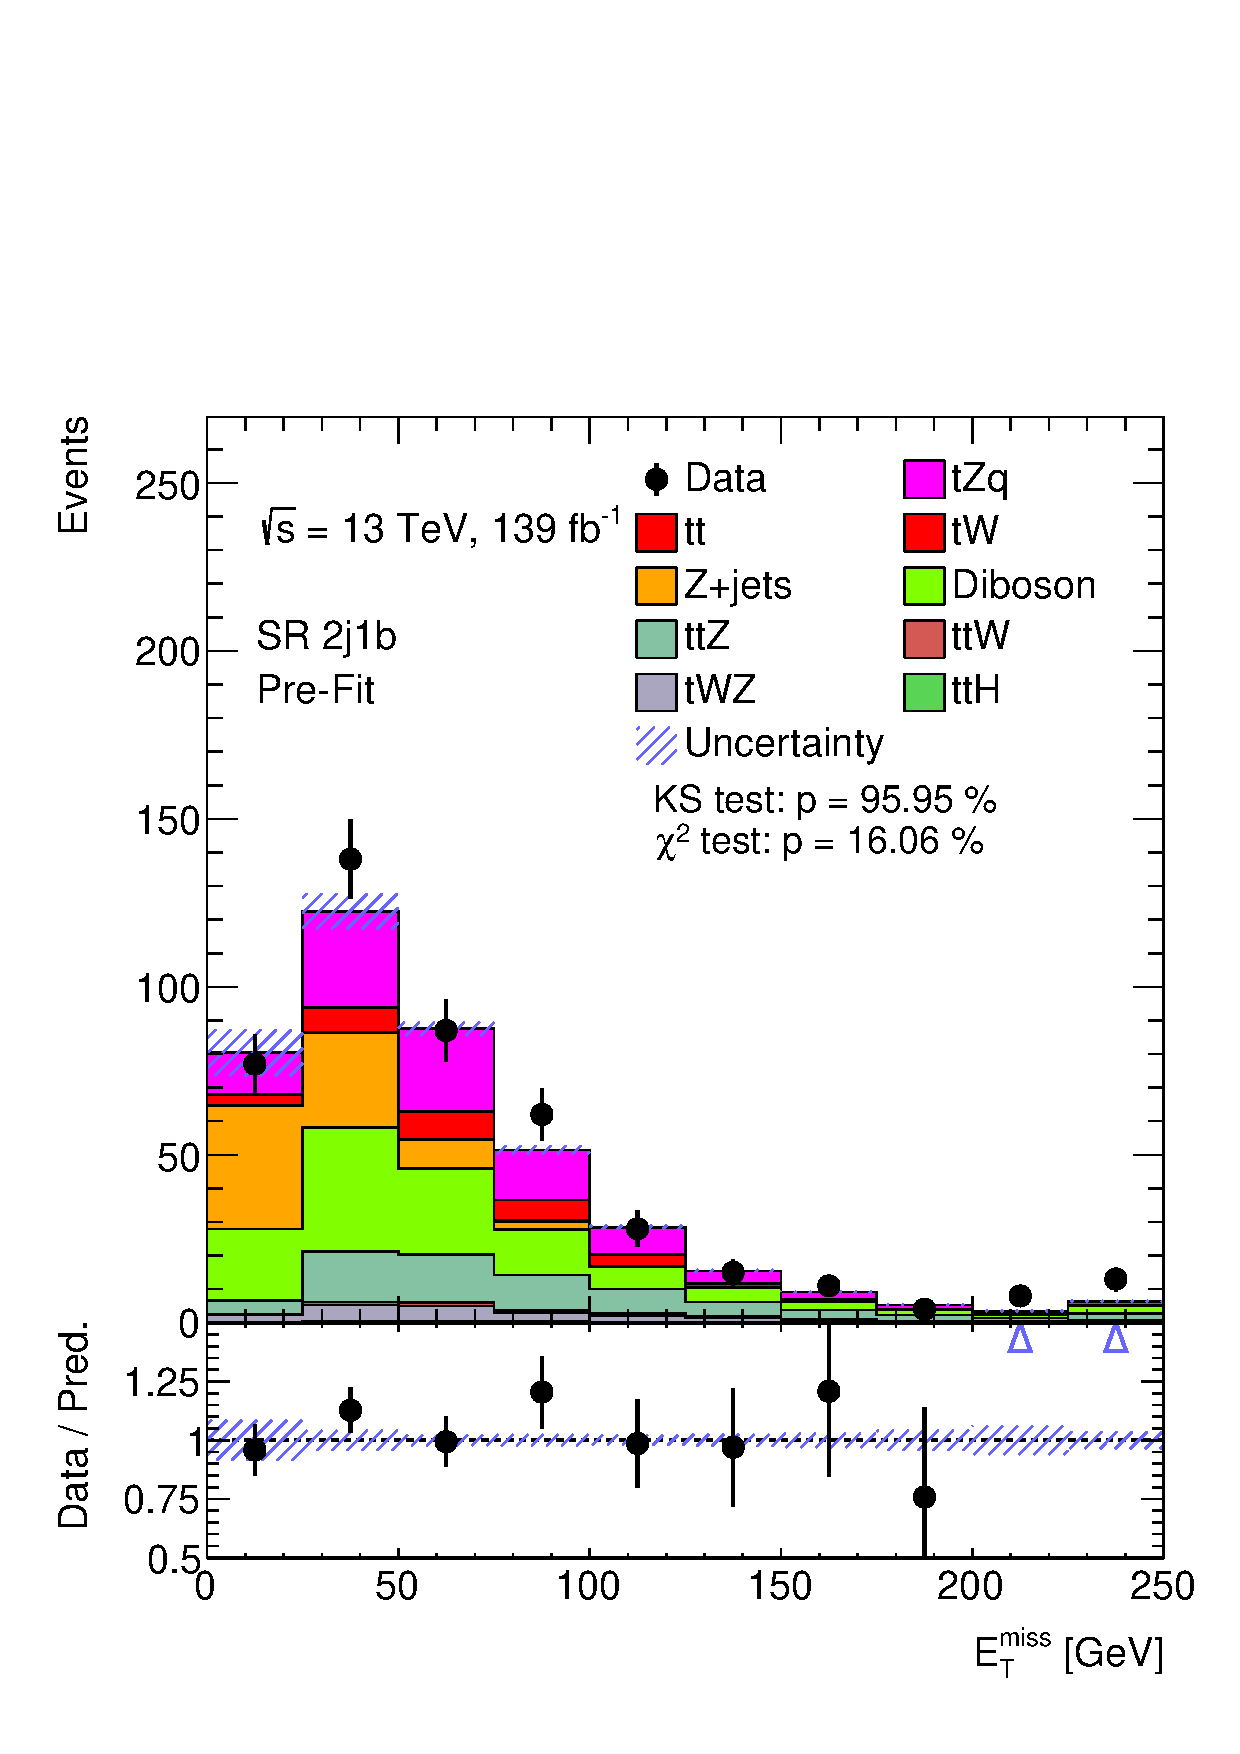
\includegraphics[width=\linewidth]{ubonn-thesis/Chapters/Chapters_06/Figure/Input_distribution/SR_2j1b_MissEt.pdf} 
  \end{subfigure} 
  \caption{Stacked kinematic plots of neural-network training variables of the SR 2j1b, in order of significance. Both signal and backgrounds are normalised to the expected number of events before the fit. The uncertainty band includes statistical uncertainties for signal and backgrounds}
  \label{fig_signal2} 
\end{figure}
%% delta R and pt of forward jet

%% SR 3j1b
\begin{figure}[!h] 
  \begin{subfigure}[b]{0.32\linewidth}
    \centering
    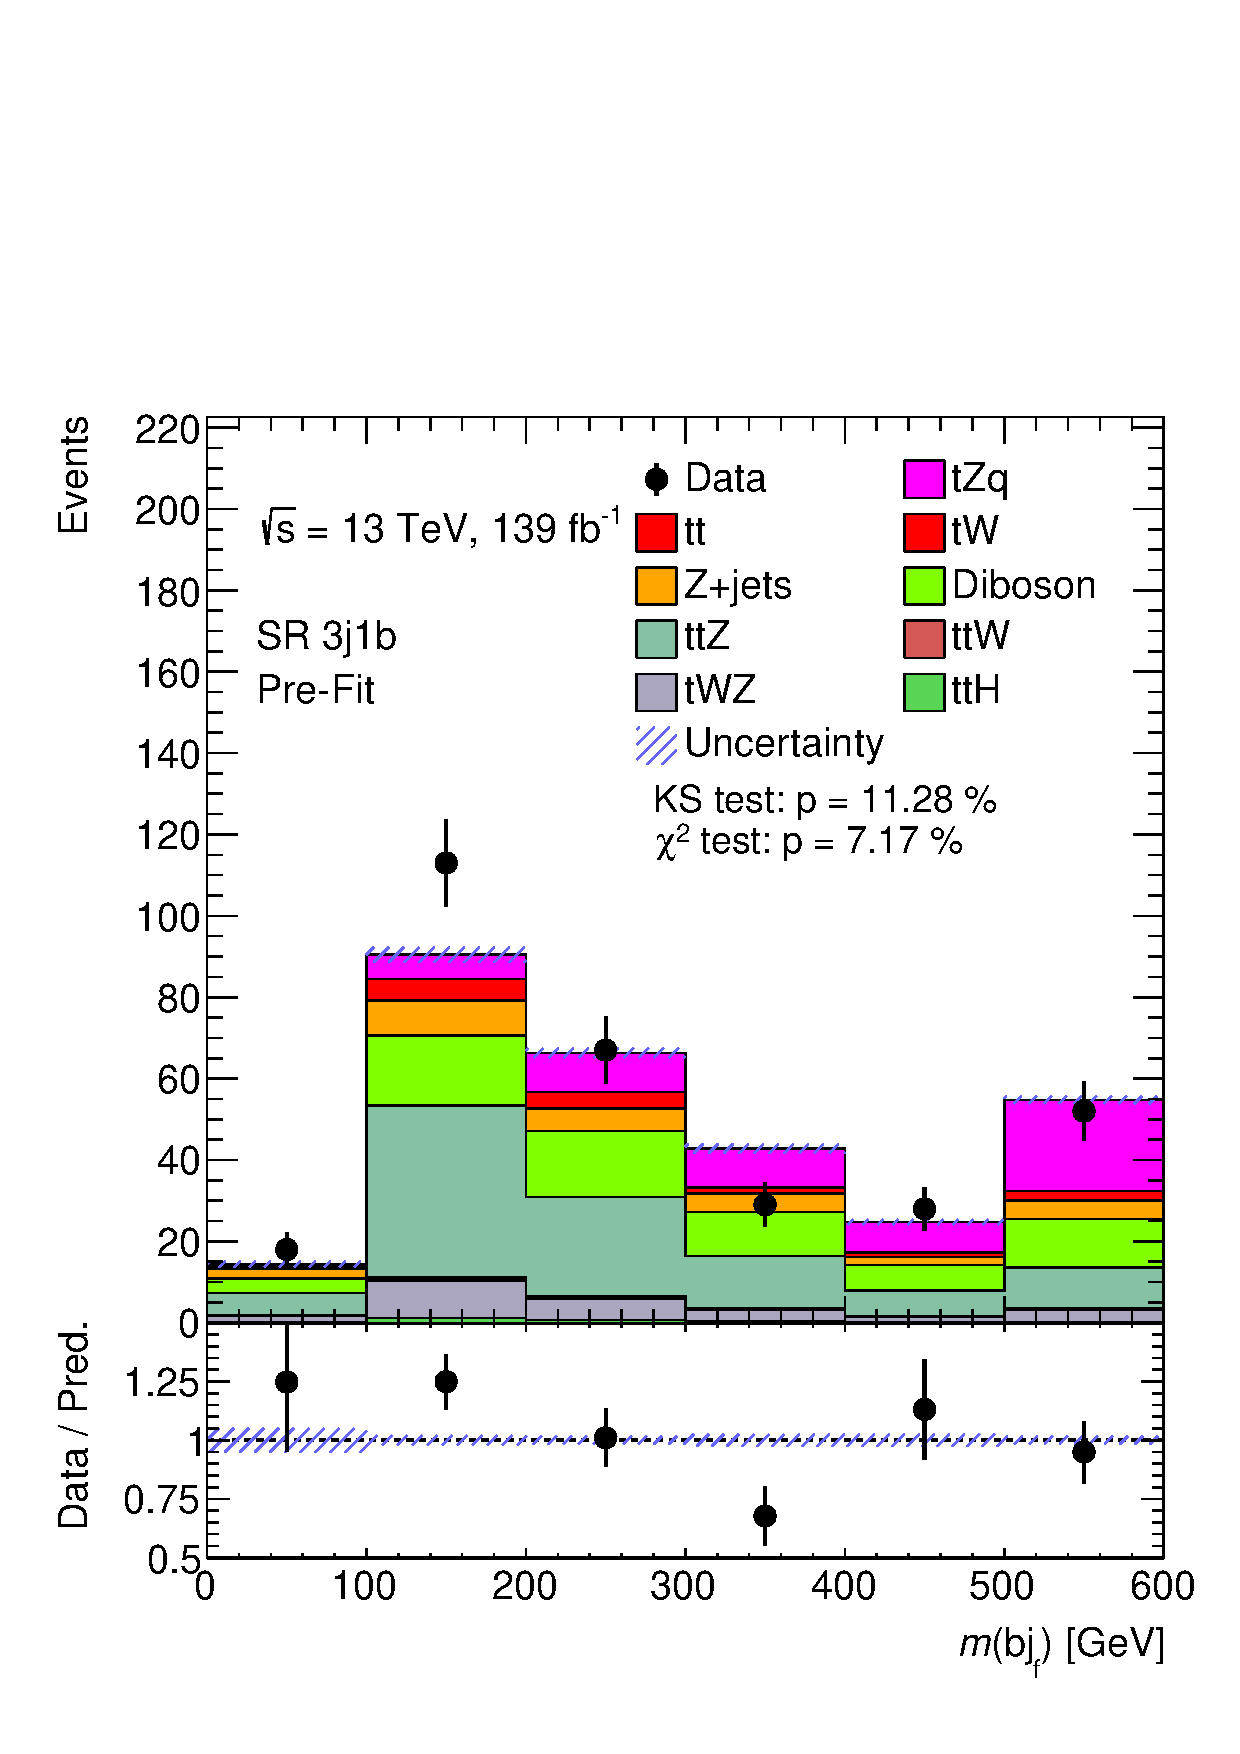
\includegraphics[width=\linewidth]{ubonn-thesis/Chapters/Chapters_06/Figure/Input_distribution/SR_3j1b_M_bj.pdf} 
  \end{subfigure}%% 
  \begin{subfigure}[b]{0.32\linewidth}
    \centering
    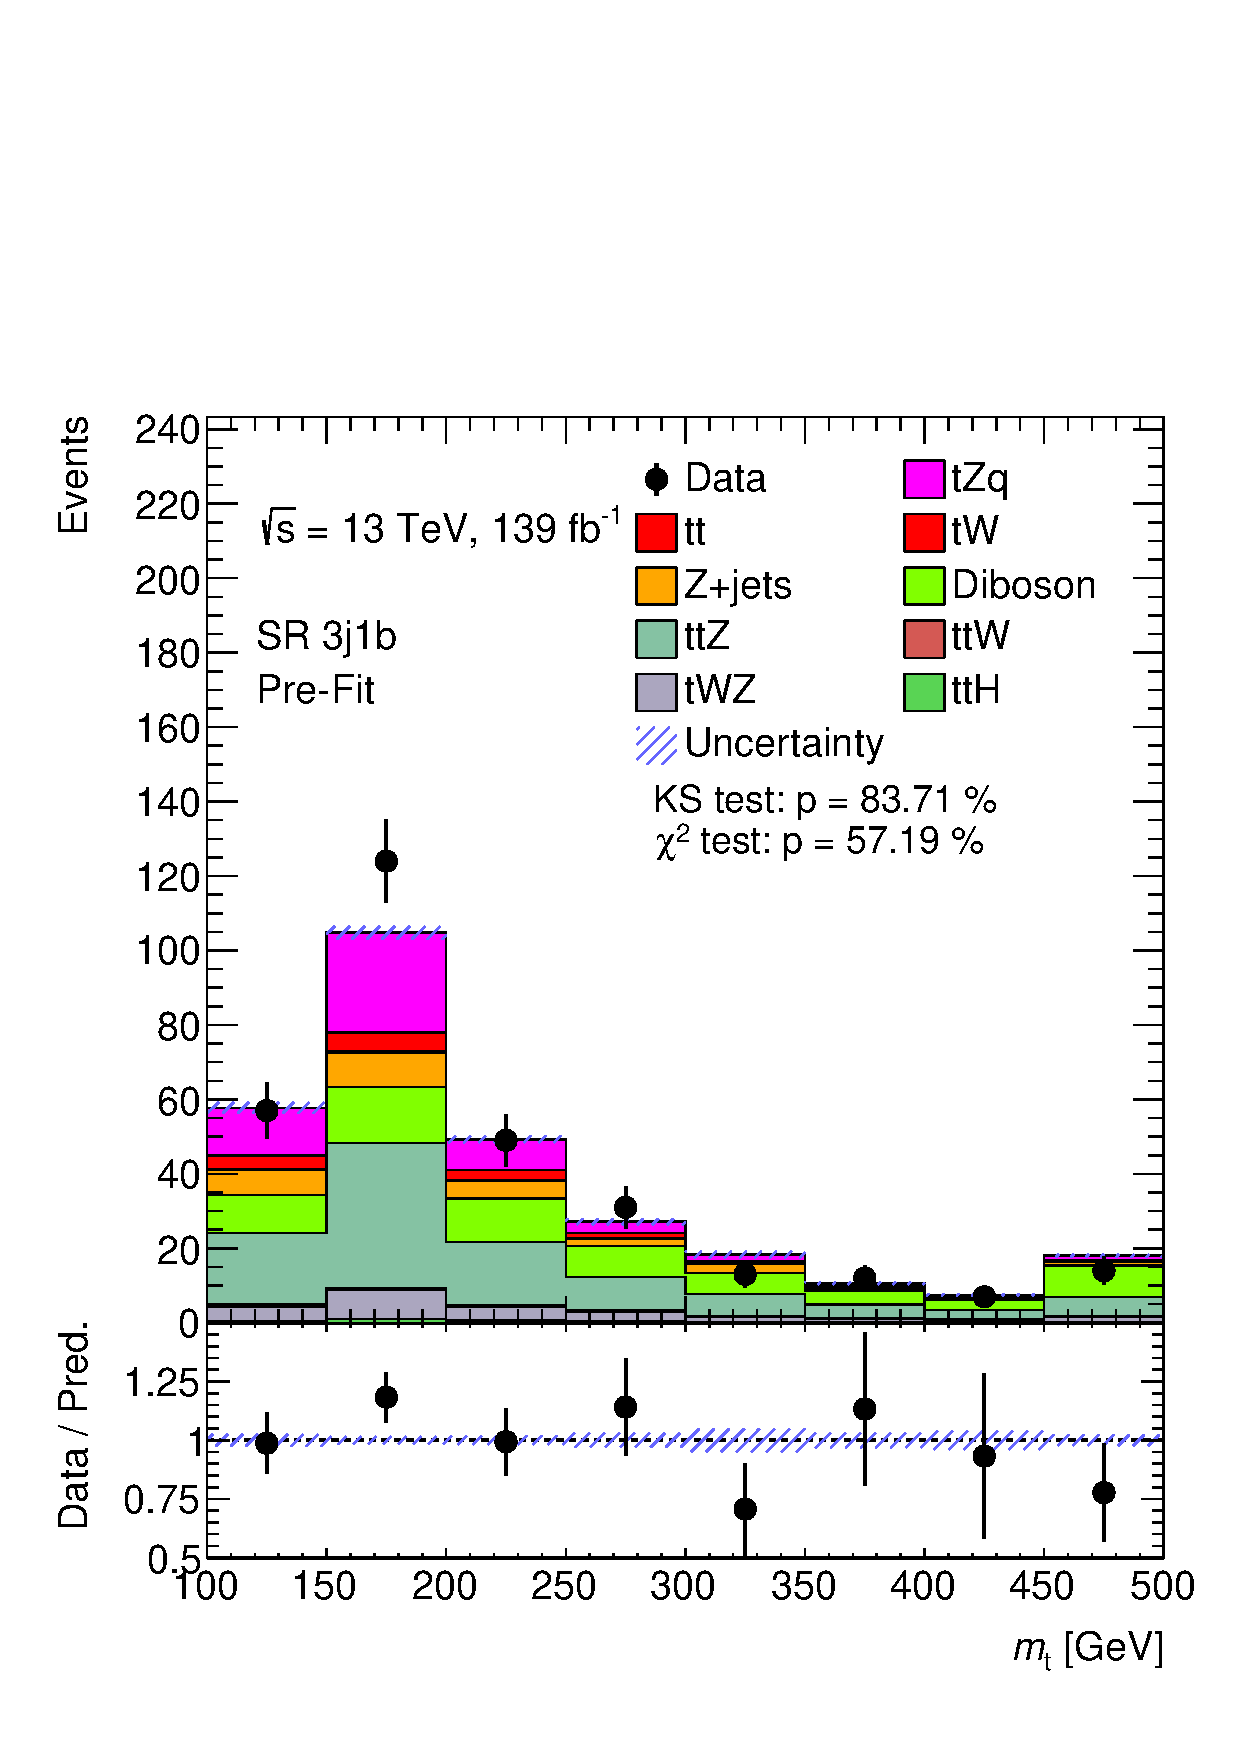
\includegraphics[width=\linewidth]{ubonn-thesis/Chapters/Chapters_06/Figure/Input_distribution/SR_3j1b_Top_mass.pdf} 
  \end{subfigure} 
  \begin{subfigure}[b]{0.32\linewidth}
    \centering
    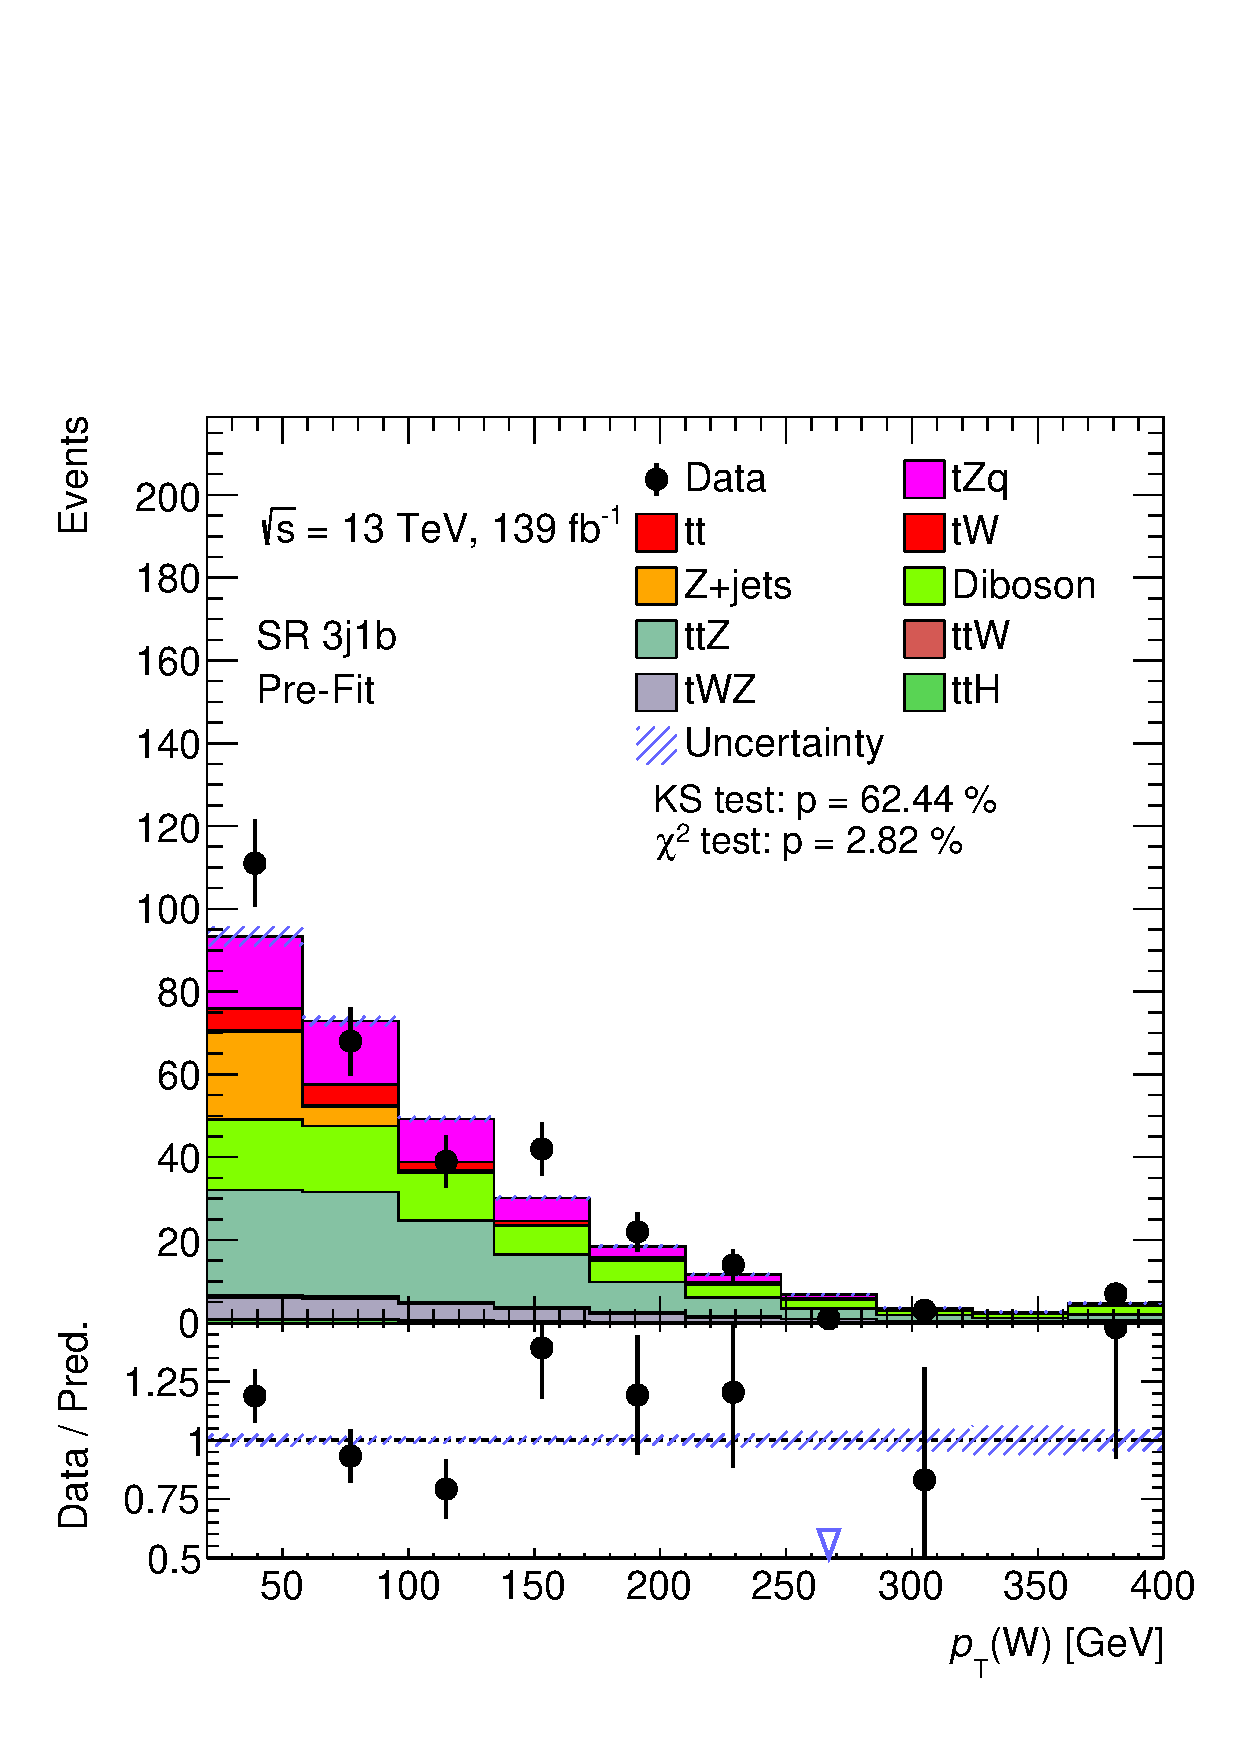
\includegraphics[width=\linewidth]{ubonn-thesis/Chapters/Chapters_06/Figure/Input_distribution/SR_3j1b_W_pt.pdf} 
  \end{subfigure}%%
  \caption{Stacked kinematic plots of neural-network training variables of the SR 3j1b, in order of significance. Both signal and backgrounds are normalised to the expected number of events before the fit. The uncertainty band includes statistical uncertainties for signal and backgrounds}
  \label{fig_signal3}
  \end{figure}


\begin{figure}[!h] 
\vspace*{0.4cm}
  \begin{subfigure}[b]{0.33\linewidth}
    \centering
    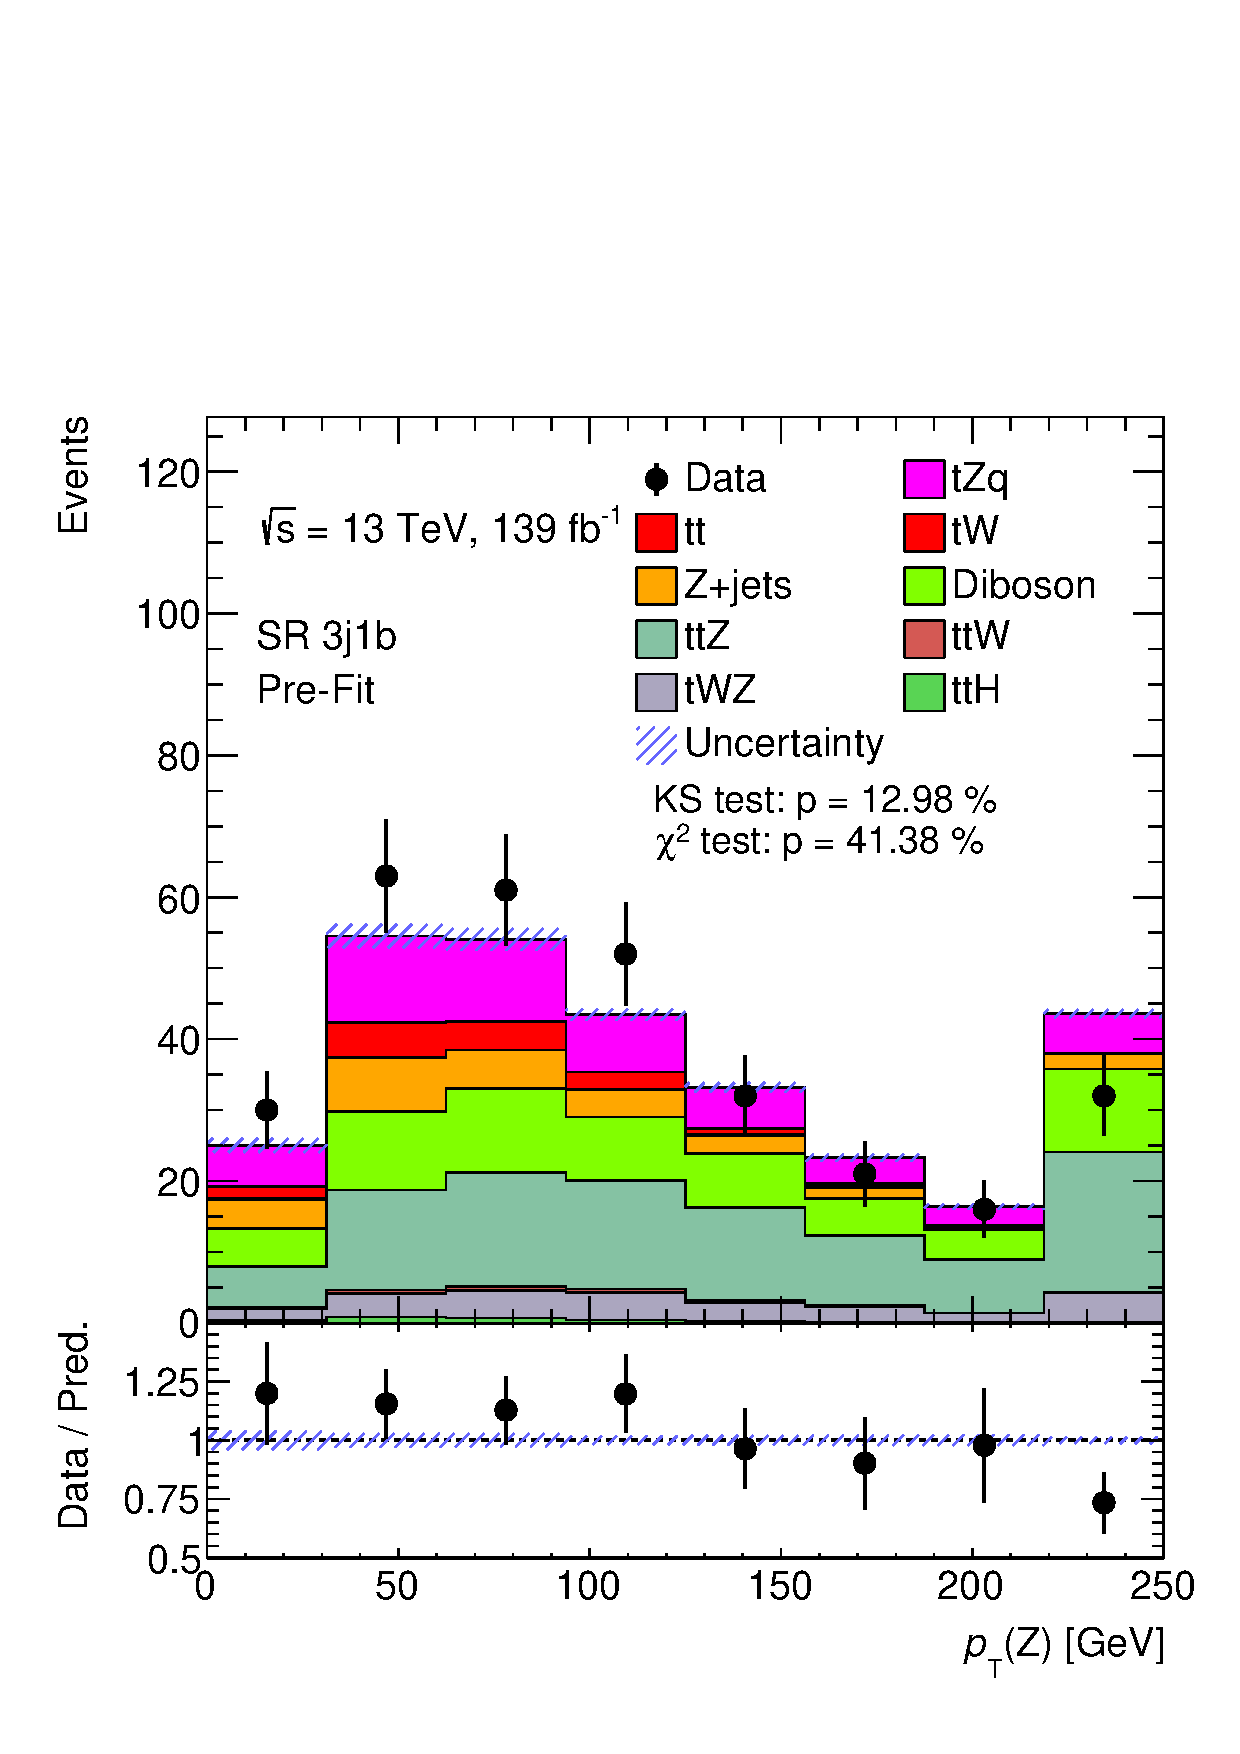
\includegraphics[width=\linewidth]{ubonn-thesis/Chapters/Chapters_06/Figure/Input_distribution/SR_3j1b_Z_pt.pdf} 
  \end{subfigure} 
  \begin{subfigure}[b]{0.33\linewidth}
    \centering
    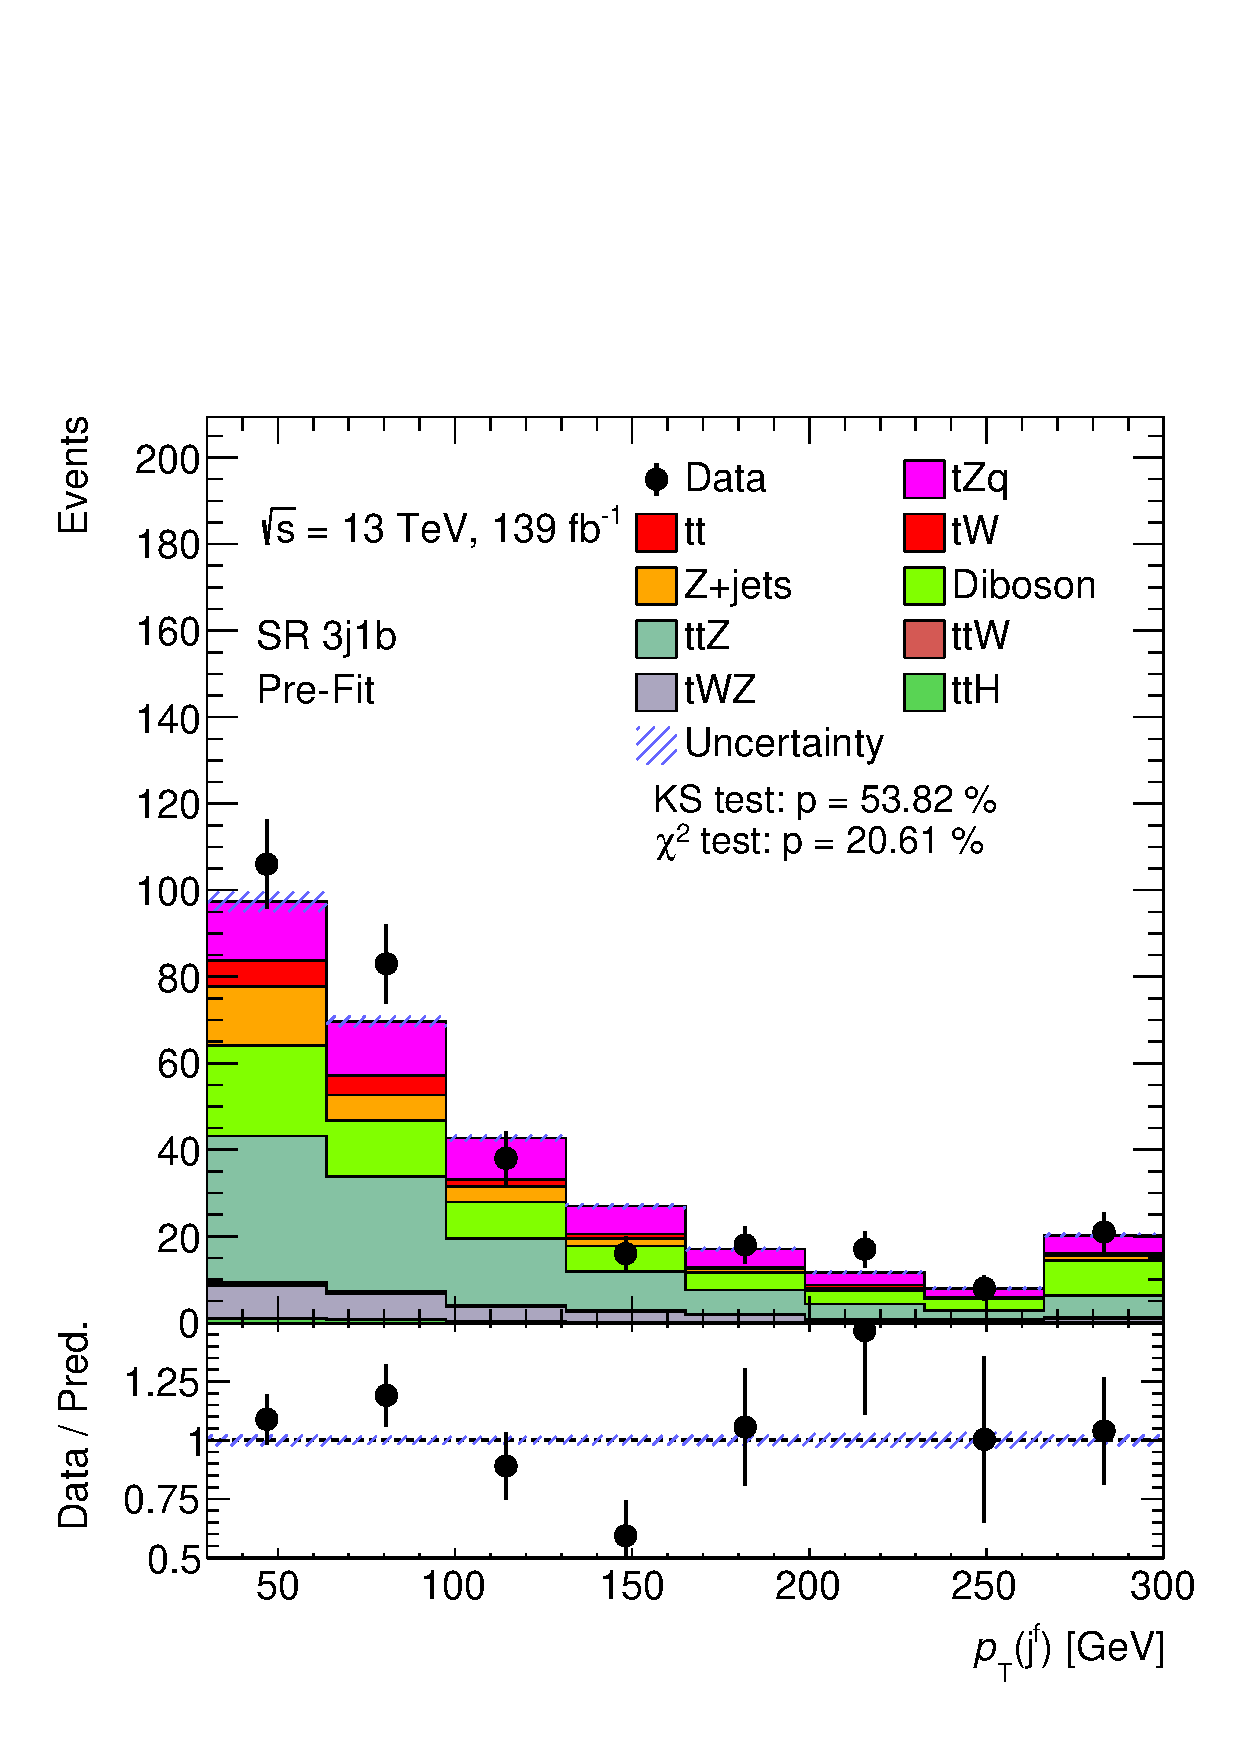
\includegraphics[width=\linewidth]{ubonn-thesis/Chapters/Chapters_06/Figure/Input_distribution/SR_3j1b_forwardjet_pt.pdf} 
  \end{subfigure}%% 
  \begin{subfigure}[b]{0.33\linewidth}
    \centering
    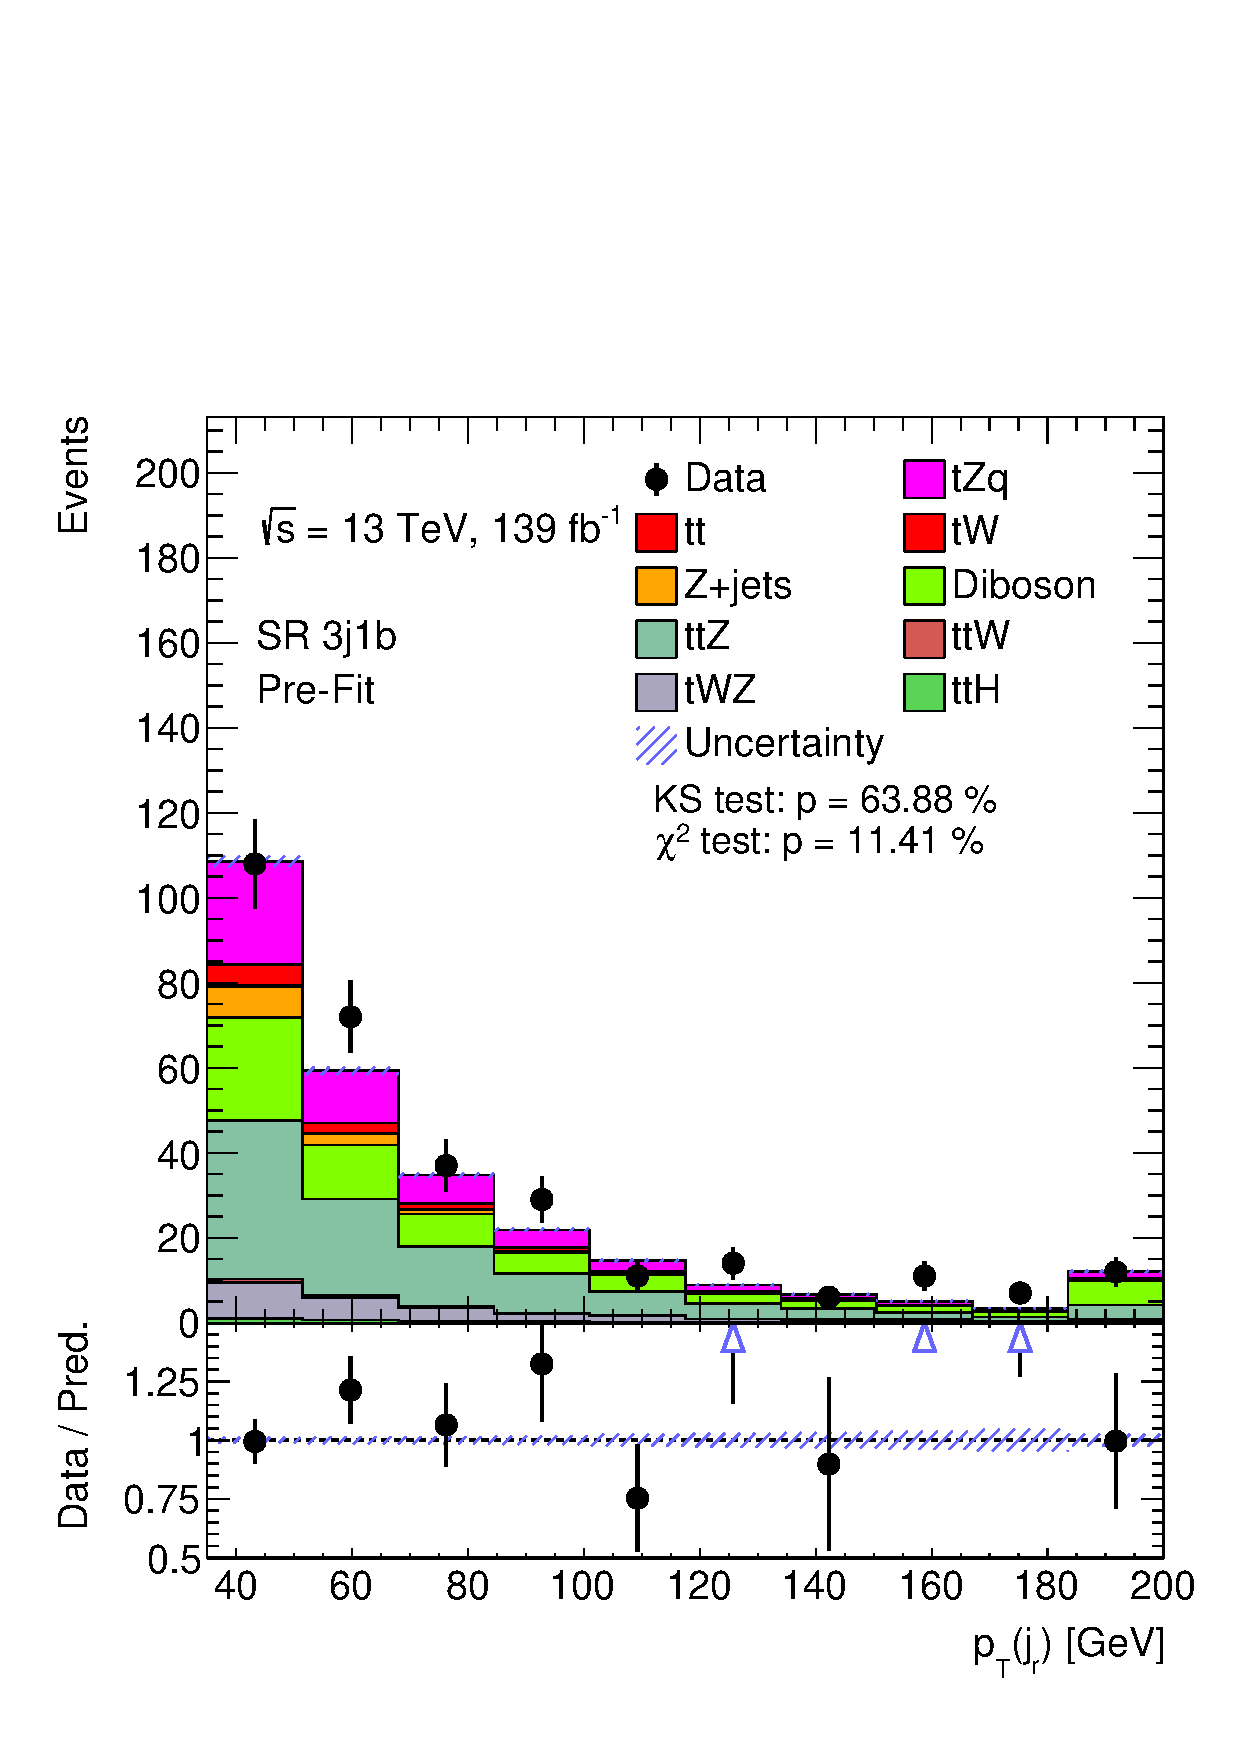
\includegraphics[width=\linewidth]{ubonn-thesis/Chapters/Chapters_06/Figure/Input_distribution/SR_3j1b_ptjf.pdf} 
  \end{subfigure} 
  \newline
  \vspace*{0.4cm}
  \begin{subfigure}[b]{0.33\linewidth}
    \centering
    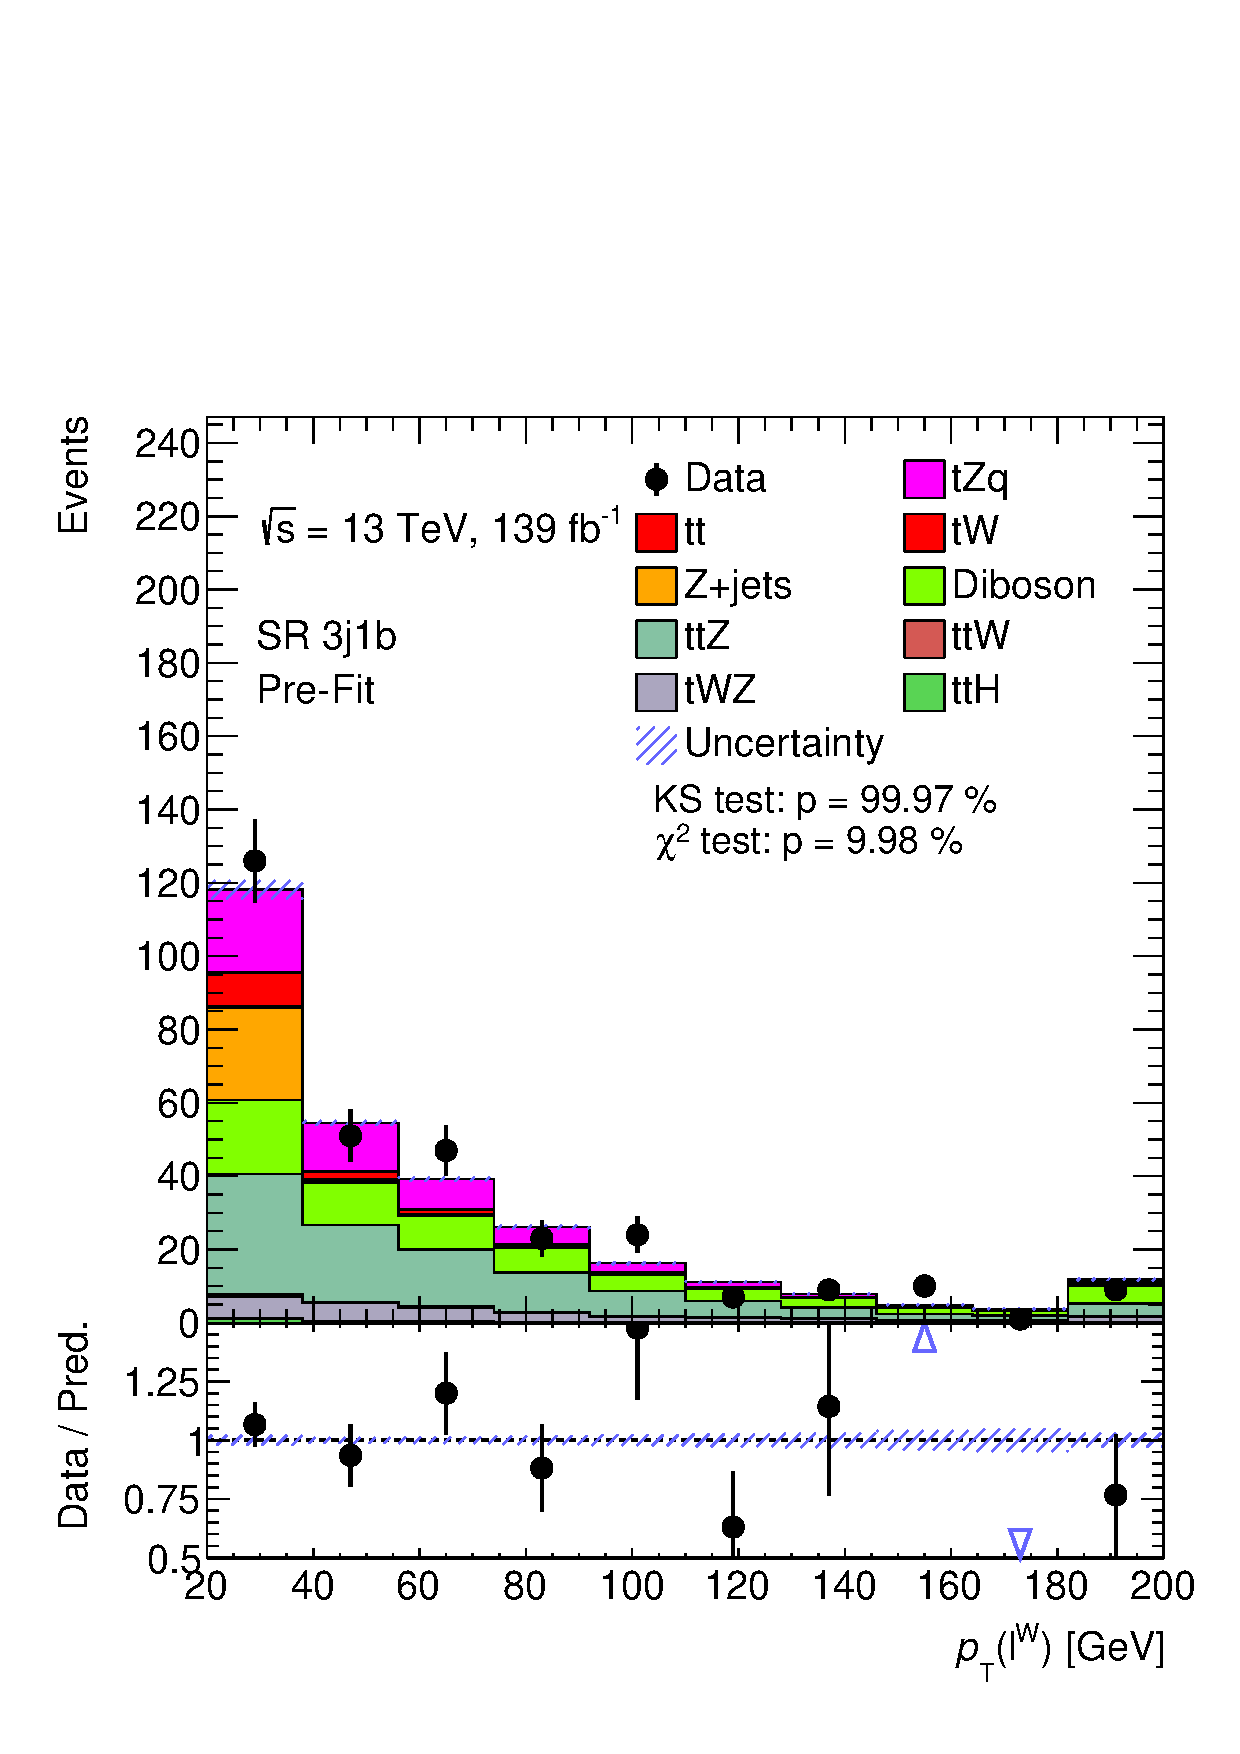
\includegraphics[width=\linewidth]{ubonn-thesis/Chapters/Chapters_06/Figure/Input_distribution/SR_3j1b_lepW_pt.pdf} 
  \end{subfigure}%%
  \begin{subfigure}[b]{0.33\linewidth}
    \centering
    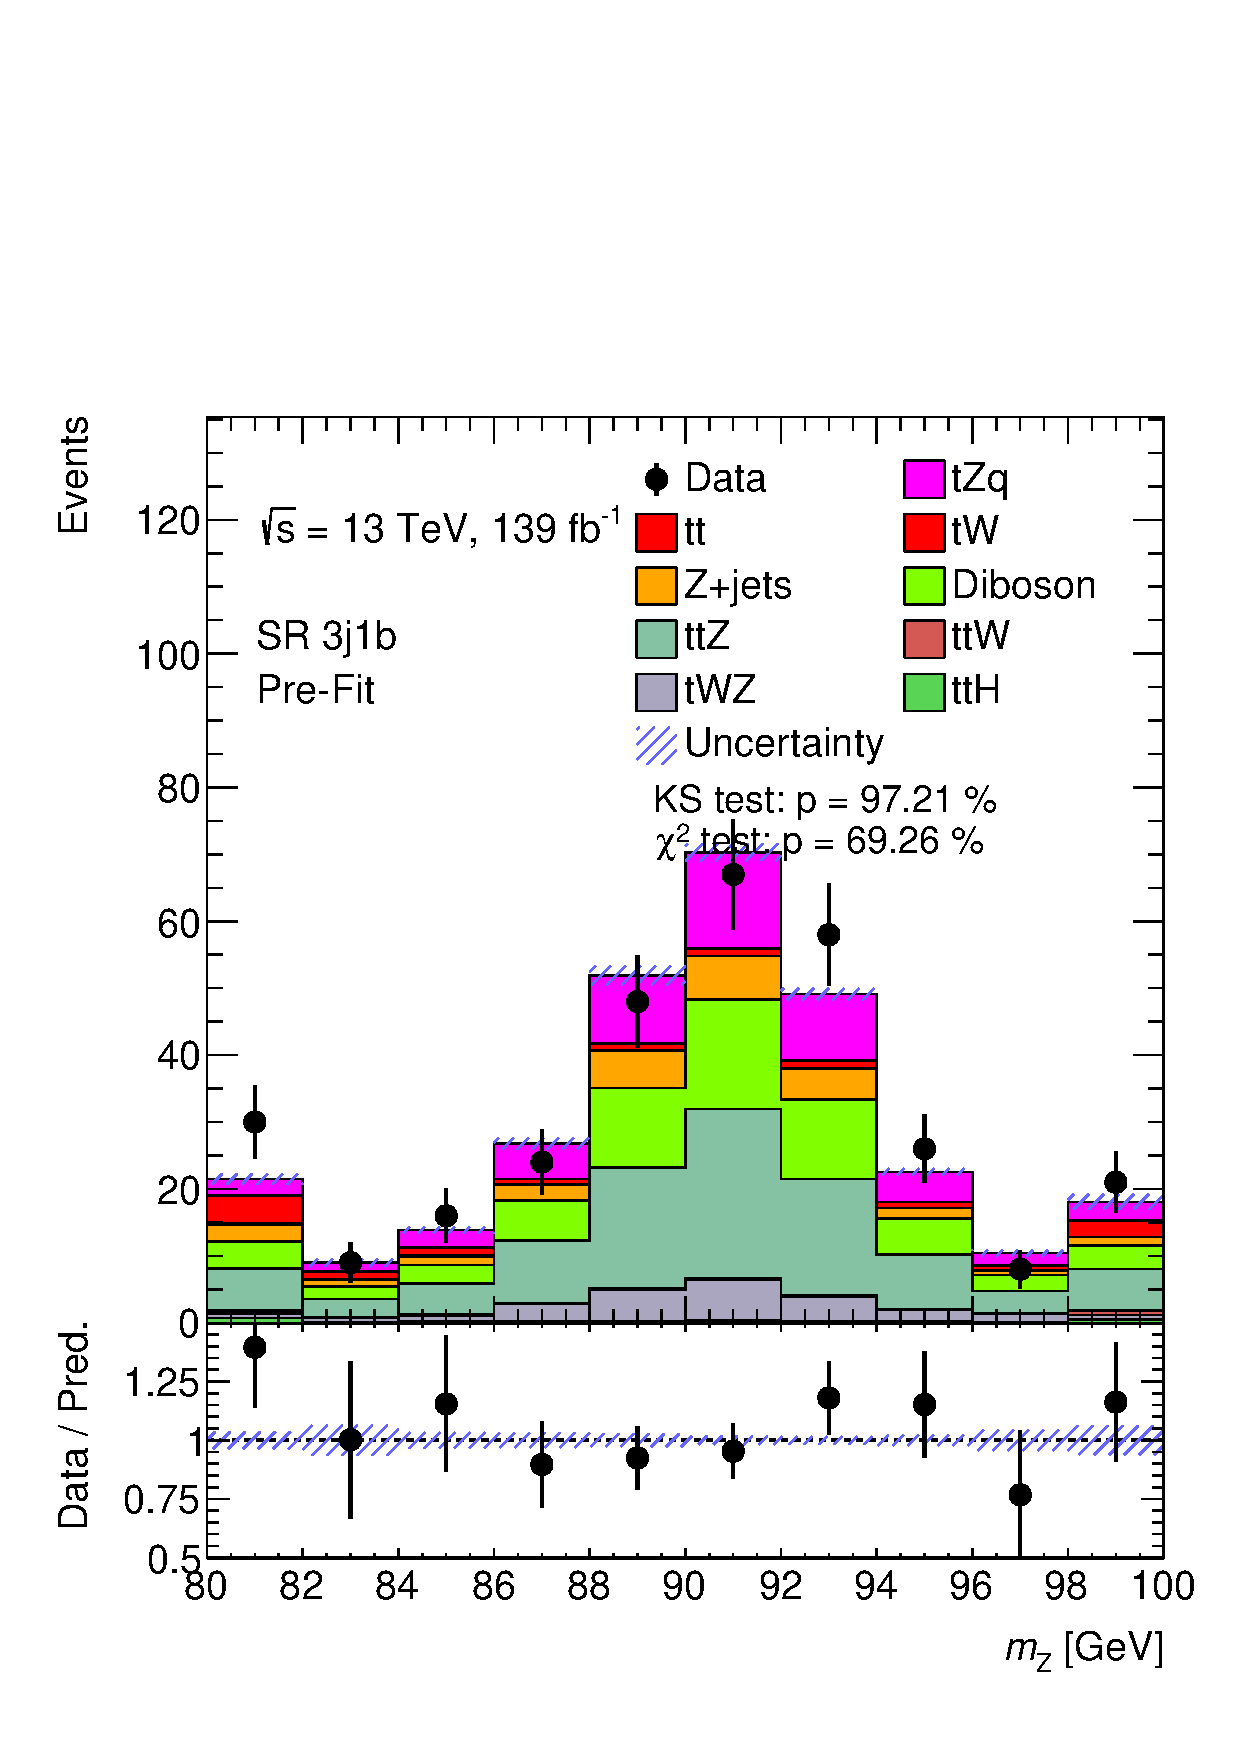
\includegraphics[width=\linewidth]{ubonn-thesis/Chapters/Chapters_06/Figure/Input_distribution/SR_3j1b_MZ.pdf} 
  \end{subfigure}
  \begin{subfigure}[b]{0.33\linewidth}
    \centering
    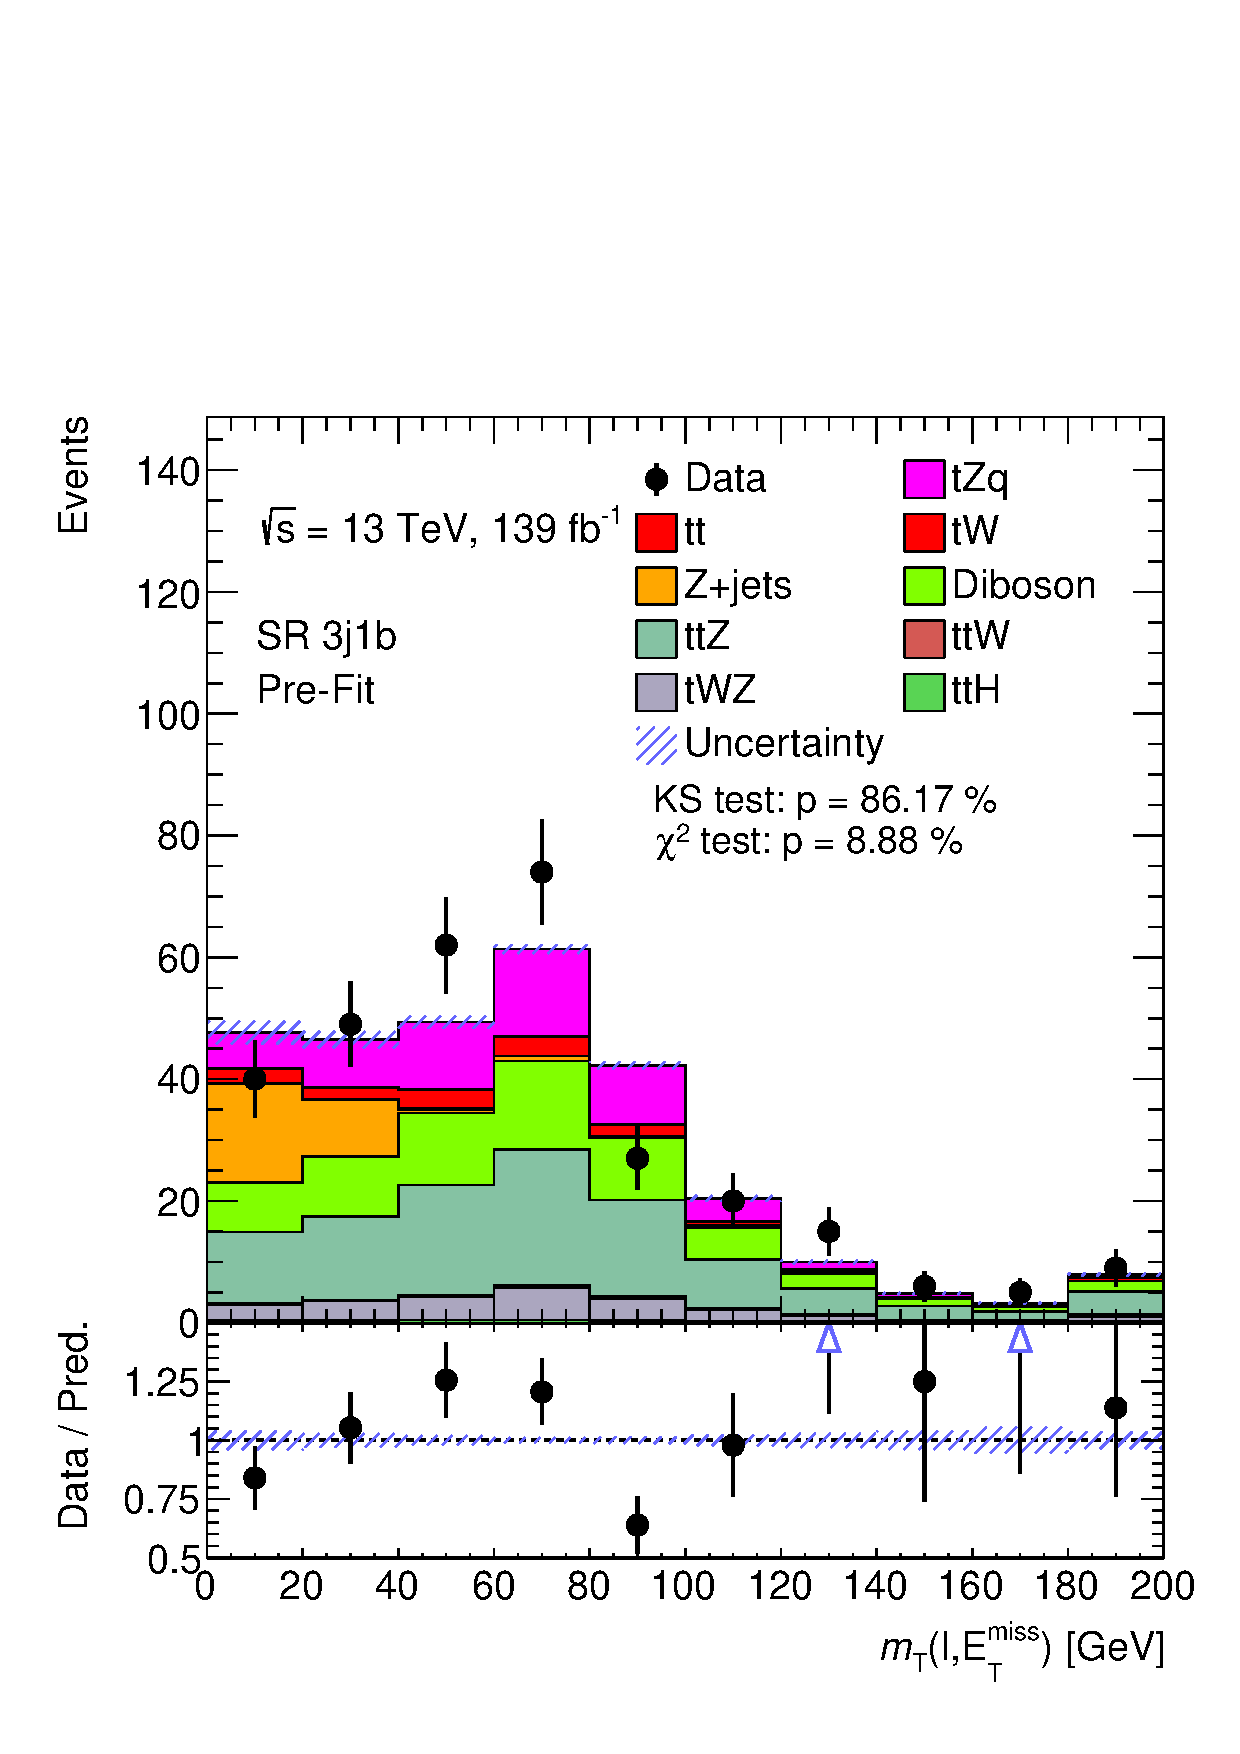
\includegraphics[width=\linewidth]{ubonn-thesis/Chapters/Chapters_06/Figure/Input_distribution/SR_3j1b_mtW.pdf} 
  \end{subfigure} 
  \newline
  \vspace*{0.4cm}
  \begin{subfigure}[b]{0.33\linewidth}
    \centering
    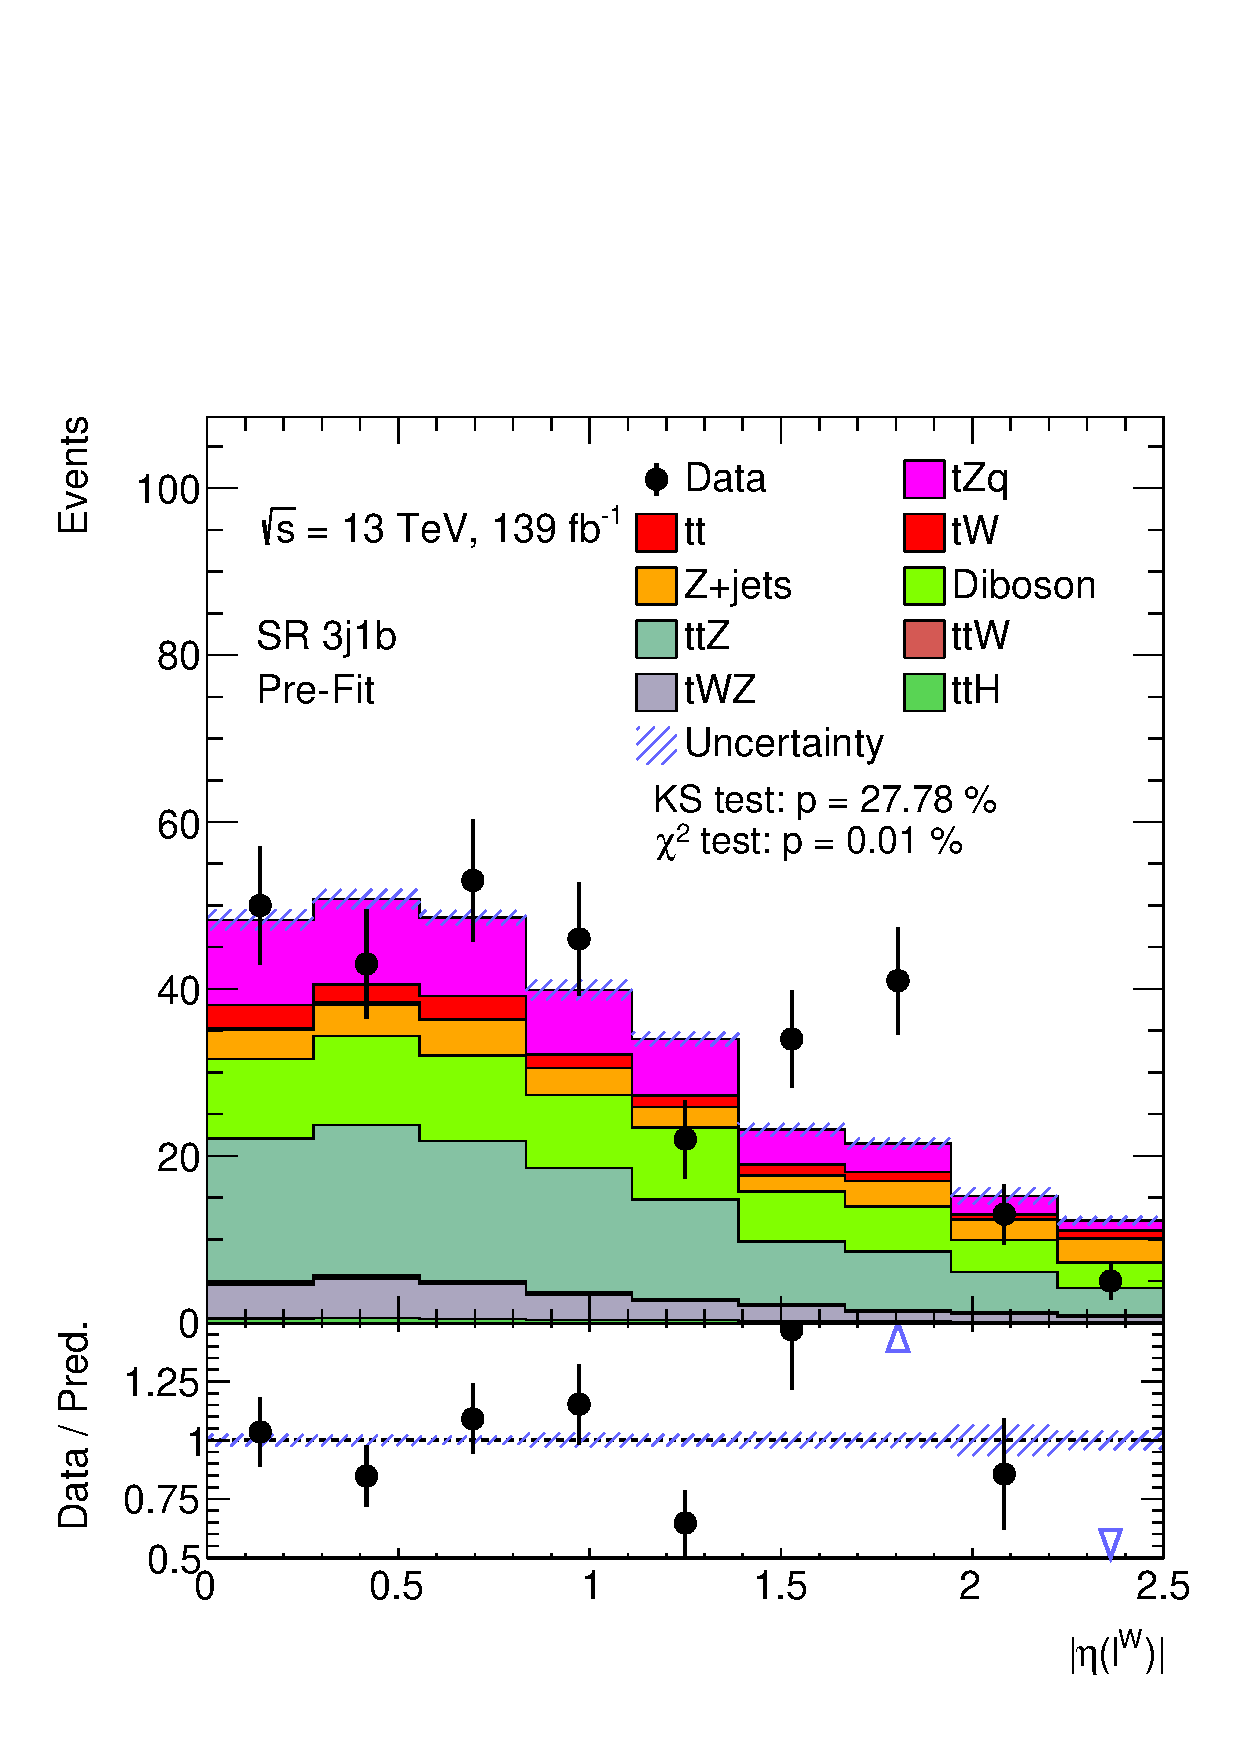
\includegraphics[width=\linewidth]{ubonn-thesis/Chapters/Chapters_06/Figure/Input_distribution/SR_3j1b_lepW_eta.pdf} 
  \end{subfigure}%%
  \begin{subfigure}[b]{0.33\linewidth}
    \centering
    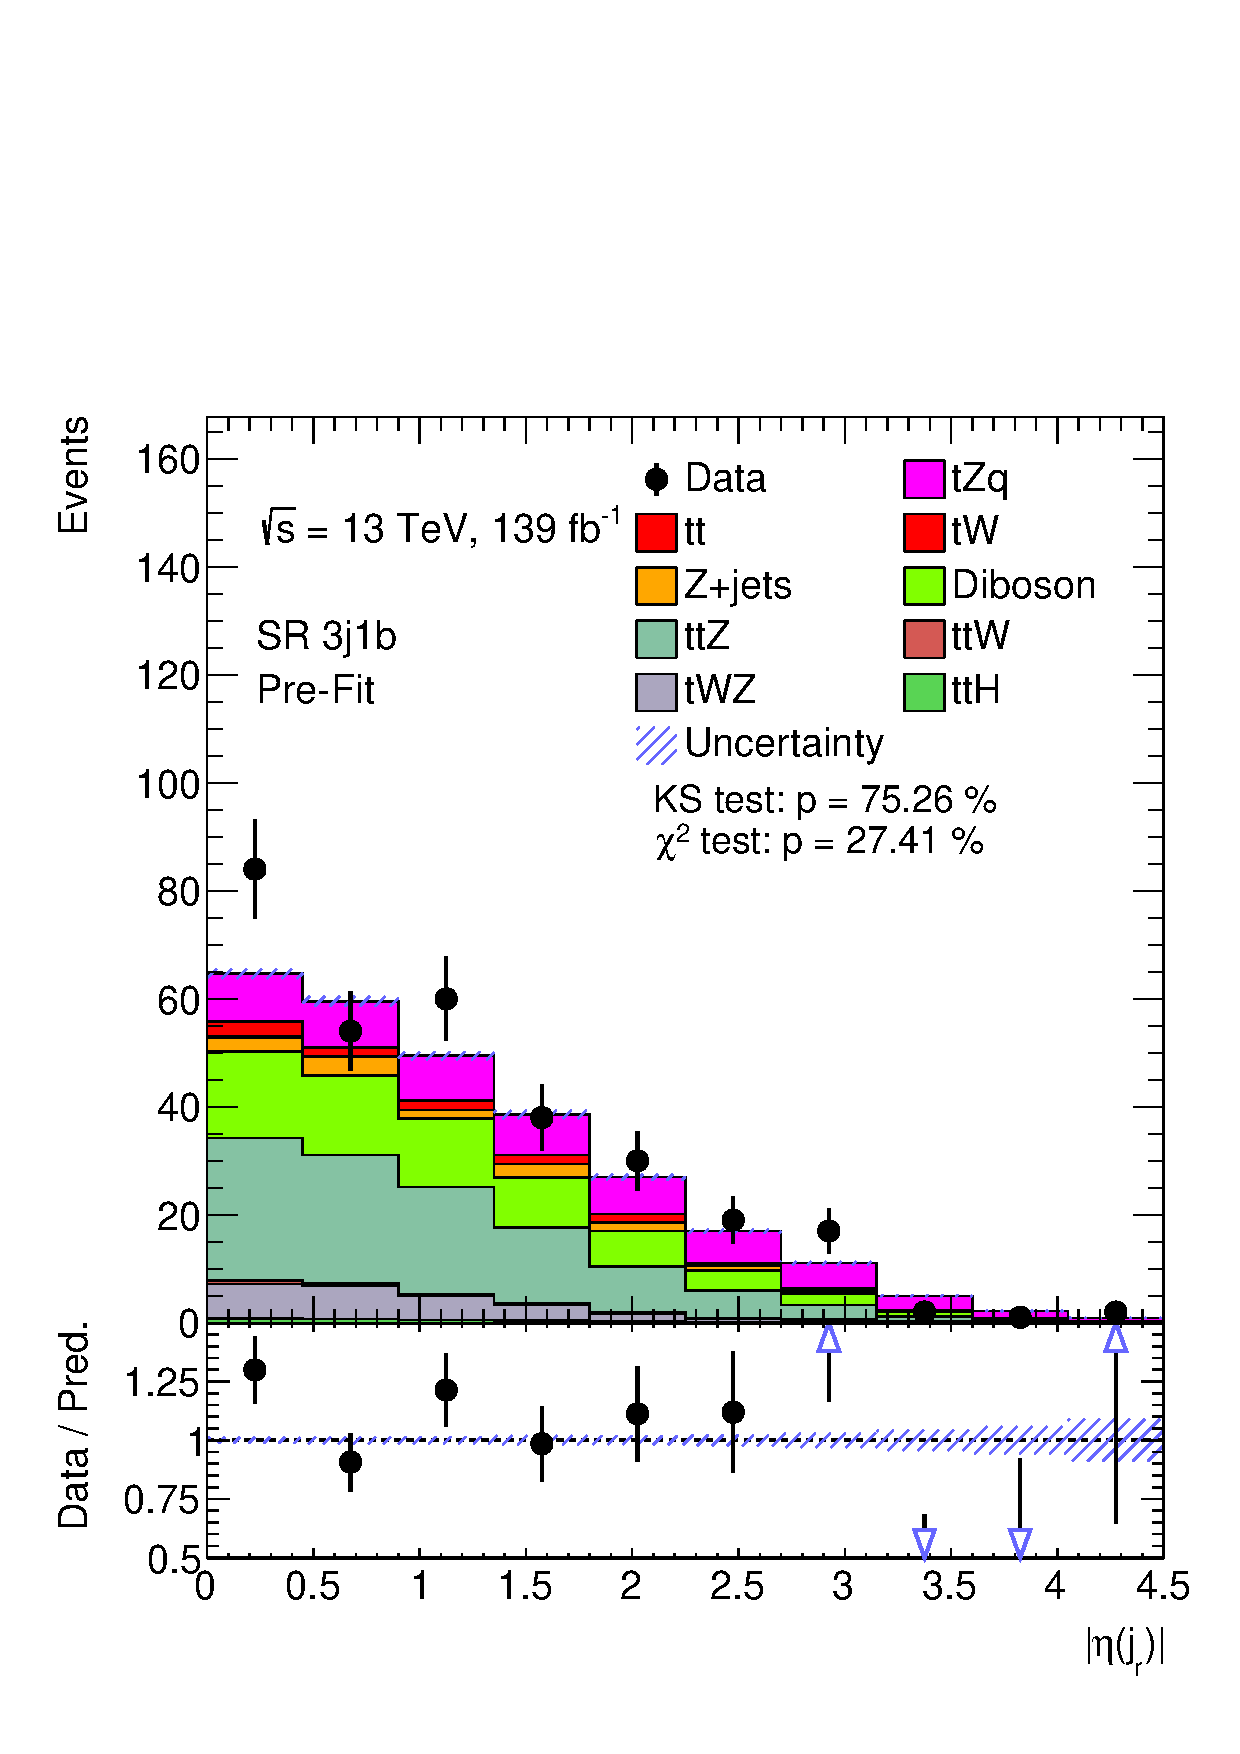
\includegraphics[width=\linewidth]{ubonn-thesis/Chapters/Chapters_06/Figure/Input_distribution/SR_3j1b_etajf.pdf} 
  \end{subfigure}
  \begin{subfigure}[b]{0.33\linewidth}
    \centering
    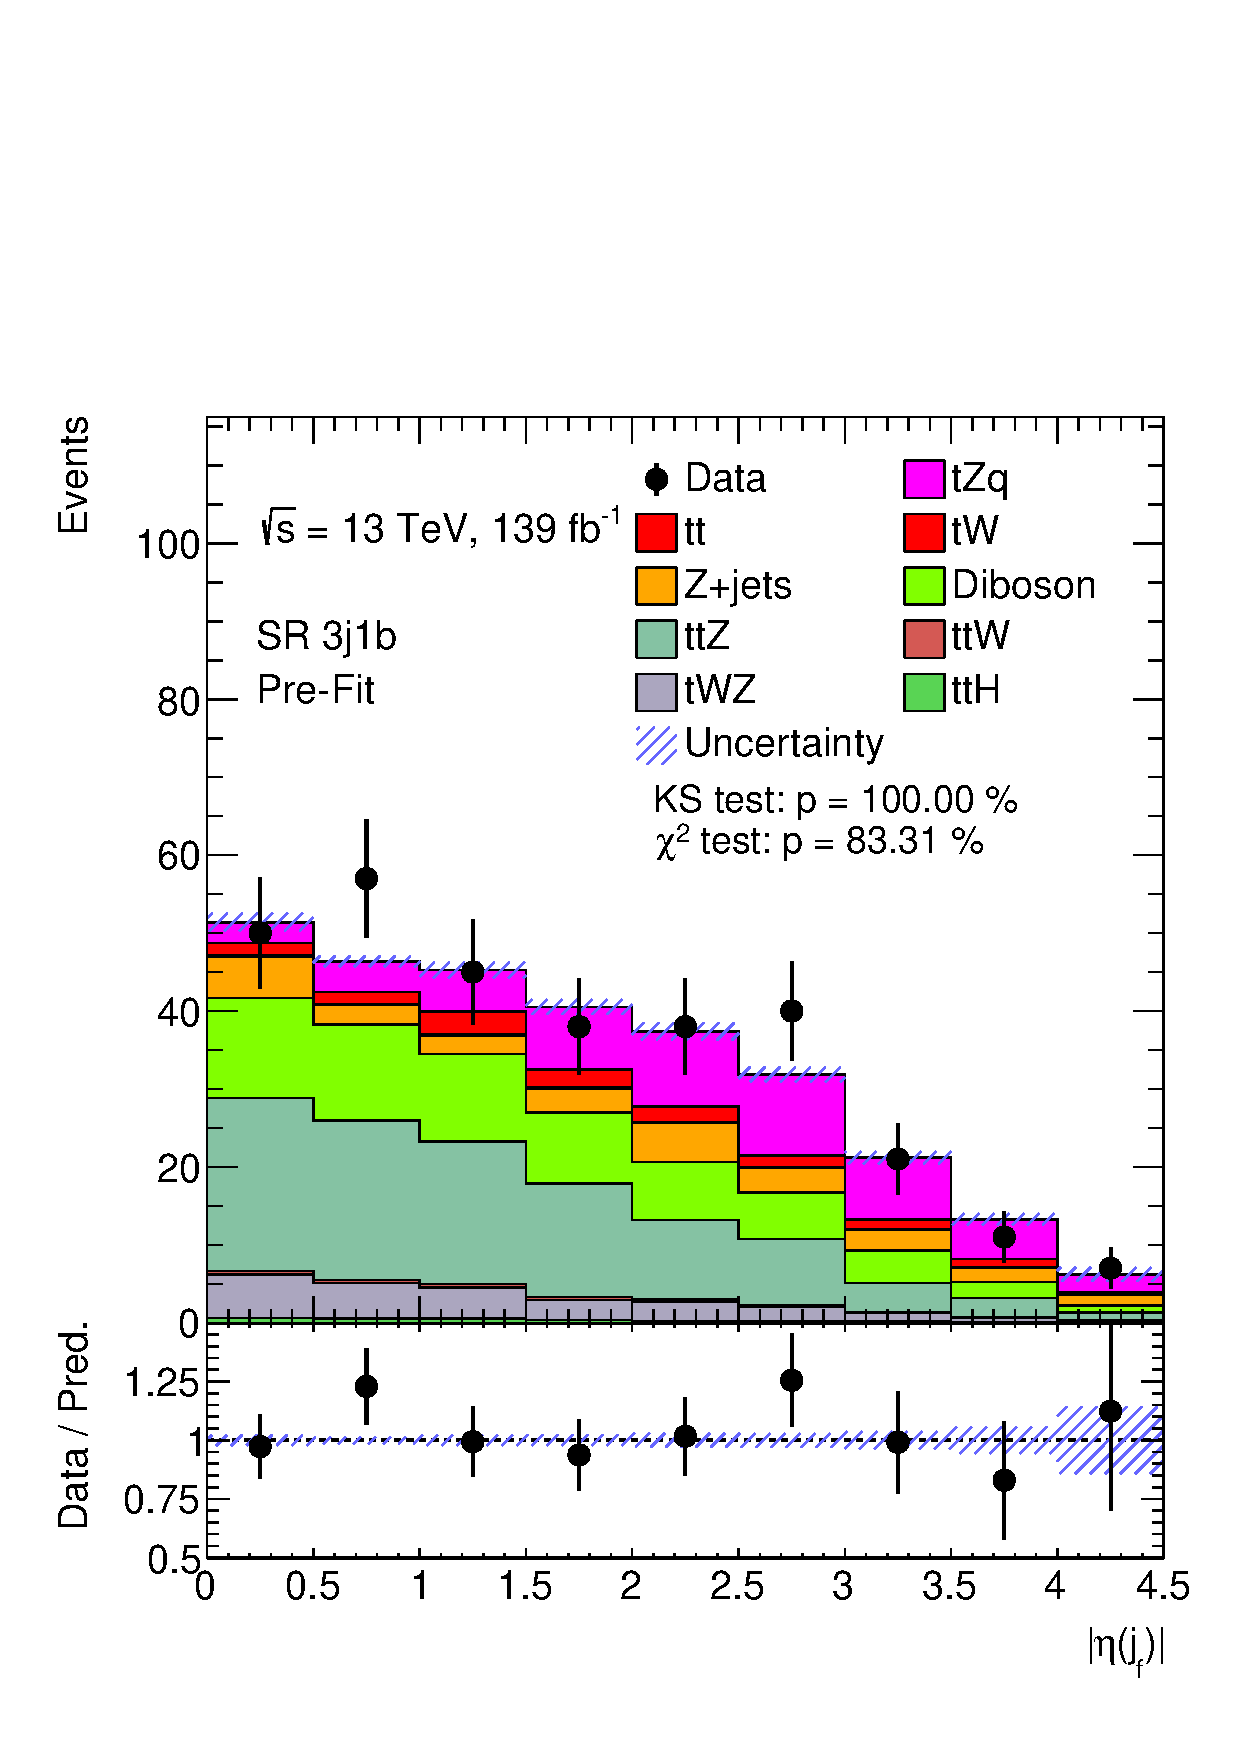
\includegraphics[width=\linewidth]{ubonn-thesis/Chapters/Chapters_06/Figure/Input_distribution/SR_3j1b_forwardjet_eta.pdf} 
  \end{subfigure} 
   \caption{Stacked kinematic plots of neural-network training variables of the SR 3j1b, in order of significance. Both signal and backgrounds are normalised to the expected number of events before the fit. The uncertainty band includes statistical uncertainties for signal and backgrounds}
  \label{fig_signal4} 
\end{figure}


\begin{figure}[!h] 
  \begin{subfigure}[b]{0.33\linewidth}
    \centering
    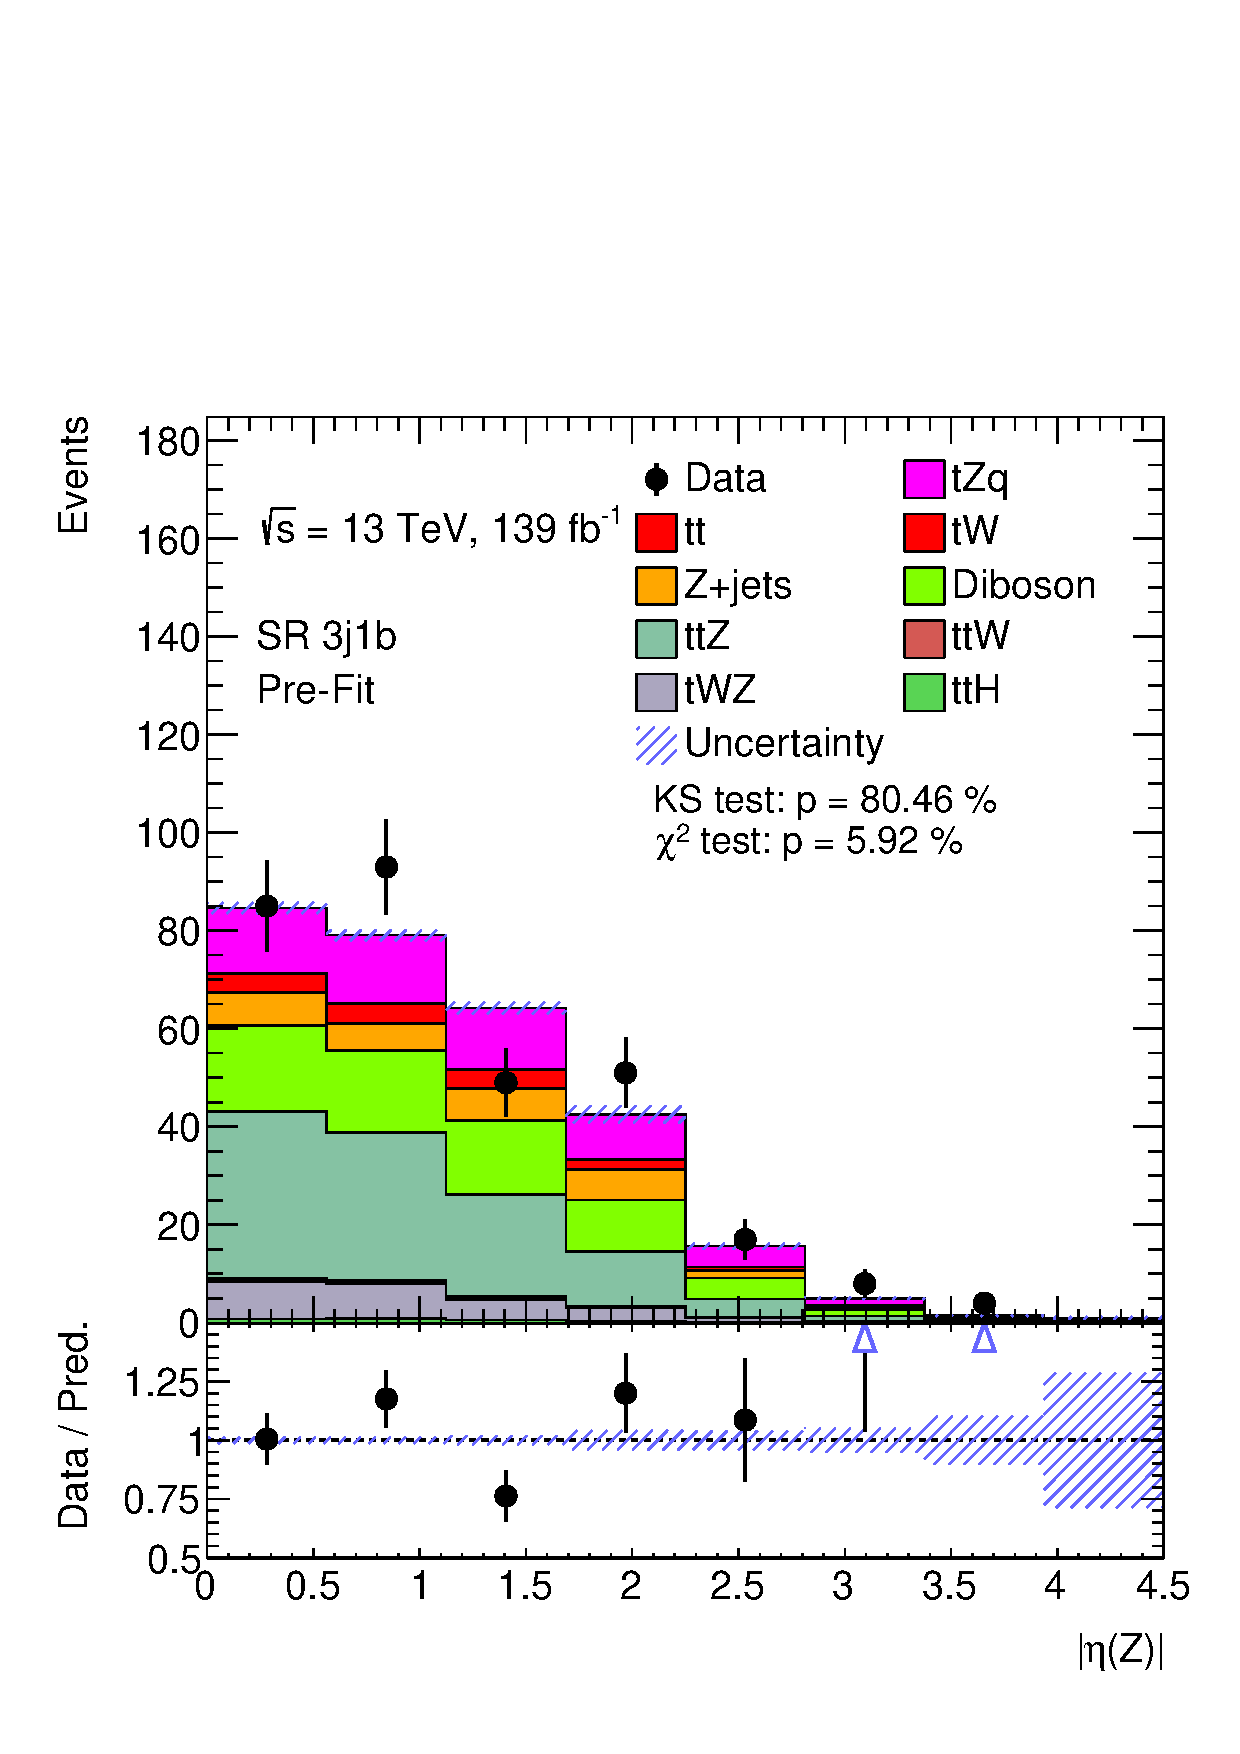
\includegraphics[width=\linewidth]{ubonn-thesis/Chapters/Chapters_06/Figure/Input_distribution/SR_3j1b_Z_eta.pdf} 
  \end{subfigure} 
  \begin{subfigure}[b]{0.33\linewidth}
    \centering
    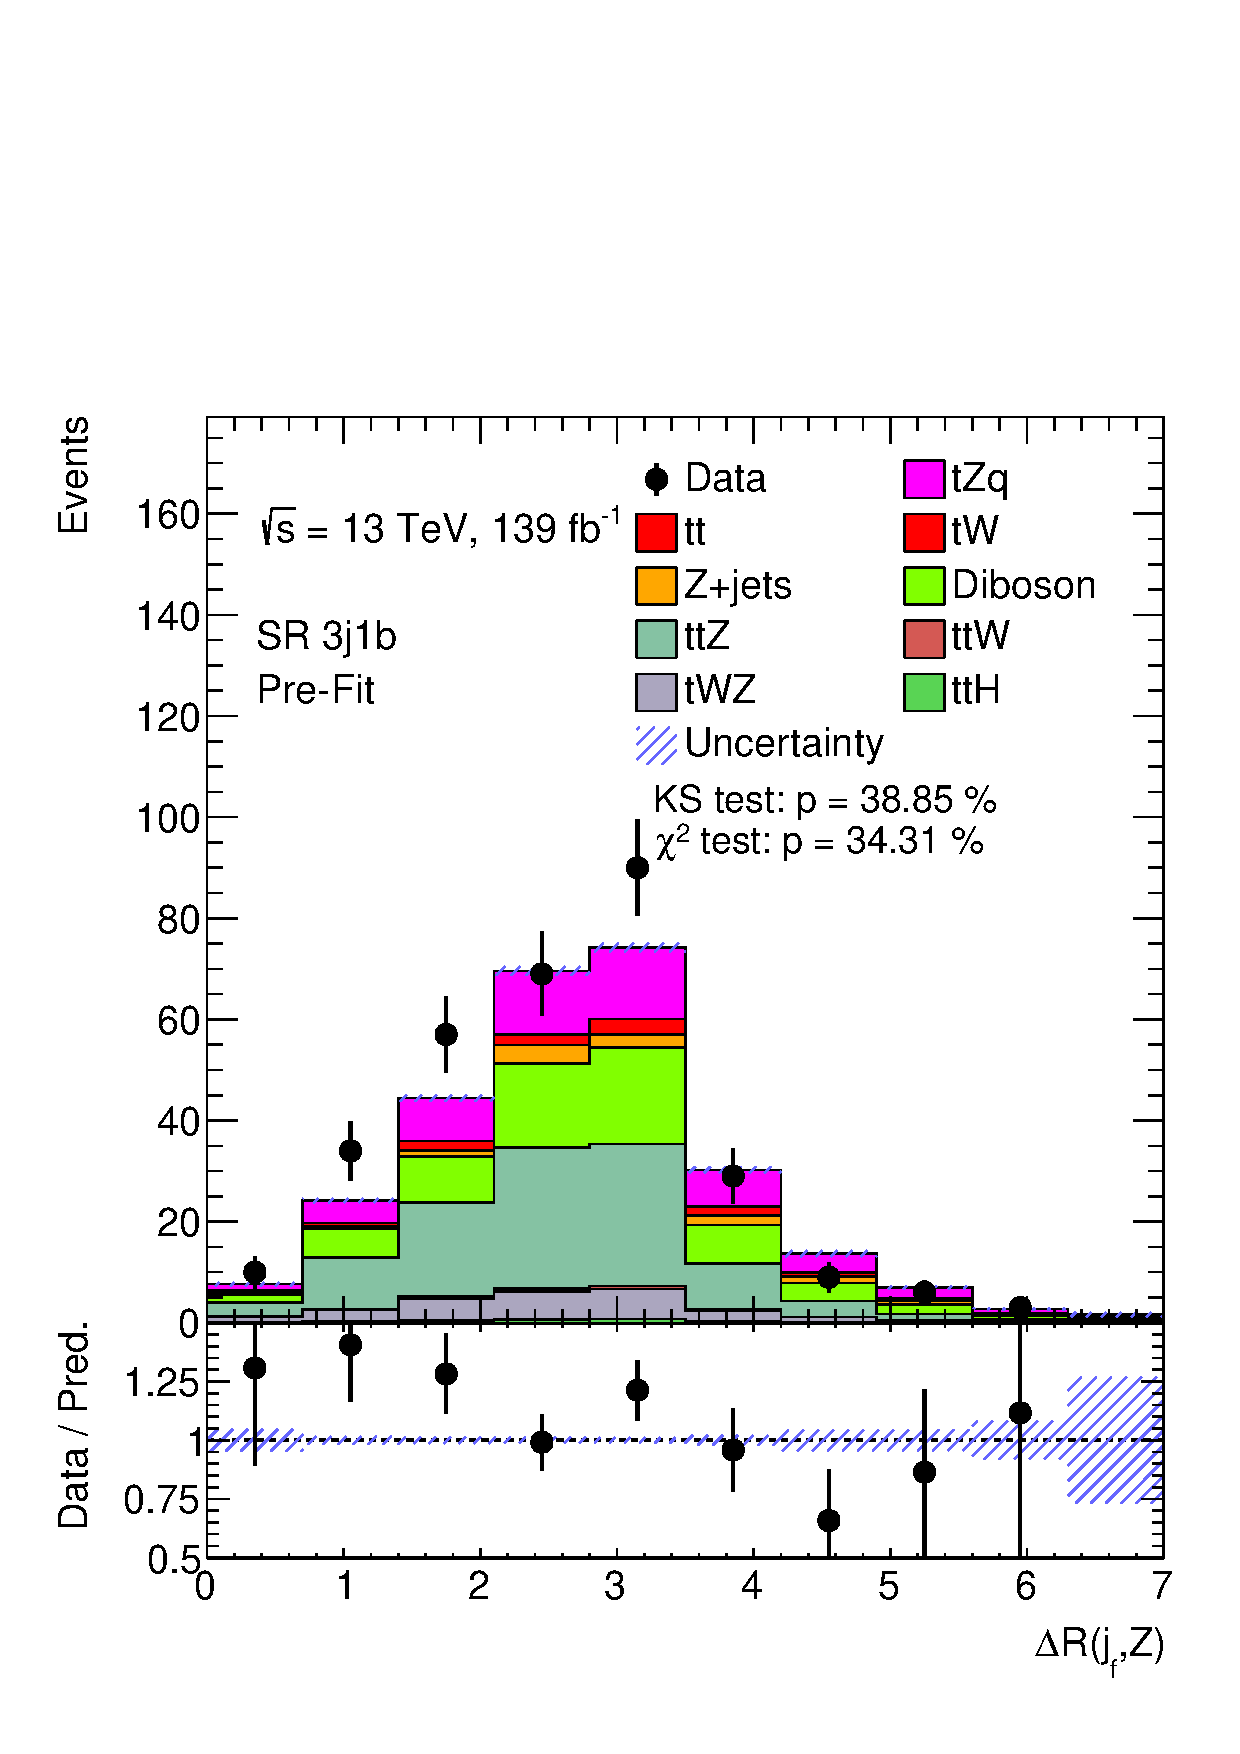
\includegraphics[width=\linewidth]{ubonn-thesis/Chapters/Chapters_06/Figure/Input_distribution/SR_3j1b_dRjfZ.pdf} 
  \end{subfigure}%% 
  \begin{subfigure}[b]{0.33\linewidth}
    \centering
    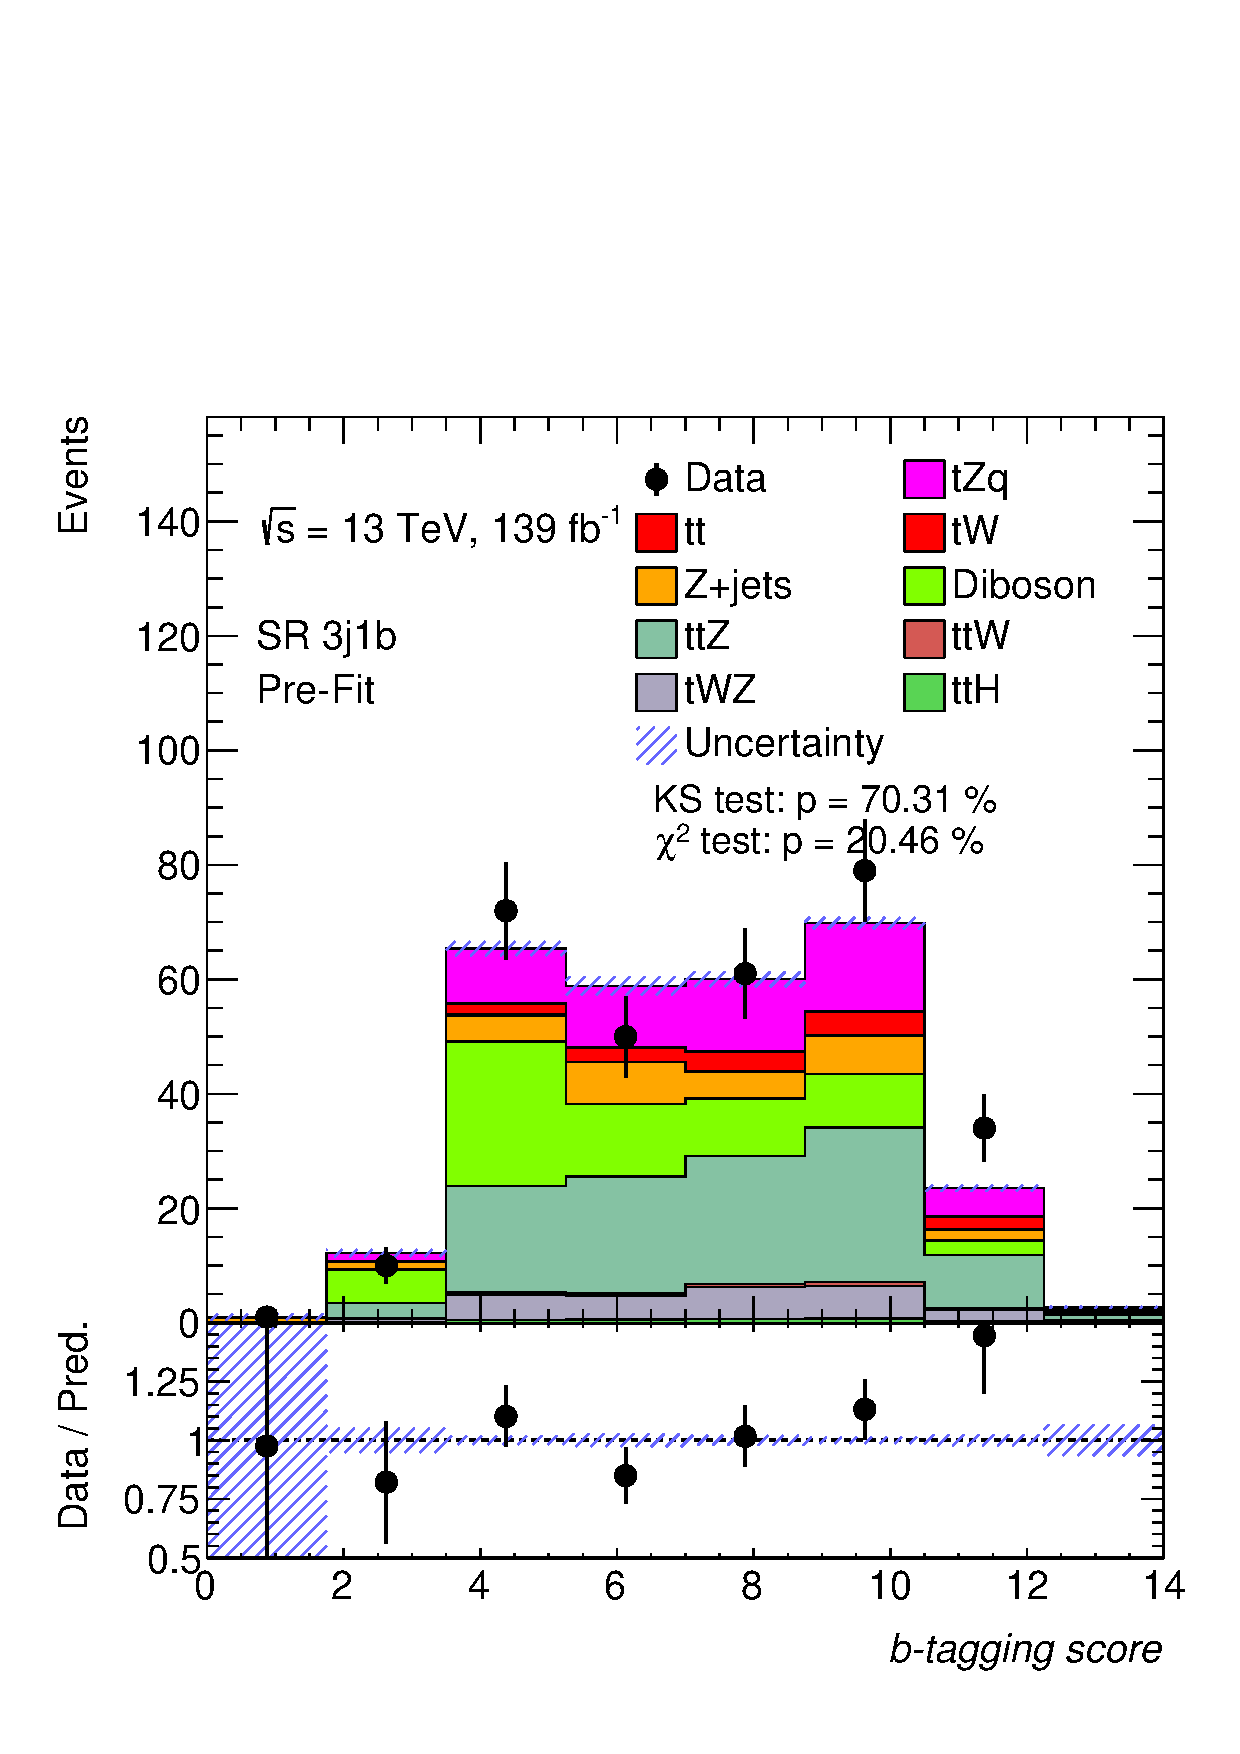
\includegraphics[width=\linewidth]{ubonn-thesis/Chapters/Chapters_06/Figure/Input_distribution/SR_3j1b_btag.pdf} 
  \end{subfigure}
  \centering
  \begin{subfigure}[b]{0.33\linewidth}
    \centering
    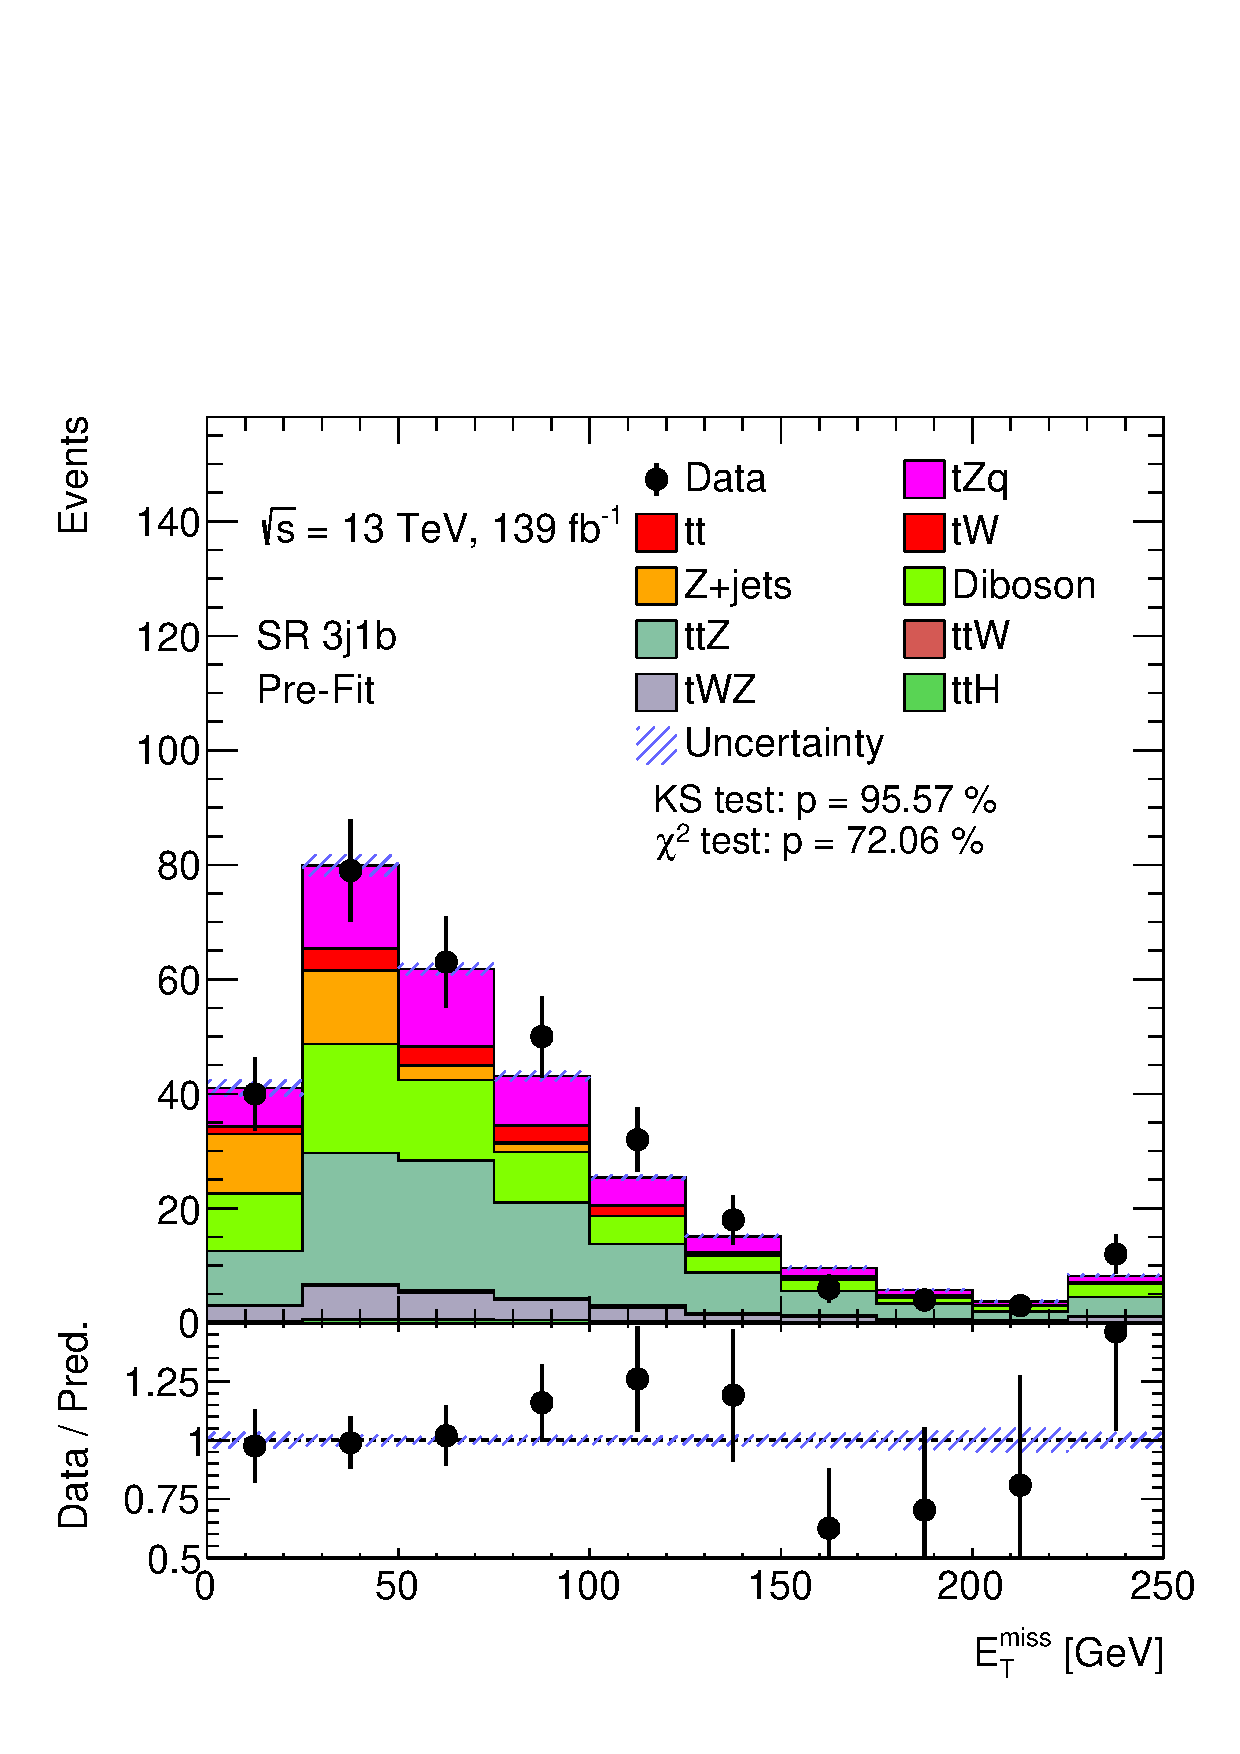
\includegraphics[width=\linewidth]{ubonn-thesis/Chapters/Chapters_06/Figure/Input_distribution/SR_3j1b_MissEt.pdf} 
  \end{subfigure}
  \caption{Stacked kinematic plots of neural-network training variables of the SR 3j1b, in order of significance. Both signal and backgrounds are normalised to the expected number of events before the fit. The uncertainty band includes statistical uncertainties for signal and backgrounds}
  \label{fig_signal5}
  \end{figure}



\subsection{NN training in the SRs and $t\Bar{t}Z$ CRs}

In this section, the results of the NN training is presented. Before the training the MC samples are divided into training and test samples which is also called validation samples. The main idea of splitting the dataset into a training and a validation set is to prevent the model from over-fitting. Training dataset is the set of data that is used to train and make the model learn the hidden features/patterns in the data. In each epoch, the same training data is fed to the neural network repeatedly, and the model continues to learn the features of the data. The validation dataset is the set of data separate from the training set, that is used to validate our model performance during training. The validation process gives information that helps us tune the model's hyperparameters and configurations accordingly.

%% SR 2j1b

\begin{figure}[!h] 
  \begin{subfigure}[b]{0.48\linewidth}
    \centering
    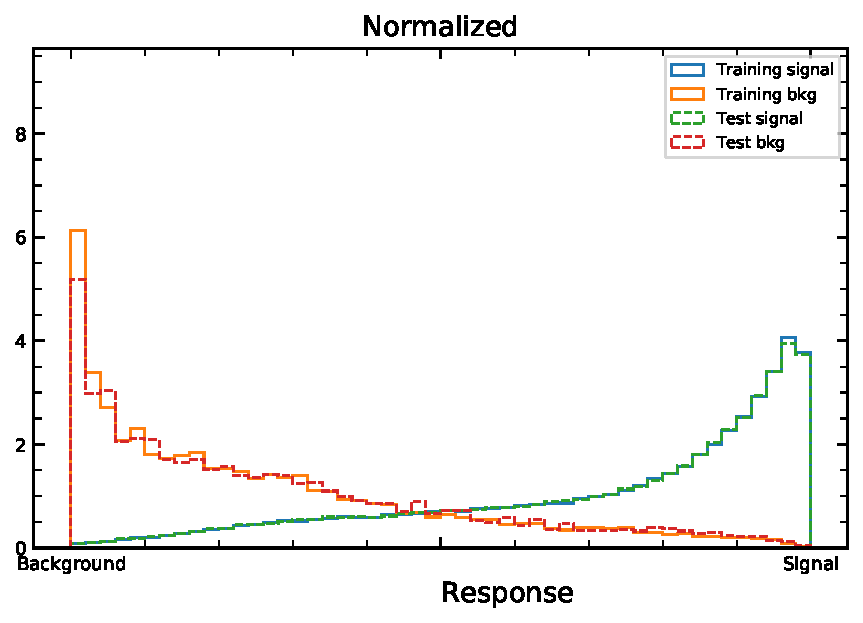
\includegraphics[width=0.95\linewidth]{ubonn-thesis/Chapters/Chapters_06/Figure/SR_2j1b/NormalizedResponse_PLV_2j1b_L27_20_10_06Oct2021.pdf} 
    \caption{} 
    \label{SR:2j1b:NNout} 
  \end{subfigure}%% 
  \vspace*{0.4cm}
  \begin{subfigure}[b]{0.48\linewidth}
    \centering
    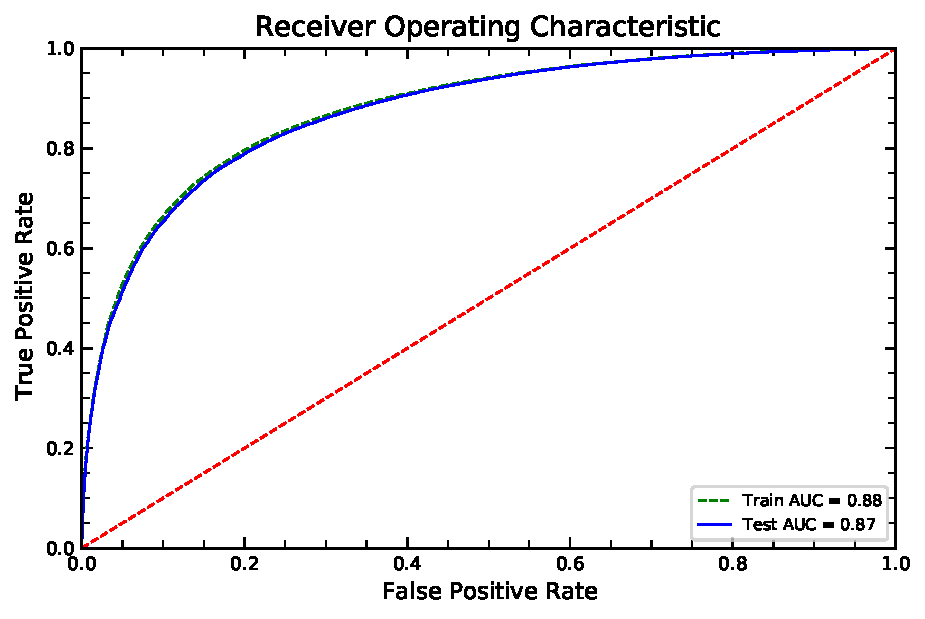
\includegraphics[width=\linewidth]{ubonn-thesis/Chapters/Chapters_06/Figure/SR_2j1b/ROC_PLV_2j1b_L27_20_10_06Oct2021.pdf} 
    % \vspace*{-0.4cm}
    \caption{} 
    \label{SR:2j1b:ROC} 
  \end{subfigure} 
  \vspace*{0.4cm}
  \begin{subfigure}[b]{0.48\linewidth}
    \centering
    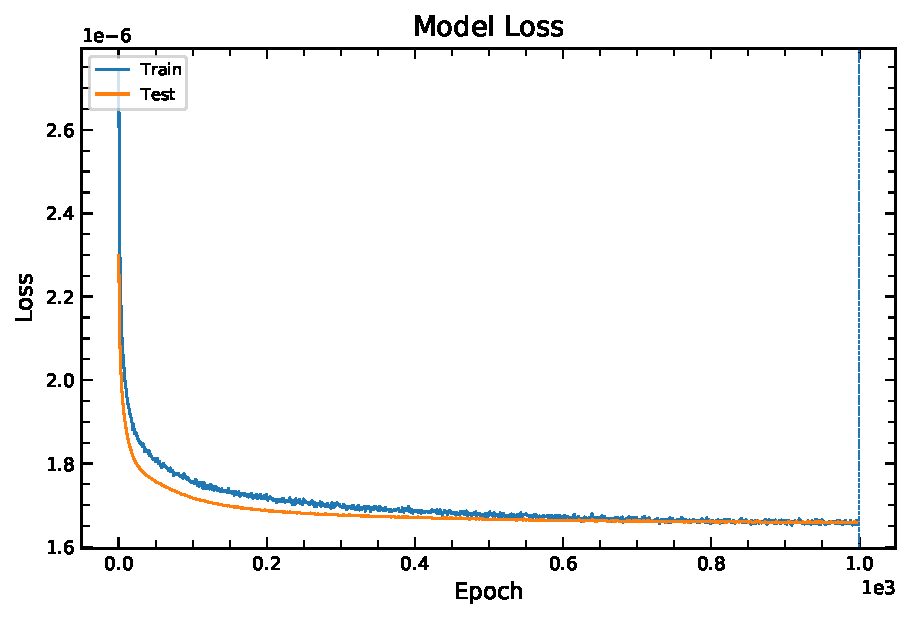
\includegraphics[width=\linewidth]{ubonn-thesis/Chapters/Chapters_06/Figure/SR_2j1b/loss_PLV_2j1b_L27_20_10_06Oct2021.pdf} %\vspace*{-0.4cm}
    \caption{} 
    \label{SR:2j1b:loss} 
  \end{subfigure}%%
  \begin{subfigure}[b]{0.48\linewidth}
    \centering
    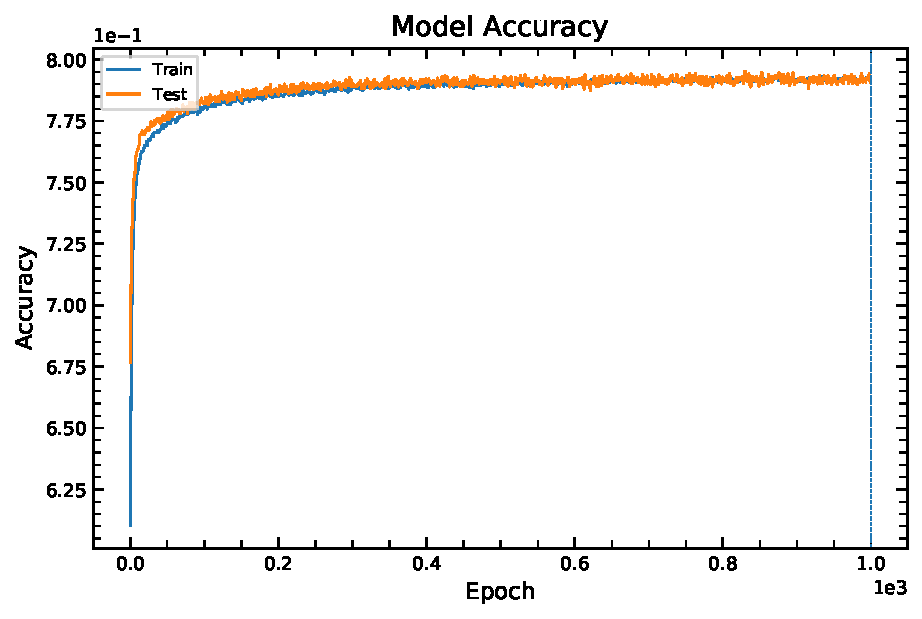
\includegraphics[width=\linewidth]{ubonn-thesis/Chapters/Chapters_06/Figure/SR_2j1b/acc_PLV_2j1b_L27_20_10_06Oct2021.pdf} 
    % \vspace*{-0.4cm}
    \caption{} 
    \label{SR:2j1b:acc} 
  \end{subfigure}
  \vspace*{-0.5cm}
  \caption{Neural Network training output in the SR 2j1b. (a) shows the normalized response of the NN, (b) shows the ROC curve , (c) shows the loss variation during the training and (d) shows the model accuracy for both training and test samples}
  \label{SR:2j1b:NN} 
\end{figure}

% SR 3j1b (a)

%\vspace*{-0.8cm}
\begin{figure}[h!]
    \begin{subfigure}[b]{0.48\linewidth}
    \centering
    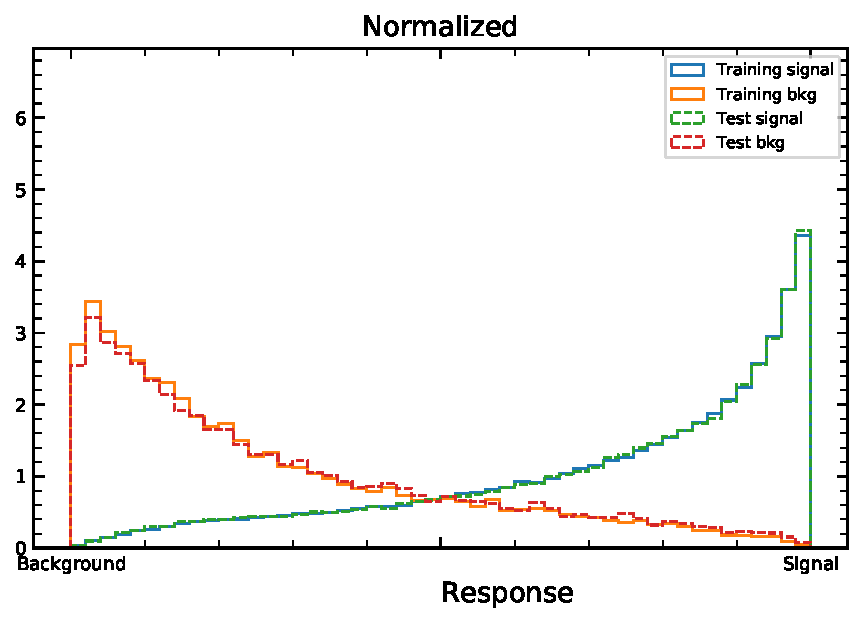
\includegraphics[width=0.95\linewidth]{ubonn-thesis/Chapters/Chapters_06/Figure/SR_3j1b/NormalizedResponse_PLV_3j1b_L27_20_10_06Oct2021.pdf} 
    \caption{} 
    \label{SR:3j1b:NNout} 
  \end{subfigure}%% 
  \vspace*{0.4cm}
  \begin{subfigure}[b]{0.48\linewidth}
    \centering
    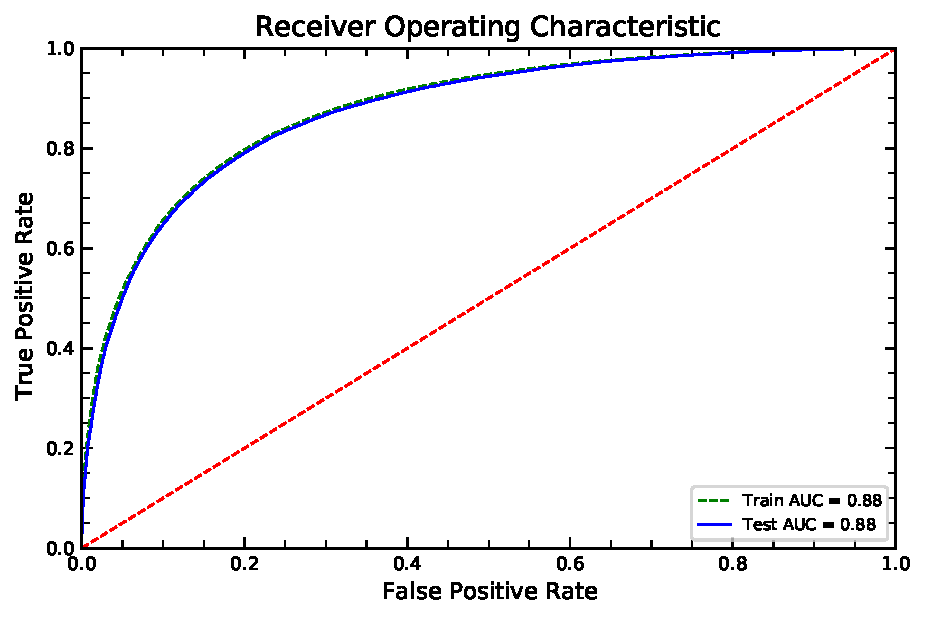
\includegraphics[width=\linewidth]{ubonn-thesis/Chapters/Chapters_06/Figure/SR_3j1b/ROC_PLV_3j1b_L27_20_10_06Oct2021.pdf} 
    % \vspace*{-0.4cm}
    \caption{} 
    \label{SR:3j1b:ROC} 
  \end{subfigure}
  \vspace*{-0.5cm}
  \caption{Neural Network training output in the SR 3j1b. (a) shows the normalized response of the NN, (b) shows the ROC curve for both training and test samples}
  \label{SR:3j1b:NN(a)}
\end{figure}

% SR 3j1b (b)

\begin{figure}[!h] 
  \vspace*{-0.3cm}
  \begin{subfigure}[b]{0.5\linewidth}
    \centering
    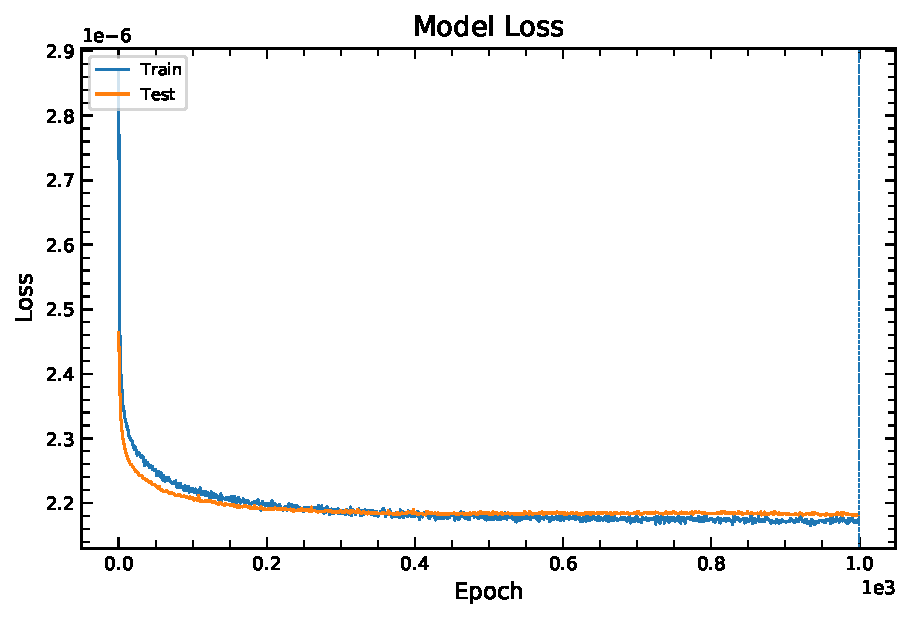
\includegraphics[width=\linewidth]{ubonn-thesis/Chapters/Chapters_06/Figure/SR_3j1b/loss_PLV_3j1b_L27_20_10_06Oct2021.pdf} %\vspace*{-0.4cm}
    \caption{} 
    \label{SR:3j1b:loss} 
  \end{subfigure}%%
  \begin{subfigure}[b]{0.5\linewidth}
    \centering
    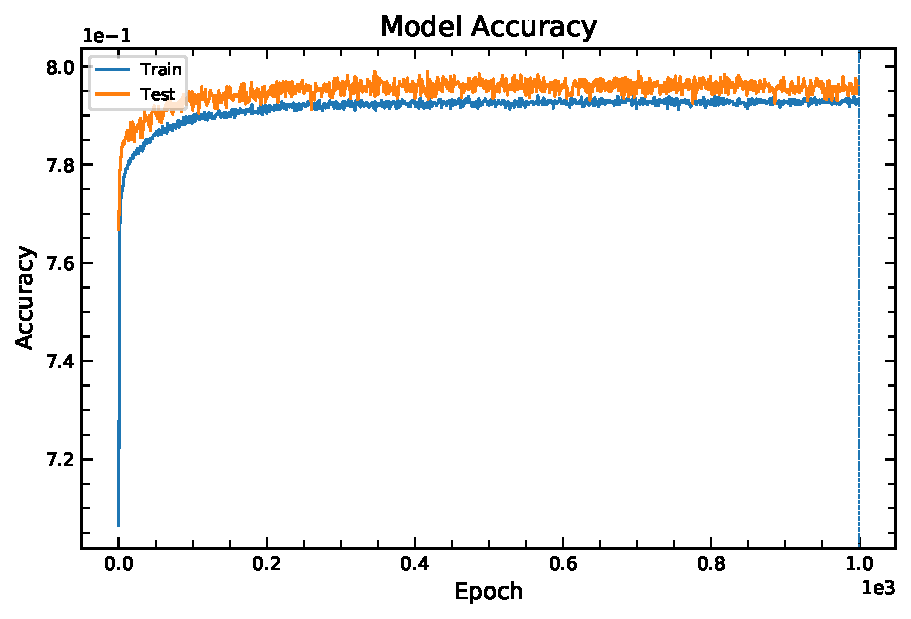
\includegraphics[width=\linewidth]{ubonn-thesis/Chapters/Chapters_06/Figure/SR_3j1b/acc_PLV_3j1b_L27_20_10_06Oct2021.pdf} 
    % \vspace*{-0.4cm}
    \caption{} 
    \label{SR:3j1b:acc} 
  \end{subfigure} 
  \vspace*{-0.5cm}
  \caption{Neural Network training output in the SR 3j1b. (a) shows the loss variation during the training and (b) shows the model accuracy for both training and test samples}
  \label{SR:3j1b:NN(b)} 
\end{figure}


%% CR 3j2b

\begin{figure}[!h] 
 % \vspace*{-0.2cm}
  \begin{subfigure}[b]{0.5\linewidth}
    \centering
    \vspace*{-0.2cm}
    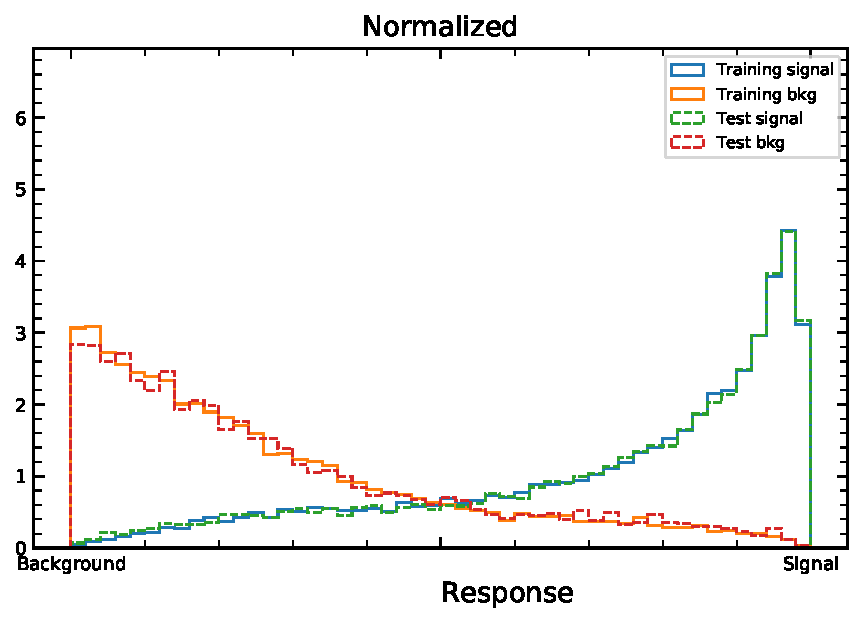
\includegraphics[width=0.95\linewidth]{ubonn-thesis/Chapters/Chapters_06/Figure/CR_3j2b/NormalizedResponse_PLV_3j2b_L27_20_10_06Oct2021.pdf} 
    \caption{} 
    \label{CR:3j2b:NNout} 
  \end{subfigure}%% 
  \vspace*{0.4cm}
  \begin{subfigure}[b]{0.5\linewidth}
    \centering
    \vspace*{-0.2cm}
    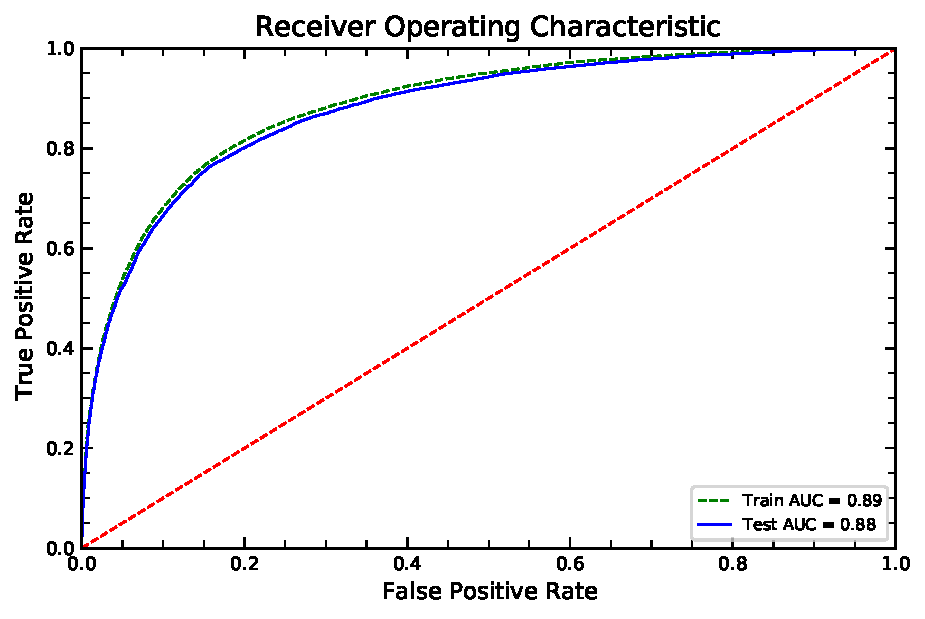
\includegraphics[width=\linewidth]{ubonn-thesis/Chapters/Chapters_06/Figure/CR_3j2b/ROC_PLV_3j2b_L27_20_10_06Oct2021.pdf} 
    % \vspace*{-0.4cm}
    \caption{} 
    \label{CR:3j2b:ROC} 
  \end{subfigure} 
  \vspace*{-0.4cm}
  \begin{subfigure}[b]{0.5\linewidth}
    \centering
    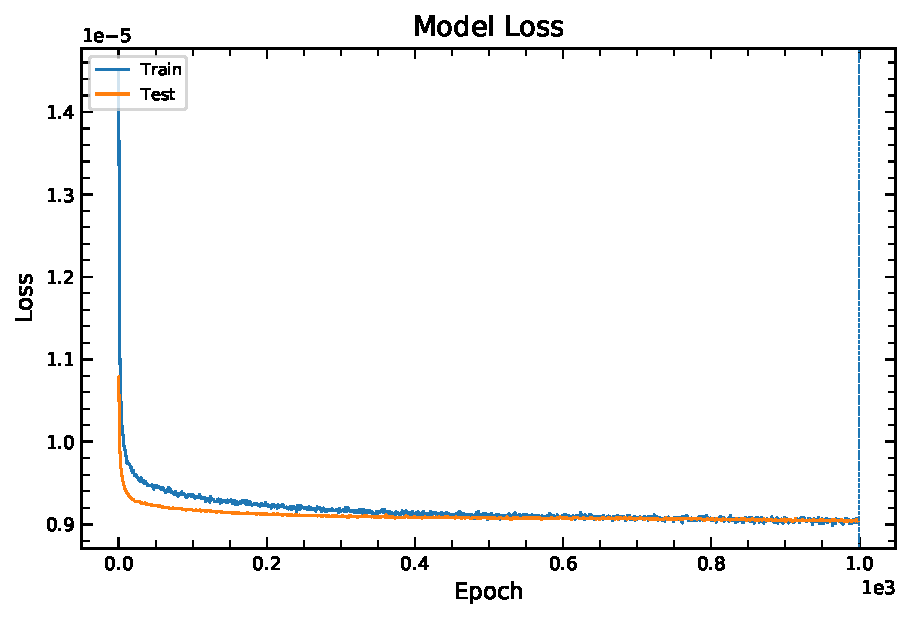
\includegraphics[width=\linewidth]{ubonn-thesis/Chapters/Chapters_06/Figure/CR_3j2b/loss_PLV_3j2b_L27_20_10_06Oct2021.pdf} %\vspace*{-0.4cm}
    \caption{} 
    \label{CR:3j2b:loss} 
  \end{subfigure}%%
  \begin{subfigure}[b]{0.5\linewidth}
    \centering
    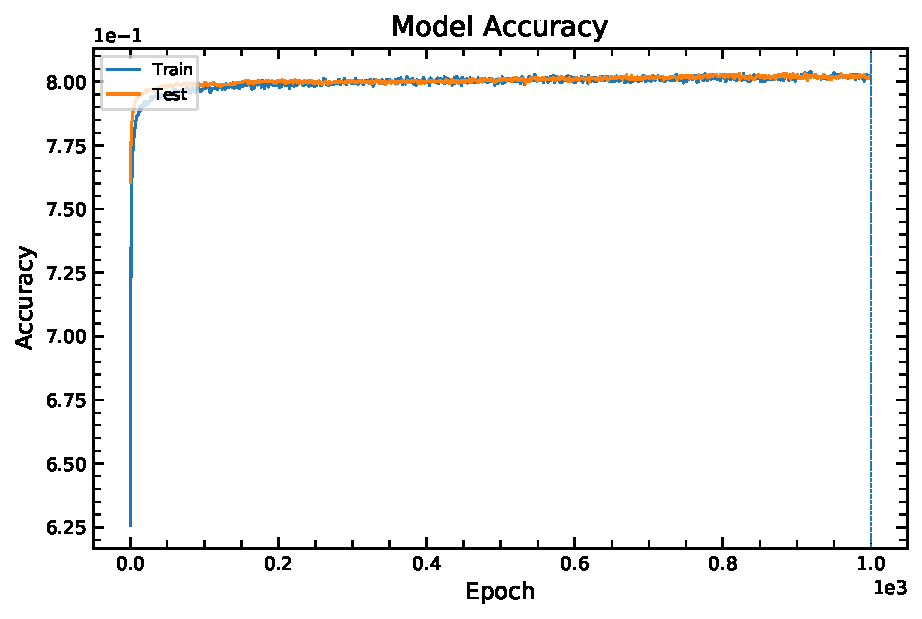
\includegraphics[width=\linewidth]{ubonn-thesis/Chapters/Chapters_06/Figure/CR_3j2b/acc_PLV_3j2b_L27_20_10_06Oct2021.pdf} 
    % \vspace*{-0.4cm}
    \caption{} 
    \label{CR:3j2b:acc} 
  \end{subfigure} 
  \vspace*{-0.3cm}
  \caption{Neural Network training output in the CR 3j2b. (a) shows the normalized response of the NN, (b) shows the ROC curve , (c) shows the loss variation during the training and (d) shows the model accuracy for both training and test samples}
  \label{CR:3j2b:NN} 
\end{figure}

%% CR 4j2b

\begin{figure}[!h] 
 % \vspace*{-0.2cm}
  \begin{subfigure}[b]{0.5\linewidth}
    \centering
    \vspace*{-0.2cm}
    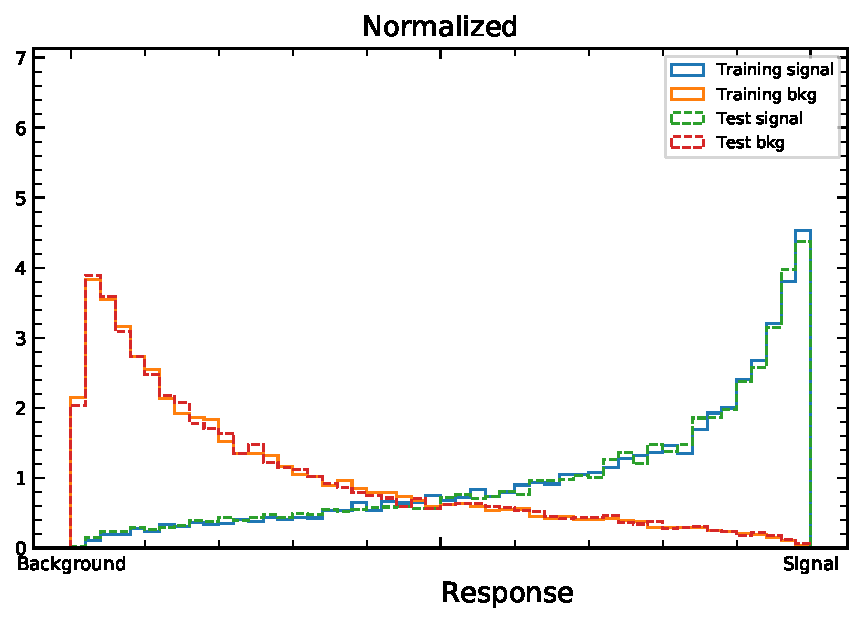
\includegraphics[width=0.95\linewidth]{ubonn-thesis/Chapters/Chapters_06/Figure/CR_4j2b/NormalizedResponse_PLV_4j2b_L27_20_10_06Oct2021.pdf} 
    \caption{} 
    \label{CR:4j2b:NNout} 
  \end{subfigure}%% 
  \vspace*{0.4cm}
  \begin{subfigure}[b]{0.5\linewidth}
    \centering
    \vspace*{-0.2cm}
    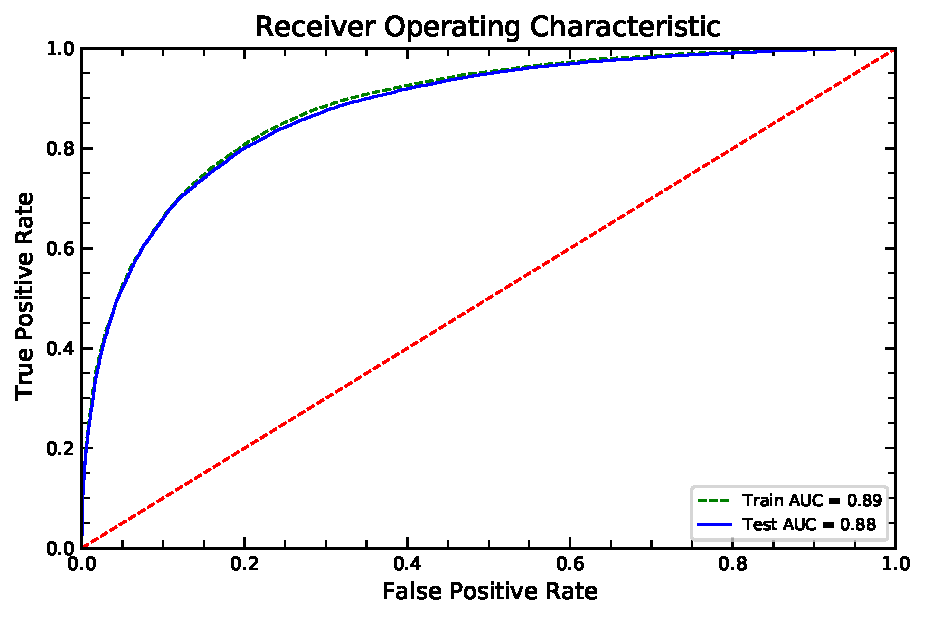
\includegraphics[width=\linewidth]{ubonn-thesis/Chapters/Chapters_06/Figure/CR_4j2b/ROC_PLV_4j2b_L27_20_10_06Oct2021.pdf} 
    % \vspace*{-0.4cm}
    \caption{} 
    \label{CR:4j2b:ROC} 
  \end{subfigure} 
  \vspace*{-0.4cm}
  \begin{subfigure}[b]{0.5\linewidth}
    \centering
    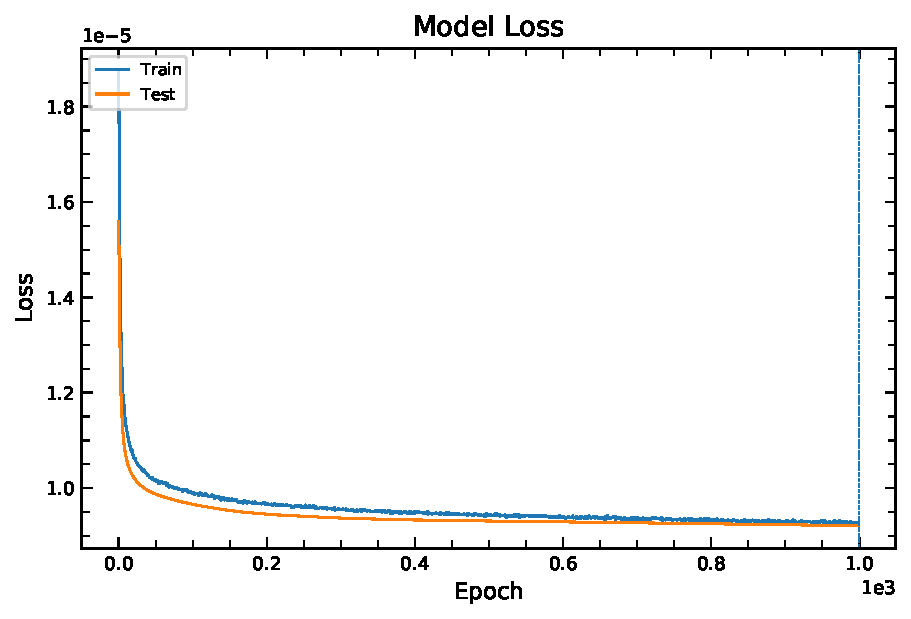
\includegraphics[width=\linewidth]{ubonn-thesis/Chapters/Chapters_06/Figure/CR_4j2b/loss_PLV_4j2b_L27_20_10_06Oct2021.pdf} %\vspace*{-0.4cm}
    \caption{} 
    \label{CR:4j2b:loss} 
  \end{subfigure}%%
  \begin{subfigure}[b]{0.5\linewidth}
    \centering
    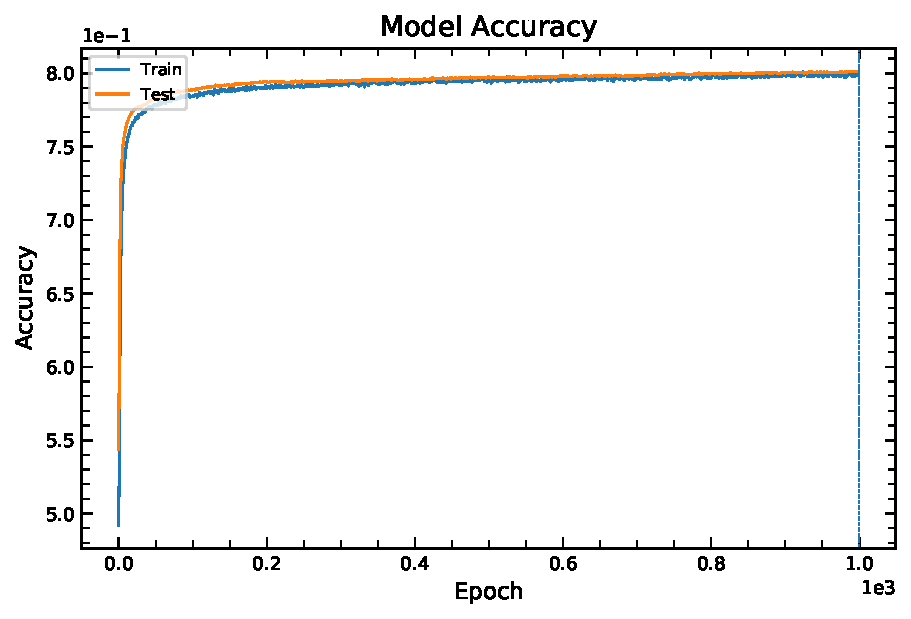
\includegraphics[width=\linewidth]{ubonn-thesis/Chapters/Chapters_06/Figure/CR_4j2b/acc_PLV_4j2b_L27_20_10_06Oct2021.pdf} 
    % \vspace*{-0.4cm}
    \caption{} 
    \label{CR:4j2b:acc} 
  \end{subfigure} 
  \vspace*{-0.3cm}
  \caption{Neural Network training output in the CR 4j2b. (a) shows the normalized response of the NN, (b) shows the ROC curve , (c) shows the loss variation during the training and (d) shows the model accuracy for both training and test samples}
  \label{CR:4j2b:NN} 
\end{figure}



\begin{figure}[ht] 
  \begin{subfigure}[b]{0.5\linewidth}
    \centering
    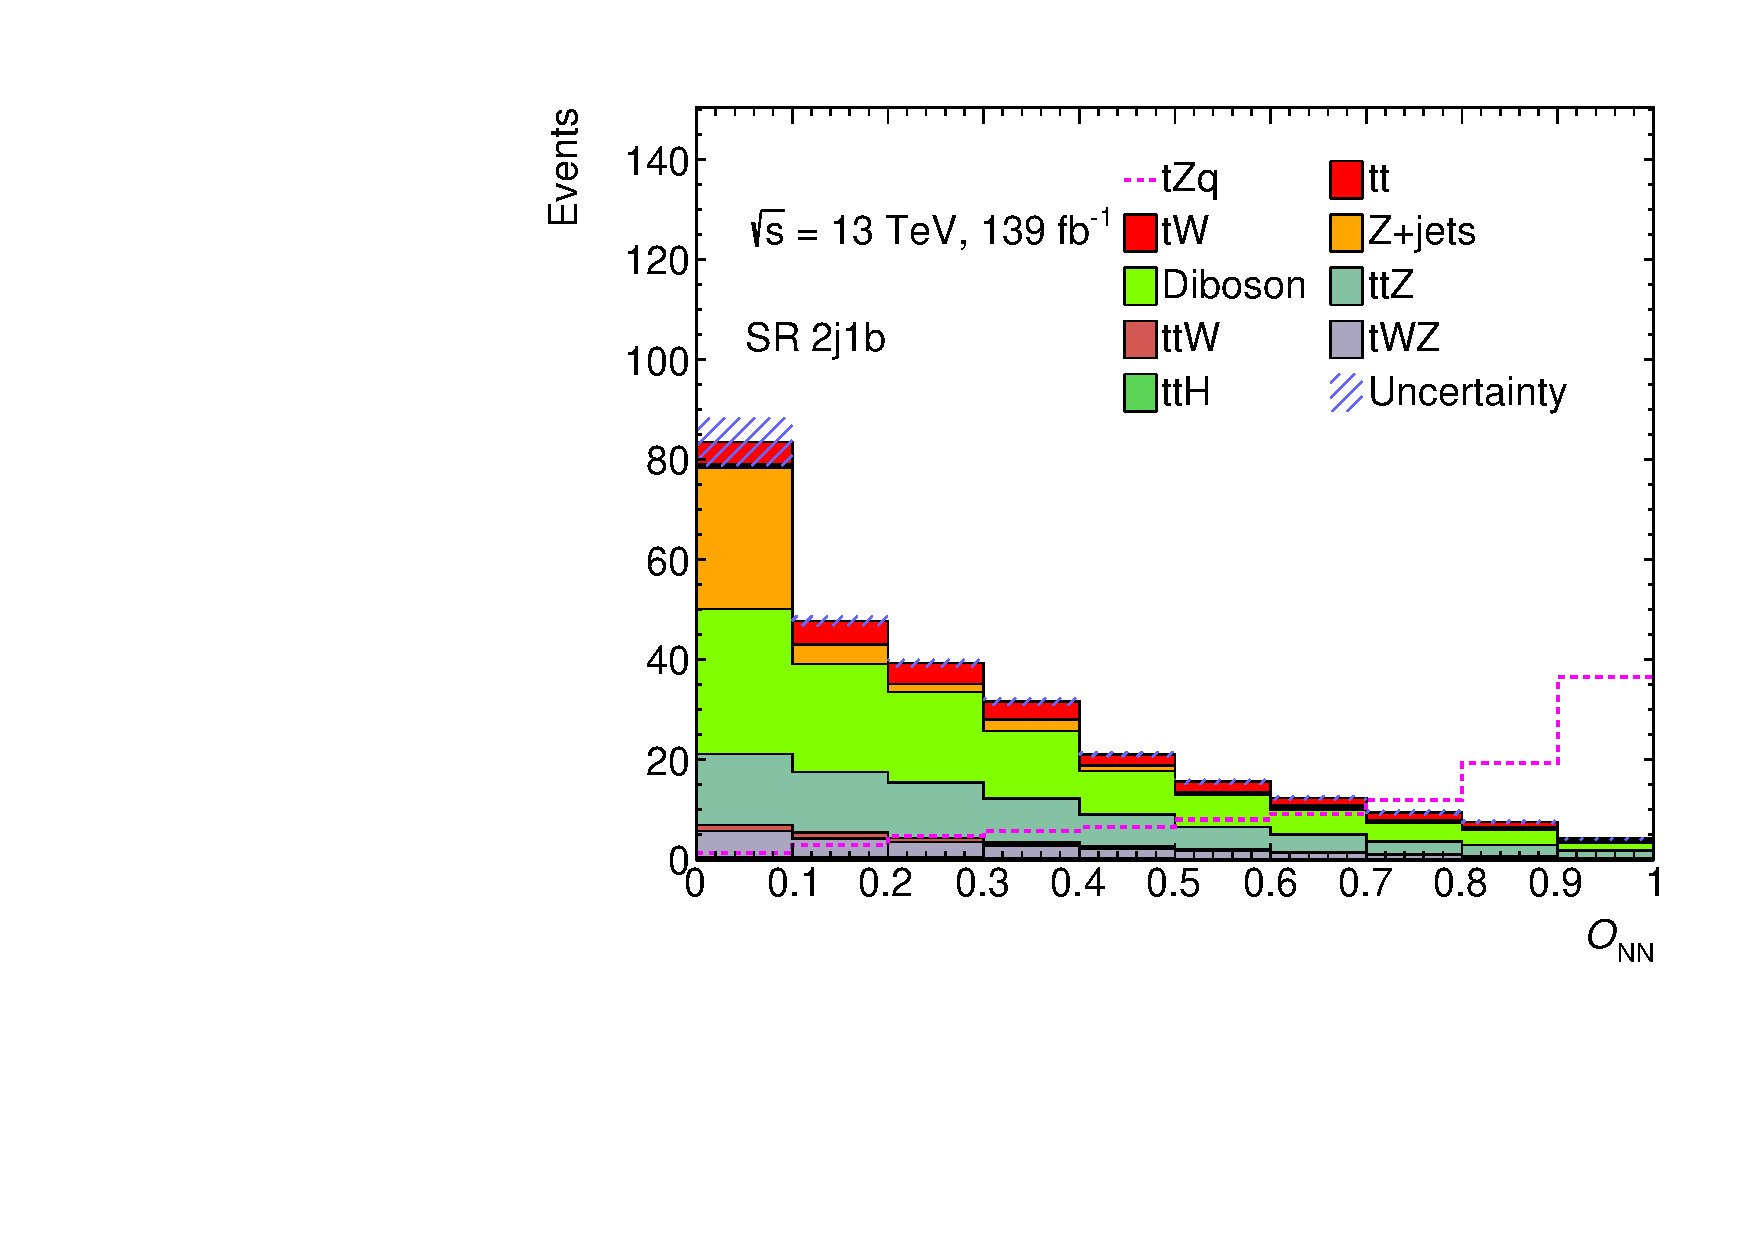
\includegraphics[width=\linewidth]{ubonn-thesis/Chapters/Chapters_06/Figure/Neural Network/SR_2j1b.pdf} 
    \vspace*{-0.9cm}
    \caption{} 
    \label{predict:SR2j1b} 
  \end{subfigure}%% 
  \begin{subfigure}[b]{0.5\linewidth}
    \centering
    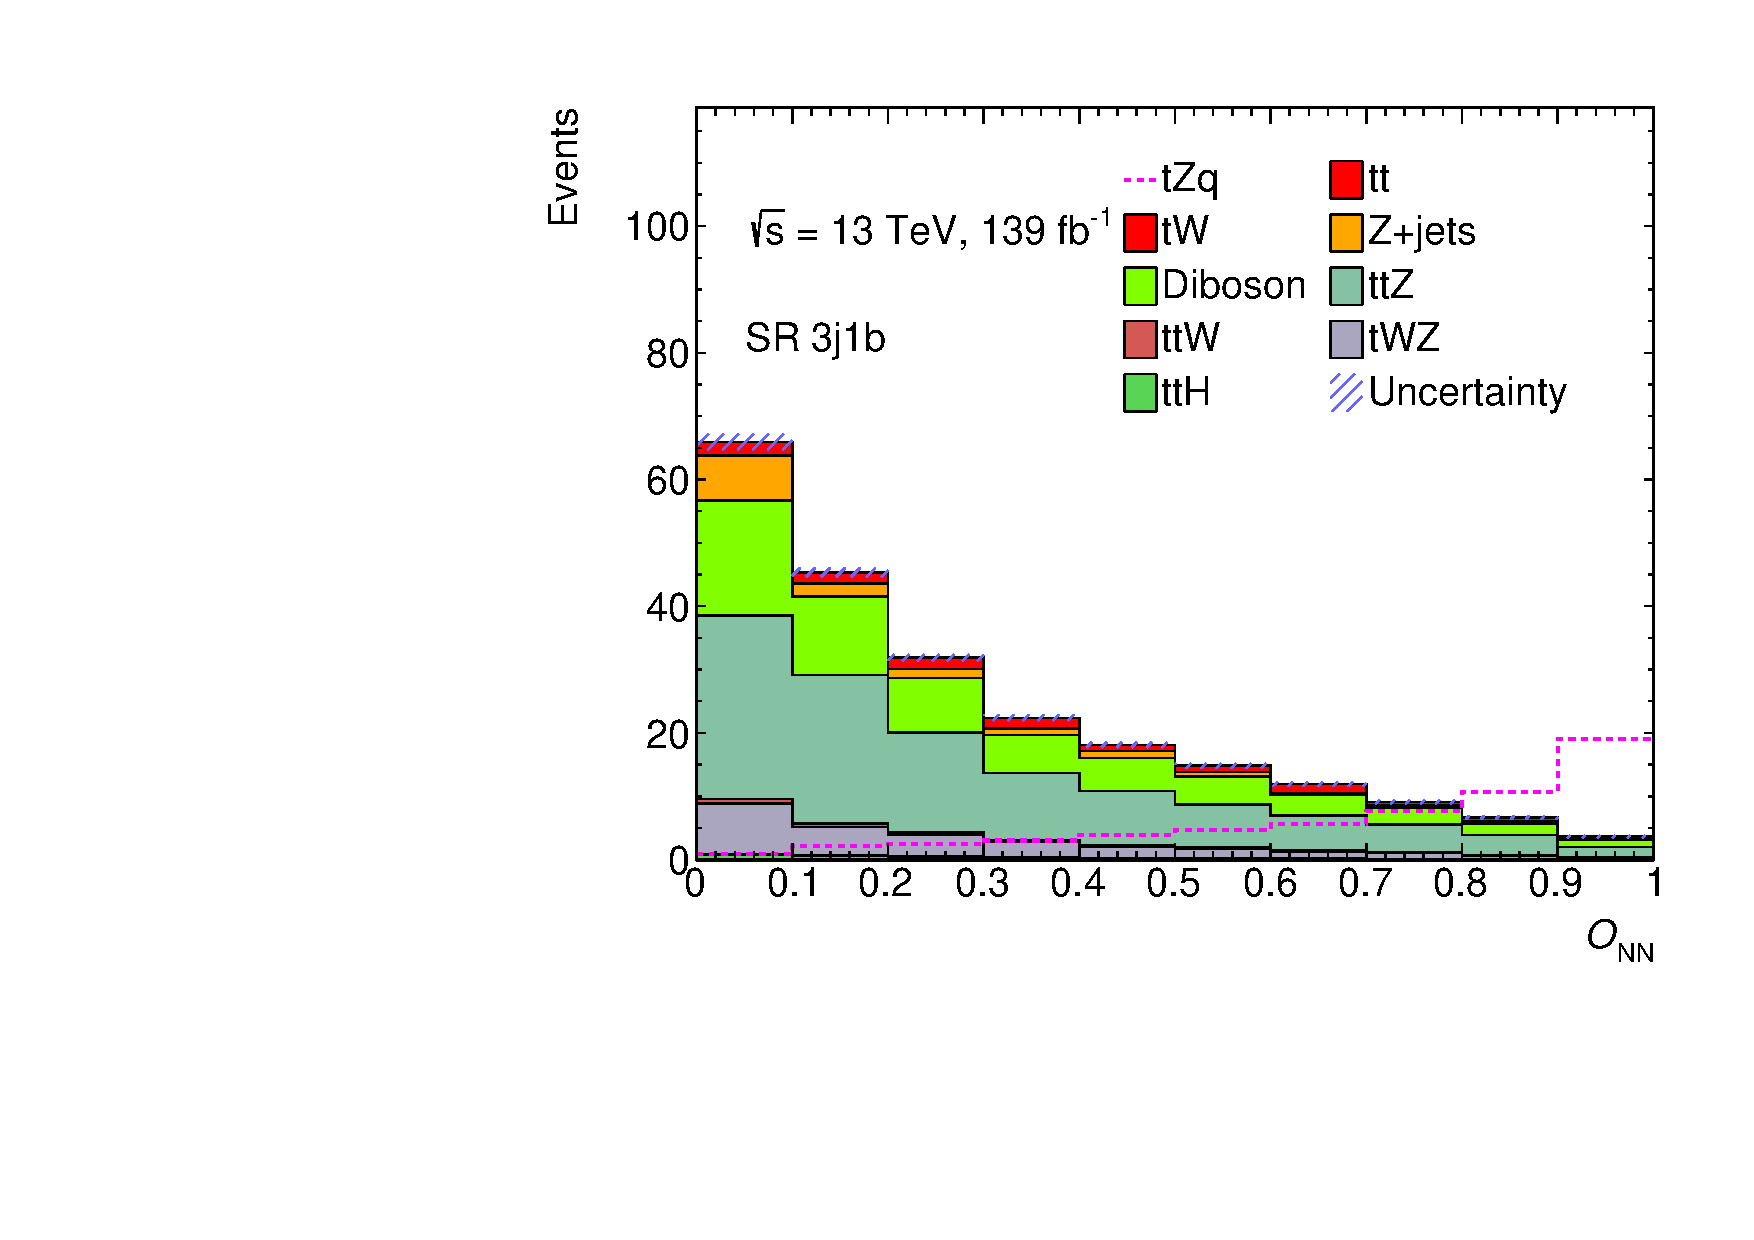
\includegraphics[width=\linewidth]{ubonn-thesis/Chapters/Chapters_06/Figure/Neural Network/SR_3j1b.pdf} 
     \vspace*{-0.9cm}
    \caption{} 
    \label{predict:SR3j1b} 
  \end{subfigure} 
  \begin{subfigure}[b]{0.5\linewidth}
    \centering
    \includegraphics[width=\linewidth]{ubonn-thesis/Chapters/Chapters_06/Figure/Neural Network/CR_3j2b.pdf} 
     \vspace*{-0.9cm}
    \caption{} 
    \label{predict:CR3j2b} 
  \end{subfigure}%%
  \begin{subfigure}[b]{0.5\linewidth}
    \centering
    \includegraphics[width=\linewidth]{ubonn-thesis/Chapters/Chapters_06/Figure/Neural Network/CR_4j2b.pdf} 
    \vspace*{-0.9cm}
    \caption{} 
    \label{predict:CR4j2b} 
  \end{subfigure} 
  \caption{Prediction of the Neural Network training in the SR 2j1b, SR 3j1b, CR 3j2b and CR 4j2b. The outputs are normalized w.r.t. their respective cross-section. The signal tZq is overlayed and the backgrounds are stacked. (a) SR 2j1b, (b) SR 3j1b, (c) CR 3j2b, and (d) CR 4j2b}
  \label{prediction:NN} 
\end{figure}


 The training results for SR 2j1b, CR 3j2b and CR 4j2b are shown in figures \ref{SR:2j1b:NN},  \ref{CR:3j2b:NN}, and \ref{CR:4j2b:NN} respectively whereas training results for SR 3j1b are shown in figures \ref{SR:3j1b:NN(a)} and \ref{SR:3j1b:NN(b)}. In supervised learning, a machine learning algorithm builds a model by examining many examples and attempting to find a model that minimizes the loss. Loss is a number indicating how bad was a single example. If the model's prediction is perfect, the loss is zero; otherwise, the loss is greater. figures \ref{SR:2j1b:loss},  \ref{SR:3j1b:loss},  \ref{CR:3j2b:loss} and  \ref{CR:4j2b:loss}  shows the loss during training at each epoch.

The model accuracy is shown in figures \ref{SR:2j1b:acc}, \ref{SR:3j1b:acc}, \ref{CR:3j2b:acc}, and  \ref{CR:4j2b:acc} which is a way of accessing the performance of a model. It is defined as the number of classifications of a model correctly predicts divided by the total number of predictions made. The normalized neural network response are shown in  figures \ref{SR:2j1b:NNout}, \ref{SR:3j1b:NNout}, \ref{CR:3j2b:NNout}, and \ref{CR:4j2b:NNout} .The output of the signal events accumulate around 1, while the background events accumulate the output around 0. The quality of the training is checked by plotting the receiver operating characteristics (ROC) curves which are shown in figures  \ref{SR:2j1b:ROC}, \ref{SR:3j1b:ROC},  \ref{CR:3j2b:ROC} and  \ref{CR:4j2b:ROC} for SR 2j1b, SR 3j1b, CR 3j2b and CR 4j2b respectively. The area under the ROC curve (AUC) which provides an aggregate measure of performance across can be interpreted as the probability that the model ranks a signal event more highly than a background event. 


\section{Signal extraction - Binned likelihood fit}
\label{sec: Profile_likehihood}
The likelihood function describes the probability of observed data as a function of the parameters of the chosen statistical model. In maximum likelihood estimation, the likelihood function is maximized to obtain specific parameters that are most likely to have generated the observed data. In many cases, the likelihood is a function of more than one parameter but interest focuses on estimation of only one, or at most a few of them while others are considered as nuisance parameters. Profile likelihood is an approach where a likelihood can be written as a function of the only parameter (parameters) of interest. Since in this analysis the selected events are organized in bins, the POI is extracted by performing a binned profile likelihood fit \cite{likelihood2011}. The likelihood is the product of Poisson probability terms for all the bins which can be expressed as:

\begin{equation}
\label{eqn:maxmumlikelihood}
    \mathcal{L} (n \mid \mu, \Vec{\theta} ) = \prod_{i\epsilon bins} \mathcal{P}\left( n_{i} \mid \mu . S_{i}(\theta)+B_{i}(\theta)\right) \times \prod_{j\epsilon syst}\mathcal{G} ( \theta^{0}_{j} \mid \theta_{j}, \Delta \theta_{j} )
\end{equation}

Here, POI is the signal strength $\mu$ which is the ratio between the measured tZq cross-section and the SM prediction $\sigma_{tllq}$ = 102 fb, $n_{i}$ is the observed number of events in bin i, while $S_{i}$ and $B_{i}$ are the predicted numbers of signal and background events; $\Vec{\theta}$ is the set of nuisance parameters introduced for characterizing the impact of systematic uncertainties into the likelihood function  where $\theta = 0$ corresponds to the nominal MC prediction and $\theta = \pm 1$ corresponds to the respective $\pm 1\sigma$ variation and all the nuisance parameters (NPs) are constrained by a Gaussian prior term with $\theta_{j}^{0} = 0$ and $\Delta \theta_{j}^{0} = 1$.


To perform the fit, the TRExFitter software package \cite{trexfitter} is used which combines the functionalities of RooFit \cite{verkerke2003roofit} and RooStats \cite{moneta2011roostats}. It allows to define signal and also control regions which can be fitted simultaneously. Furthermore, it provides many features, for example smoothing of histograms, pruning, and symmetrisation of systematic uncertainties



\section{Systematics uncertainties}
\label{sec:systematics}

Systematic uncertainties are the possible unknown variations in measurements that are not directly caused by data statistics. Many sources of systematic uncertainties are considered in the extraction of the tZq total cross-section. Each source of systematic uncertainty affects the predicted signal and background modeling. The impact of each uncertainty is propagated to each histogram bins yield and is constrained by individual Gaussian nuisance parameters (NPs) in the maximum likelihood fit as shown in eqn. \ref{eqn:maxmumlikelihood}.

\subsection{Sources of systematics uncertainties}

The systematic uncertainties can arise due to imprecise knowledge of the detector acceptance, calibration and resolutions, choice of input parameters in the MC simulations, imprecise measurement of the luminosity or uncertainties on the method used for background. The sources of systematic uncertainties that are used in the fit are introduced below. 

\subsection{Experimental uncertainties}

\subsubsection{Luminosity}
The uncertainty in the combined 2015–2018 integrated luminosity is 1.7 \%. The values is derived with methods described in Ref. \cite{ATLAS-CONF-2019-021} and by using the LUCID-2 detector for the luminosity measurements \cite{Avoni:2018iuv}.

\subsubsection{Pile-up reweighting}

As described in section \ref{subsec:reweightingofMC}, all MC samples are reweighted in order to match the level of pile-up observed in data \cite{Marshall:2014mza}. Uncertainties related to the pile-up scale factors have to be propagated into the fit. An up and a down variations are provided.

\subsubsection{Lepton reconstruction, identification, isolation and trigger}

Reconstruction, identification, isolation and trigger performance for electrons and muons differ between data and MC. To correct these differences, scale factors related to the mentioned procedures are applied. This is done by selecting events that have a clear leptonic signature, such as $Z \rightarrow \mu^{+}\mu^{-}$ and $Z\rightarrow e^{+}e^{-}$ events. The uncertainties are evaluated by varying the lepton and signal selection and from the uncertainties in the background evaluations \cite{lep_syst12012,lep_syst2017}

\subsubsection{Jet vertex tagger efficiency}

For the cross-section measurement, it is necessary to distinguish between pile-up and jets from the hard scattering process. Therefore, the efficiency of the jet vertex tagger (JVT) needs to be precisely known. An uncertainty associated to the JVT scaling factor is assigned, which is estimated by taking into account differences observed when using different MC generators in Z+jets events, statistical uncertainty and additional uncertainty due to residual pile-up contamination \cite{ATLAS:2015ull}.

\subsubsection{Flavour tagging}

A flavour-dependant efficiencies and their uncertainties are evaluated from the data \cite{ATLAS:2015dex}. Efficiencies of heavy flavour jets (b and c jets) need to be corrected by $p_{T}$ dependant scale factors in simulations. The
 uncertainty on the scale factors are de-correlated result in nine eigen-vectors (EV) for b-tag efficiencies,
four EV of c-tag efficiencies and six EV for light-flavour efficiencies.

\subsection{Theoretical uncertainties}

\subsubsection{MC background normalisation}
Normalization uncertainties are assigned to all MC background distributions in order to take into account the theoretical uncertainties on the predicted cross-sections as well as the uncertainties on the acceptances. For the single top-quark backgrounds, acceptance effects are already taken into account in the modelling uncertainties. Therefore, the total uncertainties (PDF + $\alpha_{s}$, and QCD scale uncertainties) on the predicted cross-section is used. The expected overall rate uncertainty for the background processes are shown in table \ref{tab:mcbackroundnormalixation} from ref.\cite{tZq2018} but the fit strategy is applied as discussed in section \ref{sec:strategy}. 

\begin{table}[h!]
     \centering
      \begin{tabular}{@{} *4l  @{}}
      \toprule
       Process & Uncertainty \\
     \midrule
      $t\Bar{t} + tW $ & 7\% \\[0.2ex]
      Z+jets &  15\%\\[0.2ex]
      Diboson  &  30\% \\[0.2ex]
      $t\Bar{t}Z + tWZ$ & 12\% \\[0.2ex]
     $t\Bar{t}H + t\Bar{t}W $ &  15\% \\[0.2ex]
      \bottomrule
 \end{tabular}
 \caption{Overview of normalisation uncertainties for the background processes.}
 \label{tab:mcbackroundnormalixation}
 \end{table}
 
 \subsubsection{Signal PDF and radiation}
 
 The systematic effects due to uncertainties in the parton distribution function, in the renormalization and factorization scales, and in the amount of additional radiation is signal modeling uncertainties. The uncertainty in the renormalization, factorization scales, and in the amount of additional radiation are referred to as "tZq QCD radiation". The tZq PDF uncertainty is 2.2\%, and the tZq QCD radiation is 10.8\% (ref. \cite{tZq2018}). The details on tZq signal modelling uncertainty are given in ref. \cite{tZq2018}.

\subsection{Symmetrizing, smoothing and pruning}

To reduce the complexity and increase the speed and stability of the fit, pruning, symmetrizing and  smoothing procedure is applied within TRExFitter framework. Systematic uncertainties which have an effect smaller than 0.05\% on the normalization are only considered for the shape effect. Uncertainties with an effect smaller than 0.1\% on the shape are only considered
for the normalization effect. MC statistical uncertainties are also removed from the fit if the uncertainty in the specific bin is lower than 0.1\%. 

\label{sec:asimov}


\section{Fitted regions}
\label{subsec:fittedregions}

The SRs included in the fit are designed to maximize sensitivity to the POI, and the CRs are designed to maximally constrain nuisance parameters so as to have maximum information extraction of the POI. The regions and the corresponding distributions that are fitted are summarized in table \ref{tab:fittedregions}. For the SRs and $t\Bar{t}Z$ CRs, the output of NN, $O_{NN}$ distribution is used in the fit. For the diboson CRs, the transverse mass of W boson, $m_{T}(W)$ distribution is used.  The $m_{T}(W)$ distribution also contains Z+jets in the first bin. For the $t\Bar{t}$ CRs a single bin $m_{bj_{f}}$ distribution. Due to relatively low statistics, the used variable is irrelevant.

\begin{table}[h!]
     \centering
      \begin{tabular}{@{} *4l  @{}}
      \toprule
       Region & Distribution & Additional info \\
     \midrule
      SR 2j1b & $O_{NN}$ & {--}\\[0.2ex]
      SR 3j1b & $O_{NN}$ & {--}\\[0.2ex]
      CR diboson 2j0b & $m_{T}(\ell,E_{T}^{miss})$ & {--}\\[0.2ex]
      CR diboson 3j0b & $m_{T}(\ell,E_{T}^{miss})$ & {--}\\[0.2ex]
      CR $t\Bar{t}$ 2j1b & $m_{bj_{f}}$ & Single bin \\[0.2ex]
      CR $t\Bar{t}$ 3j1b & $m_{bj_{f}}$ & Single bin \\[0.2ex]
      CR $t\Bar{t}Z$ 3j2b & $O_{NN}$ & {--}\\[0.2ex]
      CR $t\Bar{t}Z$ 4j2b & $O_{NN}$ & {--}\\[0.2ex]
      \bottomrule
 \end{tabular}
 \caption{Overview of the regions included in the fit}
 \label{tab:fittedregions}
 \end{table}


\subsection{Binning optimization}
\label{subsec:binningoptimization}

To find the best binning for the distributions in each fitted region, the TransfoD method (AutoBin) in TRExFitter is used. The best bins are the one with highest significance. There are two parameters in the AutoBin function ns and nb. When ns = 0 (nb = 0), background (signal) distribution is flat, namely, each bin contains the same number of events. In this optimization, Asimov dataset is used and all systematics are included in the significance calculation (based on TRExFitter) as used in the final fit. The significance for different ns, nb combinations in each fitted regions is given in table \ref{tab:binningoptimization}. The distribution with higher than 10 bins has some empty bins. So, to avoid any empty bins, only 10 bins are used in the SRs. The binning option (7,3) is used as the final binning configuration for SRs. The same process is repeated for the CRs. The binning configuration are: $t\Bar{t}Z$ (2.5,0.5), diboson: (3,0), $t\Bar{t}$: (1,0).

\begin{table}[!h]
\centering
\begin{minipage}{.37\textwidth}
%\centering
\begin{tabular}{@{} *4l @{}}
 \toprule
($n_{b}$,$n_{s}$) & SR 2j1b & SR 3j1b \\[0.2ex] 
 \midrule  
  (12,0) & 10.087 & 6.298 \\[0.2ex]
      (11,1) & 10.207 & 6.404 \\[0.2ex]
      (10,2) & 10.489 & 6.256 \\[0.2ex]
      (9,3) & 10.631 & 6.176 \\[0.2ex]
      (8,4) & 10.6902 & 6.208 \\[0.2ex]
      (7,5) & 10.6904 & 6.068 \\[0.2ex]
      (6,6) & 10.366 & 6.205 \\[0.2ex]
      (5,7) & 10.197 & 6.406 \\[0.2ex]
      (4,8) & 10.160 & 6.050 \\[0.2ex]
 \bottomrule
 \end{tabular}
 \caption*{(a)}
\end{minipage}%
\vspace*{0.4cm}
\centering
\begin{minipage}{.37\textwidth}
%\centering
\begin{tabular}{@{} *4l @{}}
\toprule
($n_{b}$,$n_{s}$) & SR 2j1b & SR 3j1b \\[0.2ex] 
\midrule
     (11,0) & 9.922 & 6.411 \\[0.2ex] 
      (10,1) & 10.246 & 6.263 \\[0.2ex] 
      (9,2) & 10.570 & 6.117 \\[0.2ex] 
      (8,3) & 10.641 & 6.233 \\[0.2ex] 
      (7,4) & 10.687 & 6.070 \\[0.2ex] 
      (6,5) & 10.374 & 6.232 \\[0.2ex] 
      (5,6) & 10.191 &  6.285 \\[0.2ex] 
      (4,7) & 10.039 &  6.038 \\[0.2ex] 
\bottomrule
\end{tabular} 
\caption*{(b)}
\end{minipage} 
\newline
\centering
\begin{minipage}{.37\textwidth}
%\centering
\begin{tabular}{@{} *4l @{}}
 \toprule
 ($n_{b}$,$n_{s}$) & SR 2j1b & SR 3j1b \\[0.2ex] 
\midrule
      (10,0) & 9.938 & 6.267 \\[0.2ex] 
      (9,1) & 10.321 & 6.108 \\[0.2ex] 
      (8,2) & 10.525 & 6.132 \\[0.2ex] 
      (7,3) & 10.602 & 6.065 \\[0.2ex] 
      (6,4) & 10.283 & 6.270 \\[0.2ex] 
      (5,5) & 10.008 & 6.249 \\[0.2ex] 
      (4,6) & 9.985 & 6.043 \\[0.2ex] 
      (3,7) & 9.566 & 5.619 \\[0.2ex] 
\bottomrule
\end{tabular}
\caption*{(c)}
\end{minipage} 
\begin{minipage}{.37\textwidth}
%\centering
\begin{tabular}{@{} *4l @{}}
 \toprule
 ($n_{b}$,$n_{s}$) & SR 2j1b & SR 3j1b \\[0.2ex] 
\midrule
      (8,0) & 9.852 & 6.049 \\[0.2ex]
      (7,1) & 10.215 & 6.052 \\[0.2ex]
      (6,2) & 10.072 & 6.238 \\[0.2ex]
      (5,3) & 9.861 & 6.274 \\[0.2ex]
      (4,4) & 9.938 & 6.054 \\[0.2ex]
      (3,5) & 9.479  & 5.715 \\[0.2ex]
      (2,6) & 9.205 &  5.412 \\[0.2ex]
\bottomrule
\end{tabular} 
\caption*{(d)}
\end{minipage} 
\caption{Median significance with binning for different configuration of $n_{b}$ and $n_{s}$. It is calculated within the TRExFitter framework. (a) Median significance calculated with total number of nbins = 12, (b)  Median significance calculated with total number of nbins = 11, (c)  Median significance calculated with total number of nbins = 10, and (d)  Median significance calculated with total number of nbins = 8}
\label{tab:binningoptimization}
\end{table}

